\section*{Appendix}
This appendix is segmented into the following key parts.

\begin{enumerate}

    \item \textbf{Section \ref{app:sec_proof}} continues the analysis of the eigenspectrum of CPCC-optimized representation matrix and generalizes it for an arbitrary label tree. 

    \item \textbf{Section \ref{app:secB}} discusses additional details about our proposed method \texttt{HypStructure}, its implementation and broader impact of our work. In particular, an overview of the method is first provided, and then we describe hyperparameter settings of our method and the main baselines, followed by extra dataset details and explanation of evaluation metrics.
    
    \item \textbf{Section \ref{app:secC}} reports ablation studies, detailed results on OOD detection and provides additional experimental results and visualizations not included in the main paper due to lack of space.

\end{enumerate}

\section{Details of Eigenspectrum Analysis}
\label{app:sec_proof}
In this section, we first introduce some notations, discuss the setup for our analysis, followed by preliminary lemmas, and then characterize the eigenspectrum of CPCC-based structured representations in \Cref{thm:eigen-generic} for an arbitrary label tree and \Cref{thm:eigen} for a balanced tree presented in the main body.

\paragraph{Proof Sketch} The proof of \Cref{thm:eigen-generic} and \Cref{thm:eigen} relies on the important observation of a \emph{hierarchical} block structure of the covariance matrix of CPCC-regularized features, as shown in \Cref{fig:poincare-matrix}, which will also be supported by \Cref{lem:cos} and \Cref{cor:poi}. \Cref{thm:block} \citep{Cadima_Calheiros_Preto_2010} and \Cref{lem:diag} characterize the eigenvalues of a block correlation matrix induced from a basic tree where the matrix only has three types of values: diagonal values of $1$s, one for within group entry, and another for across group entry. Larger within group entries lead to the larger eigenvalues. \Cref{thm:block} \citep{Cadima_Calheiros_Preto_2010} and \Cref{lem:diag} are then used as the base case for the induction proof of \Cref{thm:eigen}. For an arbitrary tree, in \Cref{thm:eigen-generic}, we use Weyl's Theorem \citep{Weyl_1912} to bound the gap between within group entries and across group entries that leads to the phase transition of eigenvalues.

\paragraph{Setup details} After training with the \texttt{HypStructure} loss till convergence, let us denote the feature matrix as $Z \in \mathbb{R}^{n \times d}$, where each row of $Z$ is a $d$-dimensional vector of an in distribution training sample, and the CPCC is maximized to $1$. We let $C_0 = n, C_1, C_2, \dots, C_H = 1$ be the number of class labels at height $h$ of the tree $\mathcal{T}$. Following the standard pre-processing steps in OOD detection \citep{2021ssd}, we assume that the features are standardized and normalized so that $\mathbb{E}[Z] = \mathbf{0}$ and $\|Z_{i}\|_2 = 1, \forall i$. Besides, we assume that in $\mathcal{T}$, the distance from root node to each leaf node is the same. Otherwise, following \citet{santurkar2021breeds}, we can insert dummy parents or children into the tree to make sure vertices at the same level have similar visual granularity. We then apply CPCC to each node in the extended tree, where each leaf node is one sample. We note that although this is slightly different from the implementation where the leaf nodes are fine class nodes, the distance for samples within fine classes are automatically minimized by classification loss like cross-entropy and supervised contrastive loss. 

Given these assumptions, we want to analyze the eigenspectrum of the inverse sample covariance matrix $\frac{1}{n-1}Z^\top Z$, which is the same as investigating the eigenvalues of $K = ZZ^\top$ where $Z$ is ordered by classes at all levels, i.e., samples having the same fine-grained labels and coarse labels should be placed together. This is because the matrix scaling and permutation will not change the order of singular values. 

Since CPCC (\cref{eq:CPCC}) is a correlation coefficient, when it is maximized, the $n$ by $n$ pairwise Poincaré distance matrix is perfectly correlated with the ground truth pairwise \emph{tree-metric} matrix, where each entry is the tree distance between two samples on the tree, no matter we apply CPCC to leaves or all vertices. This implies that in the similarity matrix $K$, the relative order of entries are the opposite of tree matrix, and it is trivial to show it as follows

\begin{lemma}
    The relative order of entries in $K$ will be the reverse of the order in tree distance.
    \label{lem:cos}
\end{lemma}

\begin{proof}
    When $\norm{u} = \norm{v} = 1$, $\ell_2(u,v)^2 = \norm{u-v}_2^2 = \norm{u}^2 + \norm{v}^2 - 2\langle u,v\rangle = 2 - 2\langle u,v\rangle$. Now considering the CPCC computation, if the CPCC is maximized, the pairwise Euclidean matrix is of the scalar factor of the tree distance matrix. Since each entry of $K$ is the dot product of two samples, the relative order in $K$ is the opposite. 
\end{proof}

\begin{corollary}
    If we use the Poincaré distance (\cref{eq:poincaredistance} in CPCC and let the curvature constant $c = 1$, the statement of cosine distance in Lemma \ref{lem:cos} still holds.
    \label{cor:poi}
\end{corollary}
\begin{proof}
Since the Poincaré distance (\cref{eq:poincaredistance}) is only defined for vectors with magnitude less than $1$, let us consider the case where before the clipping operation, both $u$ and 
$v$ are outside the unit ball. After applying $\text{clip}^1$, $\norm{u} = \norm{v} = 1 - \epsilon$, where $\epsilon$ is a small constant ($10^{-5}$). Then $\norm{u}^2 = (1 - \epsilon)^2 = 1 - 2\epsilon + \epsilon^2$. Define $2\epsilon - \epsilon^2$ as $\xi$, making $\norm{u}^2 := 1 - \xi$ where $\xi$ is also a small constant such that $O(\xi^2)$ is negligible.

\begin{align*}
    \textnormal{Poincaré}(u,v) &= 2\ln\frac{\norm{u - v} + \sqrt{\norm{u}^2\norm{v}^2 - 2 u \cdot v + 1}}{\sqrt{(1 - \norm{u}^2)(1 - \norm{v}^2)}} \\
    &= 2\ln \frac{\norm{u - v} + \sqrt{2 - 2u\cdot v - 2\xi + \xi^2}}{\xi} \\
    &\approx 2\ln \frac{\norm{u - v} + \sqrt{2 - 2u\cdot v - 2\xi}}{\xi} \\
    &= 2\ln \frac{\norm{u - v} + \sqrt{\norm{u}^2 + \norm{v}^2 - 2u\cdot v}}{\xi} \\
    &= 2\ln \frac{2\norm{u - v}}{\xi}
\end{align*}
We can see that the Poincaré distance monotonically increases with Euclidean distances $\norm{u-v}$. This property ensures the relative order of any two entries for Euclidean CPCC and Poincare CPCC matrices in $K$ to be the same. Then, we can argue about the structure of $K$, either Euclidean or Poincare, to have the hierarchical diagonalized structure as in \Cref{fig:poincare-matrix}. So any statement applied for a Poincaré version of CPCC will also hold for the Euclidean CPCC counterpart.
\end{proof}

For each level of the tree, due to the optimization of CPCC loss, the corresponding off diagonal entries of $K$, which represent the intra-level-class similarities, are much smaller than inter-level-class values. We thus have a symmetric similarity matrix that takes on the following structure, where the red regions are greater than orange regions, which are further greater than the blue regions.

\begin{equation*}
    K = \left[\begin{array}{cc:cc:cc:cc:c}
\textcolor{red}{1} & \textcolor{red}{r_{11}^1}  & \textcolor{orange}{r_{12}^2} & \textcolor{orange}{r_{12}^2} & \textcolor{blue}{r_{13}^3} & \textcolor{blue}{r_{13}^3} & \textcolor{blue}{r_{14}^3} & \textcolor{blue}{r_{14}^3} & \dots \\
\textcolor{red}{r_{11}^1} & \textcolor{red}{1}  & \textcolor{orange}{r_{12}^2} & \textcolor{orange}{r_{12}^2} & \textcolor{blue}{r_{13}^3} & \textcolor{blue}{r_{13}^3} & \textcolor{blue}{r_{14}^3} & \textcolor{blue}{r_{14}^3} & \dots \\ \hdashline
r_{12}^2 & r_{12}^2 & \textcolor{red}{1}  & \textcolor{red}{r_{22}^1} & \textcolor{blue}{r_{23}^3} & \textcolor{blue}{r_{23}^3} & \textcolor{blue}{r_{24}^3} & \textcolor{blue}{r_{24}^3} & \dots \\
r_{12}^2 & r_{12}^2 & \textcolor{red}{r_{22}^1}  & \textcolor{red}{1} & \textcolor{blue}{r_{23}^3} & \textcolor{blue}{r_{23}^3} & \textcolor{blue}{r_{24}^3} & \textcolor{blue}{r_{24}^3} & \dots \\ \hdashline
r_{13}^3 & r_{13}^3 & r_{23}^3  & r_{23}^3 & \textcolor{red}{1} & \textcolor{red}{r_{33}^1} & \textcolor{orange}{r_{34}^2} & \textcolor{orange}{r_{34}^2} & \dots \\

r_{13}^3 & r_{13}^3 &  r_{23}^3 & r_{23}^3 & \textcolor{red}{r_{33}^1} & \textcolor{red}{1} & \textcolor{orange}{r_{34}^2}  & \textcolor{orange}{r_{34}^2}  & \dots \\ \hdashline
r_{14}^3 & r_{14}^3 &  r_{24}^3  & r_{24}^3 & r_{34}^2 & r_{34}^2 & \textcolor{red}{1} & \textcolor{red}{r_{44}^1} & \dots \\
r_{14}^3 & r_{14}^3 &  r_{24}^3 & r_{24}^3 & r_{34}^2 & r_{34}^2 & \textcolor{red}{r_{44}^1}  & \textcolor{red}{1} & \dots \\ \hdashline
\dots & \dots & \dots & \dots & \dots & \dots & \dots & \dots & \dots
\end{array}\right]
\end{equation*}

Each non-diagonal entry is called $r_{ij}^h$ where $i,j$ are the index of the diagonal block, or the \emph{finest} label id of one sample, and $h$ is the height of the lowest common ancestor of the two samples in the row and the column. Since every two leaves sharing the lowest common ancestor of the same height have the same tree distance, each entry of $K$ with the same superscript will be the same so we can drop the $i,j$ subscript in the notation. The size of each block is defined by the number of samples within one label. Then, the shown submatrix of $K$ corresponds to the following tree in \Cref{fig:subtree}. Next, we present several useful lemmas and theorems.

\begin{figure}[ht]
    \centering
    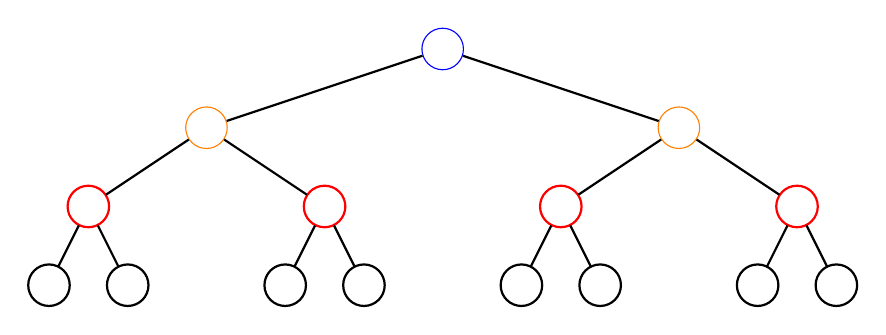
\begin{tikzpicture}[
    every node/.style={circle, draw, inner sep=2pt, minimum size=1.5em},
    level 1/.style={sibling distance=60mm, level distance=10mm},
    level 2/.style={sibling distance=30mm, level distance=10mm},
    level 3/.style={sibling distance=10mm, level distance=10mm},
    level 4/.style={sibling distance=5mm, level distance=10mm},
    edge from parent/.style={draw, black, thick}
]
\node [draw=blue] {} 
    child {node [draw=orange] {} 
        child {node [draw=red] {} 
            child {node [draw=black] {}} 
            child {node [draw=black] {}} 
        }
        child {node [draw=red] {} 
            child {node [draw=black] {}} 
            child {node [draw=black] {}} 
        }
    }
    child {node [draw=orange] {} 
        child {node [draw=red] {} 
            child {node [draw=black] {}} 
            child {node [draw=black] {}} 
        }
        child {node [draw=red] {} 
            child {node [draw=black] {}} 
            child {node [draw=black] {}} 
        }
    };
\end{tikzpicture}
\caption{Subtree corresponds to the shown submatrix of $K$.}
\label{fig:subtree}
\end{figure}


\begin{theorem}[\citep{Cadima_Calheiros_Preto_2010}]
\label{thm:block}
    Let $R$ be a $p \times p$ full-rank correlation matrix that has a $k$-group block structure, with groups of size $p_i$ ($i = 1 : k$, $\sum\limits_{i=1}^k p_i = p$). Let $r_{ii}$ be the correlation for any pair of different variables within group $i$. Let $r_{ij}$ be the common correlation between any variable in group $i$ and $j$. Denote the mean of the $i$-th diagonal block of $R$ by $\overline{R_i} = (1/p_i)(1 + (p_i - 1)r_{ii})$. Then:
    \begin{enumerate}
        \item $R$ has $p_i - 1$ eigenvalues $1 - r_{ii}$ $(i = 1 : k)$.
        \item The rest of the eigenvalues are those from $k \times k$ symmetric matrix $A$ whose diagonal elements are $a_{ii} = p_i\overline{R_i}$ and whose off-diagonal elements are $a_{ij} = \sqrt{p_i\cdot p_j}r_{ij}$.
    \end{enumerate}
\end{theorem}

\begin{lemma}
\label{lem:diag}
    Given $d$ by $d$ matrix $M$ where $M_{ii} = 1,$ $\forall i \in [d],$ and $M_{ij} = p$ otherwise, i.e., 
    \begin{equation*}
        M = \begin{bmatrix} 
            1 & p & \dots & \dots & p \\
            p & \ddots &  &  & \vdots\\
            \vdots & & 1  &  & \vdots\\
            \vdots & &   & \ddots & p\\
            p &   \dots     & \dots  & p & 1
            \end{bmatrix}
    \end{equation*}
    it has eigenvalues $\lambda_1 = 1 + p(d-1)$ and $\lambda_2 = \dots = \lambda_d = 1 - p$.
\end{lemma}
\begin{proof}
    Using the definition of eigenvalues, we want to compute the determinant of matrix 
    \begin{equation*}
        \begin{bmatrix} 
            1 - \lambda & p & \dots & \dots & p \\
            p & \ddots &  &  & \vdots\\
            \vdots & & 1 - \lambda  &  & \vdots\\
            \vdots & &   & \ddots & p\\
            p &   \dots     & \dots  & p & 1 - \lambda
            \end{bmatrix}
    \end{equation*}
    Adding the second till the last row to the first row, we have
    \begin{equation*}
    \begin{bmatrix} 
            1 - \lambda + (d-1)p & 1 - \lambda + (d-1)p & \dots & \dots & 1 - \lambda + (d-1)p \\
            p & \ddots &  &  & \vdots\\
            \vdots & & 1 - \lambda  &  & \vdots\\
            \vdots & &   & \ddots & p\\
            p &   \dots     & \dots  & p & 1 - \lambda
    \end{bmatrix}
    \end{equation*}
    Dividing the first row by $1 - \lambda + (d-1)p$, we now have 
    \begin{equation*}
    \begin{bmatrix} 
            1 & 1 & \dots & \dots & 1 \\
            p & \ddots &  &  & \vdots\\
            \vdots & & 1 - \lambda  &  & \vdots\\
            \vdots & &   & \ddots & p\\
            p &   \dots     & \dots  & p & 1 - \lambda
    \end{bmatrix}
    \end{equation*}
    Subtracting the second till the last row by $p$ times the first row results in an upper triangular matrix
    \begin{equation*}
    \begin{bmatrix} 
            1 & 1 & \dots & \dots & 1 \\
            0 & 1 - \lambda - p &  &  & 0\\
            \vdots & & 1 - \lambda - p  &  & \vdots\\
            \vdots & &   & \ddots & 0\\
            0 &   \dots     & \dots  & 0 & 1 - \lambda - p
    \end{bmatrix}
    \end{equation*}
    Thus, $\det(M - \lambda I) = (1 - \lambda + (d-1)p)(1 - \lambda - p)^{d-1}$.
\end{proof}

Notice that Lemma \ref{lem:diag} is a special case of Theorem \ref{thm:block} where the label tree is a two level basic tree with the root node and $d$ leaves in the second label all being the direct children of the root node. Now we can leverage Theorem \ref{thm:block} and Lemma \ref{lem:diag} to investigate the eigenspectrum of $K$ by proving the following theorem:

\begin{restatable}[\textbf{Eigenspectrum of CPCC-based Structured Representation}]{theorem}{imbalanced}
    \label{thm:eigen-generic} 
    If $\mathcal{T}$ is a tree whose root node has height $H$ where each level has $C_h$ nodes, $h \in [0,H]$. $K = ZZ^\top$ is a block structured correlation matrix as a result of CPCC optimization, where each off-diagonal entry $\in [-1,1]$ can be written as $r^h$ and $h$ is the height of the lowest common ancestor of the $i$-th row and the 00$j$-th column sample. Let $\Delta = r^1 - r^h$, $p_i, i \in [C_h]$ be the number of children for nodes at height $h$, and $p_\text{max}$ be the maximum. For any $h \geq 1$, if $r^h \geq M \geq 0$, $r^{h+1} \leq m$, then 
    \begin{enumerate}[(i)]
        \item We have $C_0 - C_h$ eigenvalues, that come from the eigenvalues of a $C_0 \times C_0$ matrix sharing the same $C_h$ of $p_i \times p_i$ diagonal blocks from $K$ subtracting $r^h$, and off diagonal values are all zero.
        \item The rest of $C_h$ eigenvalues come from a $C_h \times C_h$ matrix, whose diagonal entries are the mean of each $p_i \times p_i$ diagonal block from $K$, and the off diagonal entries are $\sqrt{p_ip_j}r_{ij}$ where $r_{ij}$ is the correlation between node $i$ and node $j$ of height $h$.
        \item If $m \leq \frac{M - 2\Delta(p_\text{max} - 1)}{p_\text{max}(C_h-1)}$, $C_0 - C_h$ eigenvalues are all smaller than $C_h$ eigenvalues.
    \end{enumerate}
\end{restatable}

\begin{proof}
    Part (i) and (ii) can be extended from the proof of Theorem \ref{thm:block}. Let $G$ be the $n \times C_h$ matrix where $G_{ij} = 1$ if the $i$-th sample is in group $j$, otherwise $G_{ij} = 0$. For any $n - C_h$ eigenvectors in the orthogonal complement of the column space of $G$, the eigenvector of $K$ is also the eigenvector of 
\begin{equation*}
    \begin{bmatrix}
    K_1 & \mathbf{0} & \cdots & \mathbf{0} \\
    \mathbf{0} & K_2 & \cdots & \mathbf{0} \\
    \vdots & \vdots & \ddots & \vdots \\
    \mathbf{0} & \mathbf{0} & \cdots & K_k
    \end{bmatrix}
\end{equation*}

    where due to the hierarchical structure of block matrix, $K_i$ has the format of 

\begin{equation*}
    \begin{bmatrix}
1 - r^h & r^1 - r^h & \cdots & r^j - r^h & 0 & \cdots & 0 \\
r^1 - r^h & 1 - r^h & \cdots & 0 & 0 & \cdots & 0 \\
\vdots & \vdots & \ddots & \vdots & \vdots & & \vdots \\
r^j - r^h & 0 & \cdots & 1 - r^h & 0 & \cdots & 0 \\
0 & 0 & \cdots & 0 & 1 - r^h & \cdots & 0 \\
\vdots & \vdots & & \vdots & \vdots & \ddots & \vdots \\
0 & 0 & \cdots & 0 & 0 & \cdots & 1 - r^h
\end{bmatrix}
\end{equation*}

    The rest of $C_h$ eigenvectors come from the symmetric $C_h \times C_h$ matrix $A = (G^\top G)^{-1/2}(G^\top KG)(G^\top G)^{-1/2}$, by some basica algebra, we know $a_{ij} = \frac{1}{\sqrt{p_i}} \cdot (\text{sum of all } r_{ij} \text{ entries in } p_i \times p_j \text{ block}) \cdot \frac{1}{\sqrt{p_j}}$. For more details, we refer the reader to Theorem 3.1 in \citet{Cadima_Calheiros_Preto_2010} where $C_1 = k$ using their notation.

    Since the largest absolute value of $K$'s eigenvalues, is bounded above by the largest row sum of the absolute values of $K$ \citep{Horn_Johnson_2012}, first $n - C_h$ eigenvectors are bounded above by $U = \max_{i}(1 - r^h)+(p_i - 1)(r^1 - r^h) = (1 - r^h) + (p_\text{max} - 1)\Delta$.

    On the other hand, for the rest of $C_h$ eigenvalues, we analyze matrix $A$:
    \begin{align*}
        A &\leq A_1 + A_2 \\
          &:=
        \begin{bmatrix}
        1 + (p_1 - 1)r^h & 0 & \cdots & 0 \\
        0 & 1 + (p_2 - 1)r^h & \cdots & 0 \\
        \vdots & \vdots & \ddots & \vdots \\
        0 & 0 & \cdots & 1 + (p_k - 1)r^h
        \end{bmatrix}\\
        &+ \begin{bmatrix}
(p_{\text{max}} - 1)(r^1 - r^h) & p_{\text{max}}m & \cdots & p_{\text{max}}m \\
p_{\text{max}}m & (p_{\text{max}} - 1)(r^1 - r^h) & \cdots & p_{\text{max}}m \\
\vdots & \vdots & \ddots & \vdots \\
p_{\text{max}}m & p_{\text{max}}m & \cdots & (p_{\text{max}} - 1)(r^1 - r^h)
\end{bmatrix}
    \end{align*}

   The inequality comes from the effect of the maximization of CPCC that $r^1 \geq \cdots r^h \geq r^{h+1} \geq \cdots r^H$ and $r^h \leq m$. The eigenvalues of $A_1, A_2$ have the analytical form, where $A_1$'s eigenvalues have the form of $1 + (p_i - 1)r^h$ and $A_2$'s eigenvalues can be derived by Lemma \ref{lem:diag}. By Weyl's inequality \citep{Weyl_1912}, the minimum of these $C_h$ eigenvalues is at least $L = (1 + (p_\text{min} - 1)r^h) - [(p_\text{max} - 1)\Delta - p_\text{max}m + kp_\text{max}m] \geq (1 + (1 - 1)r^h) - [(p_\text{max} - 1)\Delta - p_\text{max}m + kp_\text{max}m]$.

    To guarantee eigenvalues from Part (ii) are larger, we want $L \geq U$. We solve this inequality with $m$, and we will get the desired range of $m$.
\end{proof}

When $r^h = r^1$ in Theorem \ref{thm:eigen-generic}, we have $\Delta = 0$. Therefore, for a three level basic tree with only $r^1, r^2$, if $m \leq M/(p_\text{max}(C_1-1))$, $C_0 - C_1$ eigenvalues are all smaller than $C_1$ eigenvalues. In general, we have shown that when $m$, i.e., the across group similarity is sufficiently small, the eigenvalue gap always exists. When the label tree $\mathcal{T}$ is balanced, we can further specify the expression of each eigenvalue and the amount of eigenvalue gaps.


We now formally restate the Theorem 4.1 from the main paper and give its proof.

\balanced*


\begin{proof}

    From Corollary \ref{cor:poi}, we know that $K \in \mathbb{R}^{C_0 \times C_0}$ has a block-wise structure. 

    Since all statements are presented recursively, we prove the theorem by structural induction on the height of the tree.

    The base case is Lemma \ref{lem:diag} with a two level hierarchy tree where only (i) and (iii) are applicable, and $p = r^1, C_0 = d, C_1 = 1$. By Lemma \ref{lem:diag}, $K$ has $C_0 - 1$ eigenvalues as $\lambda_0 = 1 - r^1$, and one eigenvalue as $\lambda_1 = 1 + (C_0 - 1)r^1 = (1 - r^1) + r^1 / C_0^{-1}$.

    Let us now assume that the theorem is true for the balanced tree whose root node is at height $H-1$. Then if we have a tree with height $H$. We call the resulting matrix $K_H$. 
    
    By the first bullet point of Theorem \ref{thm:block} we directly get $\lambda_0$ from (i). Then by the second bullet point of Theorem \ref{thm:block}, the rest of the eigenvalues are from the symmetric matrix $A_{H-1} \in \mathbb{R}^{C_1 \times C_1}$ whose diagonal elements are $\gamma = 1 + (C_0/C_1 - 1)r^1$ and whose off diagonal elements are $C_0/C_1 \cdot r^j$ for $j \geq 2$. 
    
    The key is to observe that $A_{H-1}$ is still a block structured matrix. After $A_{H-1}$ is scaled by $\gamma$, the resulting matrix can be also seen as a result of maximizing CPCC where the off diagonal blocks have smaller values. 

    Applying the hypothesis induction, we then know the expression of eigenvalues for $A_{H-1}$ as

    \begin{enumerate}[(i)]
        \item we have $C_1 - C_2$ eigenvalues of the form 
        \begin{align*}
            \lambda_1 &= \gamma(1 - \frac{r^2 C_0/C_1 }{\gamma}) \\
            &= \gamma - \frac{C_0}{C_1}r^2 \\
            &= 1 + (\frac{C_0}{C_1} - 1)r^1 - \frac{C_0}{C_1}r^2 \\
            &= 1 - r^1 + \frac{C_0}{C_1}(r^1 - r^2) \\
            &= \lambda_0 +  \frac{C_0}{C_1}(r^1 - r^2)
        \end{align*}
        \item For $0 < h \leq H-2$, we have $C_{h+1} - C_{h+2}$ eigenvalues of the form
        \begin{align*}
            \lambda_{h+1} - \lambda_{h} &= \gamma\frac{C_0}{C_1} \left(\frac{r^{h+1}}{\gamma} - \frac{r^{h+2}}{\gamma}\right)\frac{C_1}{C_{h+1}}\\
            \lambda_{h+1} &= \lambda_h + (r^{h+1} - r^{h+2})\frac{C_0}{C_{h+1}}
        \end{align*}
        \item The last eigenvalue is 
        \begin{align*}
            \lambda_H - \lambda_{H-1} &= C_1r^H/\gamma \cdot \frac{C_0}{C_1} \gamma \\
            &= C_0 r^{H}
        \end{align*}
    \end{enumerate}
    Therefore, we proved the theorem by showing the induction step from $K_{H-1}$ to $K_{H}$ holds. 
\end{proof}


Note that the true symmetric covariance matrix $K'$ might not be  having the exact format as $K$, but it can be seen as a perturbation of $K$ where $\norm{K' - K} \leq \epsilon$, $\epsilon$ is a small constant. By Weyl's inequality \citep{Weyl_1912}, the approximation error of each eigenvalue is bounded by $[\lambda_i - \epsilon, \lambda_i + \epsilon]$. 



\section{Additional Algorithm and Experimental Details}
\label{app:secB} 

In this section, we first provide an overview of our algorithm, followed by a discussion on the choice of the \emph{flat} loss and additional experimental details about the training and evaluation metrics. 


\subsection{Broader Impact Statement}
\label{app:broader_impact} 
Our work proposes \texttt{HypStructure}, a structured hyperbolic regularization approach to embed hierarchical information into the learnt representations. This provides significant advancements in understanding and utilizing hierarchical real-world data, particularly for tasks such as representation learning, classification and OOD detection, and we recognize both positive societal impacts and potential risks of this work. 
The ability to better model hierarchical data in a structured and interpretable fashion is particularly helpful for domains such as AI for science and healthcare, where the learnt representations will be more reflective of the underlying relationships in the domain space. Additionally, the low-dimensional capabilities of hyperbolic geometry can lead to gains in computational efficiency and reduce the carbon footprint in large scale machine learning. However, real-world hierarchical data often incorporates existing biases which may be amplified by structured representation learning, and hence it is important to incorporate fairness constraints to mitigate this risk.


\subsection{Pseudocode for \texttt{HypStructure}}
\label{app:pseudocode} 

\begin{algorithm}[ht]
\caption{\texttt{HypStructure}: \underline{Hyp}erbolic \underline{Structure}d Representation Learning}
\label{alg:hypstructure}
\begin{algorithmic}[1]
\Require Batch size $B$, Label tree $\mathcal{T}= (V, E, e)$, Number of epochs $K$, Task Loss formulation $\ell_\text{Flat}$, Encoder $f_\theta$, Classifier Head $g_{w}$, Learning Rate $\eta$, Hyperparameters $\alpha, \beta$ 

\State Initialize model parameters: 
$\theta$, $w$
\For {epoch = $1, 2, \ldots K$}
    \For {batch = $1, 2, \dots, B$}
    \State Get image-label pairs: $\{(\vx_i, y_i)\}_{i=1}^{B}$
    \State Forward pass to compute the representations: $(\vz_1 \dots \vz_{B}) \gets (f_{\theta}(\vx_1) \dots (f_{\theta}(\vx_{B})) $  
    \State Compute the Task loss: $\ell_{\text{Flat}}(g_{w}(\vz_i), y_i)$
    \State Get hyperbolic representations using exp. map (\cref{eq:hyp_maps}): $\tilde{\vz}_i \gets \exp_\mathbf{0}^c(\vz_i)$
    \State Calculate class prototypes using hyp. Averaging (\cref{eq:hypave}): $\omega_i \gets \text{HypAve}_K(\tilde{\vz}_{1}^v, \dots \tilde{\vz}_{j}^v)$ 
    \State Compute pairwise hyp. distances (\cref{eq:poincaredistance})  $ \forall v_i, v_j \in V:  \rho(v_i, v_j) \gets d_{\mathbb{B}_c}(\omega_i, \omega_j) $
    \State Get hyp. CPCC loss (\cref{eq:CPCC}: $\hypcpcc(\tmetric, \rho)$
    \State Compute hyp. centering loss using (\Cref{eq:hypave}): $\ell_\text{center} = \norm{\text{HypAve}_B(\tilde{\vz}_1, \dots, \tilde{\vz}_{B}})$

    \State Get total loss using \Cref{eq:objective_hyp}: $\mathcal{L}(\mathcal{D}_B)$
    \State Compute Gradients for learnable parameters at time $t$:  $\mathbf{u_t}(\theta,w) \gets \nabla_{\theta, w}\mathcal{L}(\mathcal{D}_B)$ 
    \State Refresh the parameters: $(\theta,w)_{t+1} \gets (\theta,w)_{t} - \frac{\eta}{B} \mathbf{u_t}(\theta,w)$ 

    \EndFor 
\EndFor
\Ensure $(\vz_1, \dots \vz_N);\theta,w$
\end{algorithmic}
\end{algorithm}

The training scheme for our \texttt{HypStructure} based structured regularization framework is provided in \Cref{alg:hypstructure}. At a high level, in \texttt{HypStructure}, we optimize a combination of the following two losses: (1) a \emph{hyperbolic CPCC} loss to encourage the representations in the hyperbolic space to correspond with the label hierarchy, (2) a \emph{hyperbolic centering} loss to position the representation corresponding to the root of the node at the centre of the \Poincare ball and the children nodes around it. 


\subsection{Choice of Flat loss}

We use the Supervised Contrastive \citep{2020supcon} (\texttt{SupCon}) loss as the first choice for a \emph{flat} loss in our experimentation. Let $q_y$ be the one-hot vector with the $y$-th index as 1. The Cross Entropy (\texttt{CE}) loss, defined between the predictions  $g\circ f_\theta(\vx)$ and the labels $y$, as $\lce(g\circ f(\vx), y) := - \sum_{i\in[k]}q_i\log(g(f(\vx))_i)$ has been used quite extensively in large-scale classification problems in the literature \citep{cubuk2019autoaugment, cubuk1909randaugment, kolesnikov2019large, xie2020self}.  However, several shortcoming of the \texttt{CE} loss, such as lack of robustness \citep{sukhbaatar2014training, zhang2018generalized} and poor generalization \citep{ elsayed2018large, liu2016large} have been discovered in recent research. Contrastive learning has emerged as a viable alternative to the \texttt{CE} loss, to address these shortcomings \citep{chen2020simple, wu2018unsupervised, henaff2020data, tian2020contrastive, hjelm2018learning, he2020momentum}. The underlying principle for these methods is to \emph{pull} together embeddings for positive pairs and \emph{push} apart the embeddings for negative samples, in the feature space. In the absence of labels, positive samples are created by data augmentations of images and negative samples are randomly chosen from the minibatch.  However, when the labels are available, the class information can be leveraged to extend this methodology as a Supervised Contrastive loss (\texttt{SupCon}) by \emph{pulling} together embeddings from the same class, and \emph{pushing} apart the embeddings from different classes. This offers a more stable solution for a variety of tasks \citep{2020supcon, 2021ssd,sun2022knnood}.



\begin{definition}[SupCon Loss] 


Given a training sample $\vx_i$, feature encoder $f_\theta(\cdot)$ and a projection head $h(\cdot)$, we denote the normalized feature representations from the projection head as: 
\begin{equation}
\label{eq:normalizedhead}
u_i = \frac{h\left(f_\theta(\vx_i)\right)}{\|h(f_\theta(\vx_i))\|_2},
\end{equation}
\noindent For the $N$ training samples $\{(\vx_i, y_i)\}_{i=1}^N$, we denote the training batch of $2N$ (augmented) pairs as $\{(\tilde \vx_i, \tilde  y_i)\}_{i=1}^{2N}$ and define the \texttt{SupCon} loss as:
\begin{equation}
\label{eq:supcon}
    \lsupcon= \frac{1}{2N}\sum_{i=1}^{2N}  -\log\frac{ \frac{1}{2N_{y_i} - 1}\sum_{k=1}^{2N} \mathbbm{1}(k \neq i)\mathbbm{1}(\tilde y_k = \tilde y_i) e^{\vu_i^T \cdot \vu_k/\tau}}{\sum_{k=1}^{2N} \mathbbm{1}(k \neq i) e^{\vu_i^T \cdot \vu_k/\tau}},
\end{equation}
\noindent where $N_{y_i}$ refers to the number of images with label $y_i$ in the batch, $\tau$ is the temperature parameter, $\cdot$ refers to the inner product, and $\vu_i$ and $\vu_k$ are the normalized feature representations using \Cref{eq:normalizedhead} for $\tilde \vx_i$ and $\tilde \vx_k$ respectively.

\end{definition}

While the numerator in the formulation in \Cref{eq:supcon} only considers the samples (and its augmentations) belonging to the same class, the denominator sums over all the negatives as well. Overall, this encourages the network to closely align the feature representations for \emph{all} the samples belonging to the same class, while \emph{pushing} apart the representations of samples across different classes. 

We note that our proposed method \texttt{HypStructure} is not limited to the choice of euclidean classification losses as $\ell_\text{Flat}$ and we report additional results with hyperbolic classification losses in Sections \ref{app:sec_hypsupcon} and \ref{app:sec_clippedhnn} respectively, demonstrating the wide applicability of our approach. 

\subsection{Implementation Details}
\label{app:exp_details_params}

\subsubsection{Software and Hardware} We implement our method in PyTorch 2.2.2 and run all experiments on a single NVIDIA GeForce RTX-A6000 GPU. The code for our methodology will be open sourced for a wider audience upon acceptance, in the
spirit of reproducible research.

\subsubsection{Architecture, Hyperparameters and Training}
We use the ResNet-18 \citep{he2015deep} network as the backbone for CIFAR10, and ResNet-34 as the backbone for CIFAR100 and ImageNet100 datasets. We use a ReLU activated multi layer perceptron with one hidden layer as the projection head $h(.)$ where its hidden layer dimension is the same as input dimension size and the output dimension is 128. We follow the original hyperparameter settings from \citep{2020supcon} for training the CIFAR10 and CIFAR100 models from scratch with a temperature $\tau=0.1$, feature dimension 512, and training for 500 epochs with an initial learning rate of 0.5 with cosine annealing, optimizing using SGD with momentum 0.9 and weight decay $10^{-4}$, and a batch size of $512$ for all the experiments. For ImageNet100, we finetune the ResNet-34 for 20 epochs following \citep{cider2022ming} with an initial learning rate of 0.01 and update the weights of the last residual block and the nonlinear projection head, while freezing the parameters in the first three residual blocks. We use the same $\alpha$ values as the regularization parameters for the CPCC loss in \Cref{eq:objective_regularizer} ($\ell_2$-CPCC) and in \Cref{eq:objective_hyp} (our proposed method \texttt{HypStructure}) for a fair comparison and find that the default regularization hyperparameter for the CPCC loss $\alpha=1.0$ for both $\ell_2$-CPCC and \texttt{HypStructure} performs well for the experiments on the CIFAR10 and CIFAR100 datasets. We observe that the experiments on the IMAGENET100 dataset benefit from a lower $\alpha=0.5$. Additionally, we set the hyperparameter for the centering loss 
in our methodology as $\beta=0.01$ for all the experiments. We use the default curvature value of $c=1.0$ for the mapping and distance computations in the \Poincare ball. 

\subsubsection{Datasets and Hierarchy}
\label{app:sec_dataset_hierarchy}

We use the following three datasets for our primary experimentation and training in this work

\begin{enumerate}
\item \textbf{CIFAR10} (\citep{krizhevsky2009learning}). It consists of 50,000 training images and 10,000 test images from 10 different classes. 

\item \textbf{CIFAR100}(\citep{krizhevsky2009learning}). It also consists of 50,000 training images and 10,000 test images, however the images belong to 100 classes. Note that the classes are not identical to the CIFAR10 dataset.  

\item \textbf{ImageNet100}(\citep{imagenet}). This dataset is created as a subset of the large-scale ImageNet dataset following \citet{ming2022delving}. The original ImageNet dataset consists of 1,000 classes and 1.2 million training images and 50,000 validation images. We construct the ImageNet100 dataset from this original dataset by sampling 100 classes, which results in 128,241 training images and 5000 validation images. We mention the specific classes used for sampling below.
\end{enumerate} 

Following \citep{ming2022delving}, we use the below 100 class id's for creating the ImageNet100 subset: n03877845, n03000684, n03110669, n03710721, n02825657, n02113186, n01817953, n04239074, n02002556, n04356056, n03187595, n03355925, n03125729, n02058221, n01580077, n03016953, n02843684, n04371430, n01944390, n03887697, n04037443, n02493793, n01518878, n03840681, n04179913, n01871265, n03866082, n03180011, n01910747, n03388549, n03908714, n01855032, n02134084, n03400231, n04483307, n03721384, n02033041, n01775062, n02808304, n13052670, n01601694, n04136333, n03272562, n03895866, n03995372, n06785654, n02111889, n03447721, n03666591, n04376876, n03929855, n02128757, n02326432, n07614500, n01695060, n02484975, n02105412, n04090263, n03127925, n04550184, n04606251, n02488702, n03404251, n03633091, n02091635, n03457902, n02233338, n02483362, n04461696, n02871525, n01689811, n01498041, n02107312, n01632458, n03394916, n04147183, n04418357, n03218198, n01917289, n02102318, n02088364, n09835506, n02095570, n03982430, n04041544, n04562935, n03933933, n01843065, n02128925, n02480495, n03425413, n03935335, n02971356, n02124075, n07714571, n03133878, n02097130, n02113799, n09399592, n03594945.


In addition to the training and validation images, we also require the label hierarchy for each of these datasets for the CPCC computation in $\ell_2$-CPCC and \texttt{HypStructure} approaches. For CIFAR100, we use the three-level hierarchy provided with the dataset release\footnote{\href{https://www.cs.toronto.edu/~kriz/cifar.html}{https://www.cs.toronto.edu/~kriz/cifar.html}}. We show this hierarchy in \Cref{tab:c100_hierarchy}, where the top-level is the root of the tree. 

\begin{table}[ht]
\centering
\caption{Class Hierarchy of the CIFAR100 Dataset}
\label{tab:c100_hierarchy}
\resizebox{0.75\textwidth}{!}{
\begin{tabular}{cc}
\toprule
\textbf{Coarse Classes} & \textbf{Fine Classes} \\
\midrule
aquatic mammals & beaver, dolphin, otter, seal, whale \\
fish & aquarium fish, flatfish, ray, shark, trout \\
flowers & orchids, poppies, roses, sunflowers, tulips \\
food containers & bottles, bowls, cans, cups, plates \\
fruit and vegetables & apples, mushrooms, oranges, pears, sweet peppers \\
household electrical devices & clock, computer keyboard, lamp, telephone, television \\
household furniture & bed, chair, couch, table, wardrobe \\
insects & bee, beetle, butterfly, caterpillar, cockroach \\
large carnivores & bear, leopard, lion, tiger, wolf \\
large man-made outdoor things & bridge, castle, house, road, skyscraper \\
large natural outdoor scenes & cloud, forest, mountain, plain, sea \\
large omnivores and herbivores & camel, cattle, chimpanzee, elephant, kangaroo \\
medium-sized mammals & fox, porcupine, possum, raccoon, skunk \\
non-insect invertebrates & crab, lobster, snail, spider, worm \\
people & baby, boy, girl, man, woman \\
reptiles & crocodile, dinosaur, lizard, snake, turtle \\
small mammals & hamster, mouse, rabbit, shrew, squirrel \\
trees & maple, oak, palm, pine, willow \\
vehicles 1 & bicycle, bus, motorcycle, pickup truck, train \\
vehicles 2 & lawn-mower, rocket, streetcar, tank, tractor \\
\bottomrule
\end{tabular}
}
\end{table}

Since no hierarchy is available for the CIFAR10 and ImageNet100 datasets, we construct a hierarchy for CIFAR10 manually, as seen in \Cref{fig:toy}. For ImageNet100, we create a subtree from the WordNet \footnote{\href{https://www.nltk.org/howto/wordnet.html}{https://www.nltk.org/howto/wordnet.html}} hierarchy, given the 100 aforementioned classes as leaves. We consider the classes which are one level above the leaf nodes in the hierarchy as the coarse classes, following \citet{zeng2022learning}.

For the task of OOD detection, we use the following five diverse OOD datasets for CIFAR10 and CIFAR100 as ID datasets, following the literature \citep{sun2022knnood}: \texttt{SVHN} \citep{svhn}, \texttt{Textures} \citep{texture}, \texttt{Places365} \citep{zhou2017places}, \texttt{LSUN} \citep{lsun} and \texttt{iSUN} \citep{isun}. When ImageNet100 is used as the ID dataset, we use 4 diverse OOD datasets as the ones in \citep{huang2021mos}, namely subsets of \texttt{iNaturalist} \citep{Horn_2018_CVPR}, \texttt{SUN} \citep{xiao2010sun}, \texttt{Places} \citep{zhou2017places} and \texttt{Textures} \citep{texture}. These datasets have been processed so that there is no overlap with the ImageNet classes. 




\subsection{Delta Hyperbolicity Metrics}
\label{app:sec_delta_hyperbolicity}

We use Gromov's $\delta_{rel}$ to evaluate the tree-likeness of the data in \Cref{sec:tree_emb_quality}, following \citet{khrulkov2020hyperbolic}. For an arbitrary metric space $\mathcal{X}$ with metric $d$, for any three points $\vx,\vy,\vz \in \mathcal{X}$, we can define the Gromov product as
\begin{equation*}
    (\vy,\vz)_\vx = \frac{1}{2}(d(\vx,\vy) + d(\vx,\vz) - d(\vy,\vz))
\end{equation*}
Then, $\delta$-hyperbolicity can be defined as the minimum value of $\delta$ such that for any four points $\vx, \vy, \vz, \vw \in \mathcal{X}$, the following condition holds:
\begin{equation*}
    (\vx,\vz)_\vw \geq \min((\vx,\vy)_\vw,(\vy,\vz)_\vw) - \delta
\end{equation*}
It can be shown that equivalently, there exists a geometric definition of $\delta$-hyperbolicity. A geodesic triangle in $\mathcal{X}$ is $\delta$-slim if each of its side is contained in the $\delta$-neighbourhood of the union of the
other two sides. We define $\delta$-hyperbolicity as the minimum $\delta$ that guarantees any triangle in $\mathcal{X}$ is $\delta$-slim. From \Cref{fig:delta-slim}, when the curvature of the surface increases, the geodesic triangle converges to a tree/star graph, and $\delta$ gradually reduces to $0$. 

\begin{figure}
    \centering
    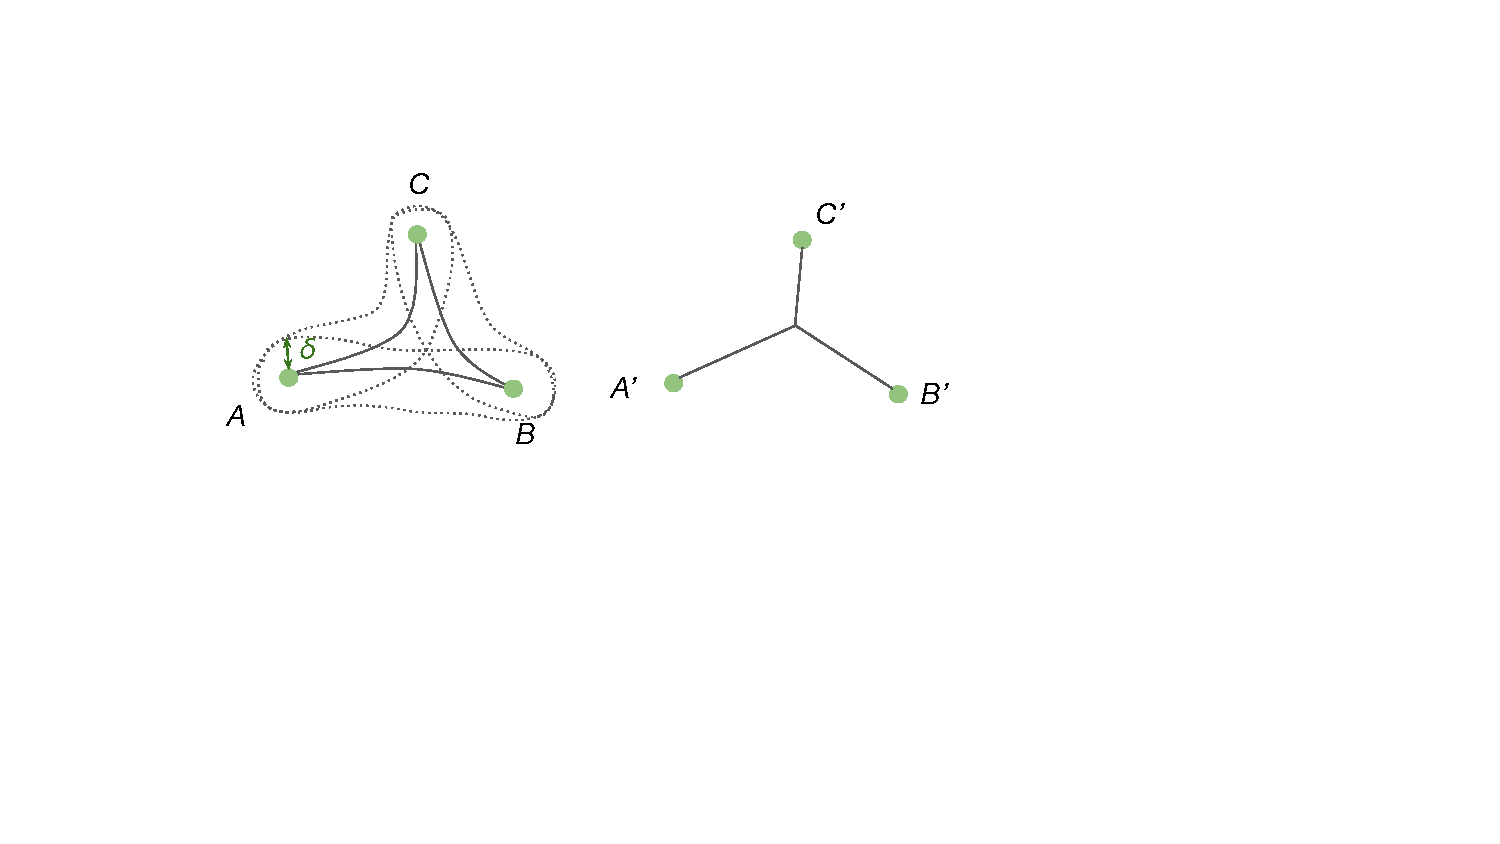
\includegraphics[width=0.5\textwidth]{figures/delta.pdf}
    \caption{Example of a $\delta$-slim triangle, where each side of $\triangle ABC$ is the geodesic distance of two points in the metric space.}
    \label{fig:delta-slim}
\end{figure}


Following \citet{khrulkov2020hyperbolic}, we use the scale-invariant metric $\delta_{rel} = \frac{2\delta}{\text{diam}(\mathcal{X})}$ for evaluation, so that the $\delta_{rel}$ is normalized in $[0,1]$, and the $\text{diam}(\cdot)$ is the set diameter or the maximal pairwise distance.



\section{Additional Experimental Results}
\label{app:secC}


\subsection{Results using Linear Evaluation}
\label{app:sec_linear_evaluation}
We also perform an evaluation of the \emph{fine} classification accuracy following the common linear evaluation protocol \citet{2020supcon} where a linear classifier is trained on top of the normalized penultimate layer features.  We report these accuracies for the models trained on the CIFAR10 and CIFAR100 datasets in \Cref{tab:linear_evals} for the leaf-only variants of the models. We observe that the relative trend of accuracies is identical to the ones reported using the kNN evaluation in Table \ref{tab:combined_metrics_accuracy} and our proposed method \texttt{HypStructure} outperforms the \emph{flat} and $\ell_2$-CPCC methods on both the datasets.

  \begin{table}[t]
  \caption{Linear classification accuracy  using \texttt{SupCon} \citep{2020supcon} as $\ell_\text{Flat}$.}
  \vspace{0.2cm}
    \centering
    \resizebox{0.5\textwidth}{!}{
        \begin{tabular}{lcc}
            \toprule
            \textbf{Dataset} & \textbf{Method (SupCon)} & \textbf{Fine Accuracy ($\uparrow$)} \\
            \midrule
            \multirow{3}{*}{CIFAR10} & Flat & 94.53 \\
            & $\ell_2$-CPCC  & 95.08\\
            & \cellcolor{gray!20}\texttt{HypStructure} (Ours) & \cellcolor{gray!20}\textbf{95.18}\\
            \midrule
            \multirow{3}{*}{CIFAR100} & Flat & 75.11\\
            & $\ell_2$-CPCC  & 75.66\\
            & \cellcolor{gray!20}\texttt{HypStructure} (Ours) & \cellcolor{gray!20}\textbf{77.66}\\
            \bottomrule
        \end{tabular}
    }
    \label{tab:linear_evals}
  \end{table}


\subsection{Component-wise Ablation Study of \texttt{HypStructure}}
\label{app:sec_ablations}


To understand the role of each component in our proposed methodology \texttt{HypStructure}, we perform a detailed ablation study with the different components and measure the \emph{fine} and the \emph{coarse} accuracies on the CIFAR100 dataset. Specifically, we examine

\begin{enumerate}
    \item the role of embedding all internal nodes in the label hierarchy (\cref{eq:objective_hyp} and line 10 in \Cref{alg:hypstructure}), as opposed to only using leaf nodes as in \citet{zeng2022learning}. We refer to the inclusion of internal nodes as $\gT_{\text{int}}$.
    
    \item the role of hyperbolic class centroids computation using hyperbolic averaging (\cref{eq:hypave} and line 8 in \Cref{alg:hypstructure}), as opposed to the Euclidean computation of class prototypes as in \citet{zeng2022learning}. We refer to the hyperbolic class centroid computation as $\omega_{\text{hyp}}$.

    \item the role of the hyperbolic centering loss in our proposed methodology (\cref{eq:objective_hyp} and line 11 in \Cref{alg:hypstructure}), as opposed to not using a centering loss. We refer to the inclusion of the centering loss as $\ell_\text{center}$.
\end{enumerate}



\begin{table}[ht]
\centering
\caption{Ablation study on the components of \texttt{HypStructure}. We report the Classification accuracies based on the CIFAR100 model trained with ResNet-34. 
}
  \vspace{0.2cm}
    \centering
\resizebox{\textwidth}{!}{
\begin{tabular}{ccccc}
\toprule
\multicolumn{3}{c}{\texttt{HypStructure} \textbf{ Components}} & \multicolumn{2}{c}{\textbf{Classification Acc.}$\uparrow$}\\
\cmidrule(lr){1-3} \cmidrule(lr){4-5}
 \textbf{Internal Nodes} ($\gT_{\text{int}}$)     & \textbf{Hyp. Class Centroids} ($\omega_{\text{hyp}}$) & 
 \textbf{Hyp. Centering} ($\ell_\text{center}$)  & \textbf{Fine}  & \textbf{Coarse}\\
\midrule
$\checkmark$ & & & 75.03 & 84.77\\
$\checkmark$ & & $\checkmark$ & 75.61 & 84.81\\
& $\checkmark$ & $\checkmark$ & 76.22 & 85.70\\
$\checkmark$ & $\checkmark$ & & 76.59 & \textbf{86.23}\\
$\checkmark$ & $\checkmark$ & $\checkmark$ & \textbf{76.91} & 86.22\\
            \bottomrule
\end{tabular}
}
\label{tab:ablation_component}
\end{table}



We ablate over the aforementioned settings, where a $\checkmark$ denotes the inclusion of that setting, and report the results on the CIFAR100 dataset in \Cref{tab:ablation_component}. Firstly, we observe that while the centering loss $\ell_\text{center}$ improves the coarse accuracy only by a small increment, it leads to a significant improvement in the fine accuracy (rows $ 1 \rightarrow 2$ and $4 \rightarrow 5$), indicating that the centering of the root in the poincare disk allows for a better relative positioning of the fine classes within the coarse class groups. Secondly, we observe that both the inclusion of internal nodes $\gT_{\text{int}}$, and the hyperbolic computation of the class centroids $\omega_{\text{hyp}}$ is critical for accurately embedding the hierarchy, and removing either of these components (i.e. rows $ 5 \rightarrow 3$ for   $\gT_{\text{int}}$ and rows $ 5 \rightarrow 2$ for $\omega_{\text{hyp}}$), leads to a degradation in both the fine as well as the coarse accuracies.  The best overall performance is observed when all three of the components are included (row $5$).


\subsection{OOD detection}
\label{app:sec_ood_detection}

\subsubsection{Related Work and Methods}
\label{app:ood_citations}
The goal of prior works in the OOD literature is the supervised setting of learning an accurate classifier for ID data, along with an ID-OOD detection methodology and this task has been explored in the generative model setting \citep{kirichenko2020normalizing,nalisnick2019deep,ren2019likelihood,serra2019input,xiao2020likelihood}, and more extensively in the supervised discriminative model setting \citep{openmax16cvpr,hendrycks2016baseline,hsu2020generalized,huang2021mos,liang2018enhancing,liu2020energy,sun2021tone,ming22a}. The methods in this setting can be categorized into four sub-categories following \citep{zhang2023openood}, primarily:

\paragraph{Post-Hoc Inference} These methods design post-processing/scoring mechanisms on base classifiers such as MSP \citep{hendrycks2016baseline}, ODIN \citep{liang2018enhancing}, ReAct \citep{sun2021tone}, SSD+ \citep{2021ssd}, KNN+ \citep{sun2022knnood} and RankFeat \citep{song2022rankfeat}. 
\paragraph{Training without outlier data} These methods involve training-time regularization or different objective functions for improving OOD detection capabilities such as G-ODIN \citep{hsu2020generalized}, CSI \citep{tack2020csi}, LogitNorm \citep{wei2022mitigating} and CIDER \citep{cider2022ming}. 

\paragraph{Training with outlier data} These methods assume access to auxiliary OOD training samples such as OE \citep{oe18nips} and MixOE \citep{mixoe23wacv}. 

\paragraph{Data Augmentation} These methods improve the generalization ability of image classifiers such as StyleAugment \citep{geirhos2018imagenettrained}, AugMix \citep{hendrycks2020augmix} and RegMixup \citep{pinto2022using}. \\

Our proposed work can be considered primarily in the \textbf{Training without outlier data} category, and we note that none of the prior works use any additional structural regularization term in the objective functions.

\subsubsection{Dataset-wise OOD Detection Results}

\begin{table*}[ht]
\caption{Results on CIFAR10. OOD detection performance for {ResNet-18} trained on CIFAR10. Training with \texttt{HypStructure} achieves strong OOD detection performance.}
\centering
\resizebox{0.8\textwidth}{!}{
\begin{tabular}{lccccccccc}
\toprule
\multirow{2}{*}{\textbf{Method}} & \multicolumn{5}{c}{\textbf{OOD Dataset AUROC (↑)}} & \multirow{2}{*}{\textbf{Avg. (↑)}} \\
\cmidrule(lr){2-6} 
& SVHN & Textures & Places365 & LSUN & iSUN & \\
\midrule
ProxyAnchor & 94.55 & 93.16 & 92.06 & 97.02 & 96.56 & 94.67 \\
CE + SimCLR & 99.22 & 96.56 & 86.70 & 85.60 & 86.78 & 90.97 \\
CSI & 94.69 & 94.87 & 93.04 & 97.93 & 98.01 & 95.71 \\
CIDER & 99.72 & 96.85 & 94.09 & 99.01 & \textbf{96.64} & 97.26 \\
\midrule
SSD+ & 99.51 & 98.35 & \textbf{95.57} & 97.83 & 95.67 & 97.38 \\
KNN+ & 99.61 & 97.43 & 94.88 & 98.01 & 96.21 & 97.22  \\
$\ell_2$-CPCC & 93.27 & 94.76 & 60.15 & 75.29 & 59.87 & 76.67 \\
\rowcolor{gray!20}\texttt{HypStructure} (Ours) & \textbf{99.75} & \textbf{98.89} & 94.80 & \textbf{99.67} & 95.64 & \textbf{97.75} \\
\bottomrule
\end{tabular}
}
\label{tab:main_c10_ood}
\end{table*}


\begin{table*}[ht]
\caption{Results on ImageNet100. OOD detection performance for {ResNet-34} trained on ImageNet100. Training with \texttt{HypStructure} achieves strong OOD detection performance.}
\centering
\resizebox{0.8\textwidth}{!}{
\begin{tabular}{lcccccccc}
\toprule
\multirow{2}{*}{\textbf{Method}} & \multicolumn{4}{c}{\textbf{OOD Dataset AUROC (↑)}} & \multirow{2}{*}{\textbf{Avg. (↑)}} \\
\cmidrule(lr){2-5} 
& SUN & Places365 & Textures & iNaturalist & &\\
\midrule
CIDER & 91.63 & 89.29 & 97.98 & 96.35 & 93.81  \\
\midrule
SSD+ & 88.97 & 85.98 & \textbf{98.49} & 96.42 & 92.46 \\
KNN+ & 89.48 & 86.64 & 98.38 & \textbf{96.46} & 92.74 \\
$\ell_2$-CPCC & 90.95 & 86.87 & 97.41 & 90.08 & 91.33 \\
\rowcolor{gray!20}\texttt{HypStructure} (Ours) & \textbf{92.21} & \textbf{90.12} & 97.33 & 95.61 & \textbf{93.83}  \\
\bottomrule
\end{tabular}
}
\label{tab:main_im10_ood}
\end{table*}


We report the dataset-wise OOD detection results in Tables \ref{tab:ood_detection_main_cifar100}, \ref{tab:main_c10_ood} and \ref{tab:main_im10_ood} for CIFAR100, CIFAR10 and ImageNet100 respectively. 
We compare with several other state-of-the-art baseline OOD detection methods for CIFAR10 and CIFAR100, namely ProxyAnchor \citep{kim2020proxy}, SimCLR \citep{chen2020simple} CSI \citep{tack2020csi}, and CIDER \citep{cider2022ming} respectively. Results for these methods are taken from CIDER \citep{cider2022ming} where contrastive learning based OOD detection methods typically outperforms non-contrastive learning ones. For ImageNet100, in the absence of the available class ids used to train the original models in CIDER \citep{cider2022ming}, we finetune the ResNet34 models on the created ImageNet100 dataset. For CIDER and SupCon, we use the official implementations and hyperparameters provided by the authors. 

We observe that our proposed method leads to an improvement in the average OOD detection AUROC over all the ID datasets. In practice, we find that the Euclidean-centroid computational variant (first compute the Euclidean centroids and then apply the exponential map) of our proposed method performs slightly better than the hyperbolic-centroid computational variant (first apply the exponential map and then compute the hyperbolic average), for the specific task of OOD detection, while having equivalent performance on the ID classification task. Hence, we report the OOD detection accuracy corresponding to the first version. 


\subsection{Visualization of Learned Features}
\label{app:sec_add_hyperbolic_viz}

We provide additional visualizations of the learnt features from our proposed method \texttt{HypStructure} on the CIFAR10, CIFAR100 and ImageNet100 datasets in Figures \ref{fig:add_viz_1}, \ref{fig:add_viz_2} and \ref{fig:add_viz_3} respectively. 

\begin{figure}[ht]
\centering
\begin{tabular}{cc}
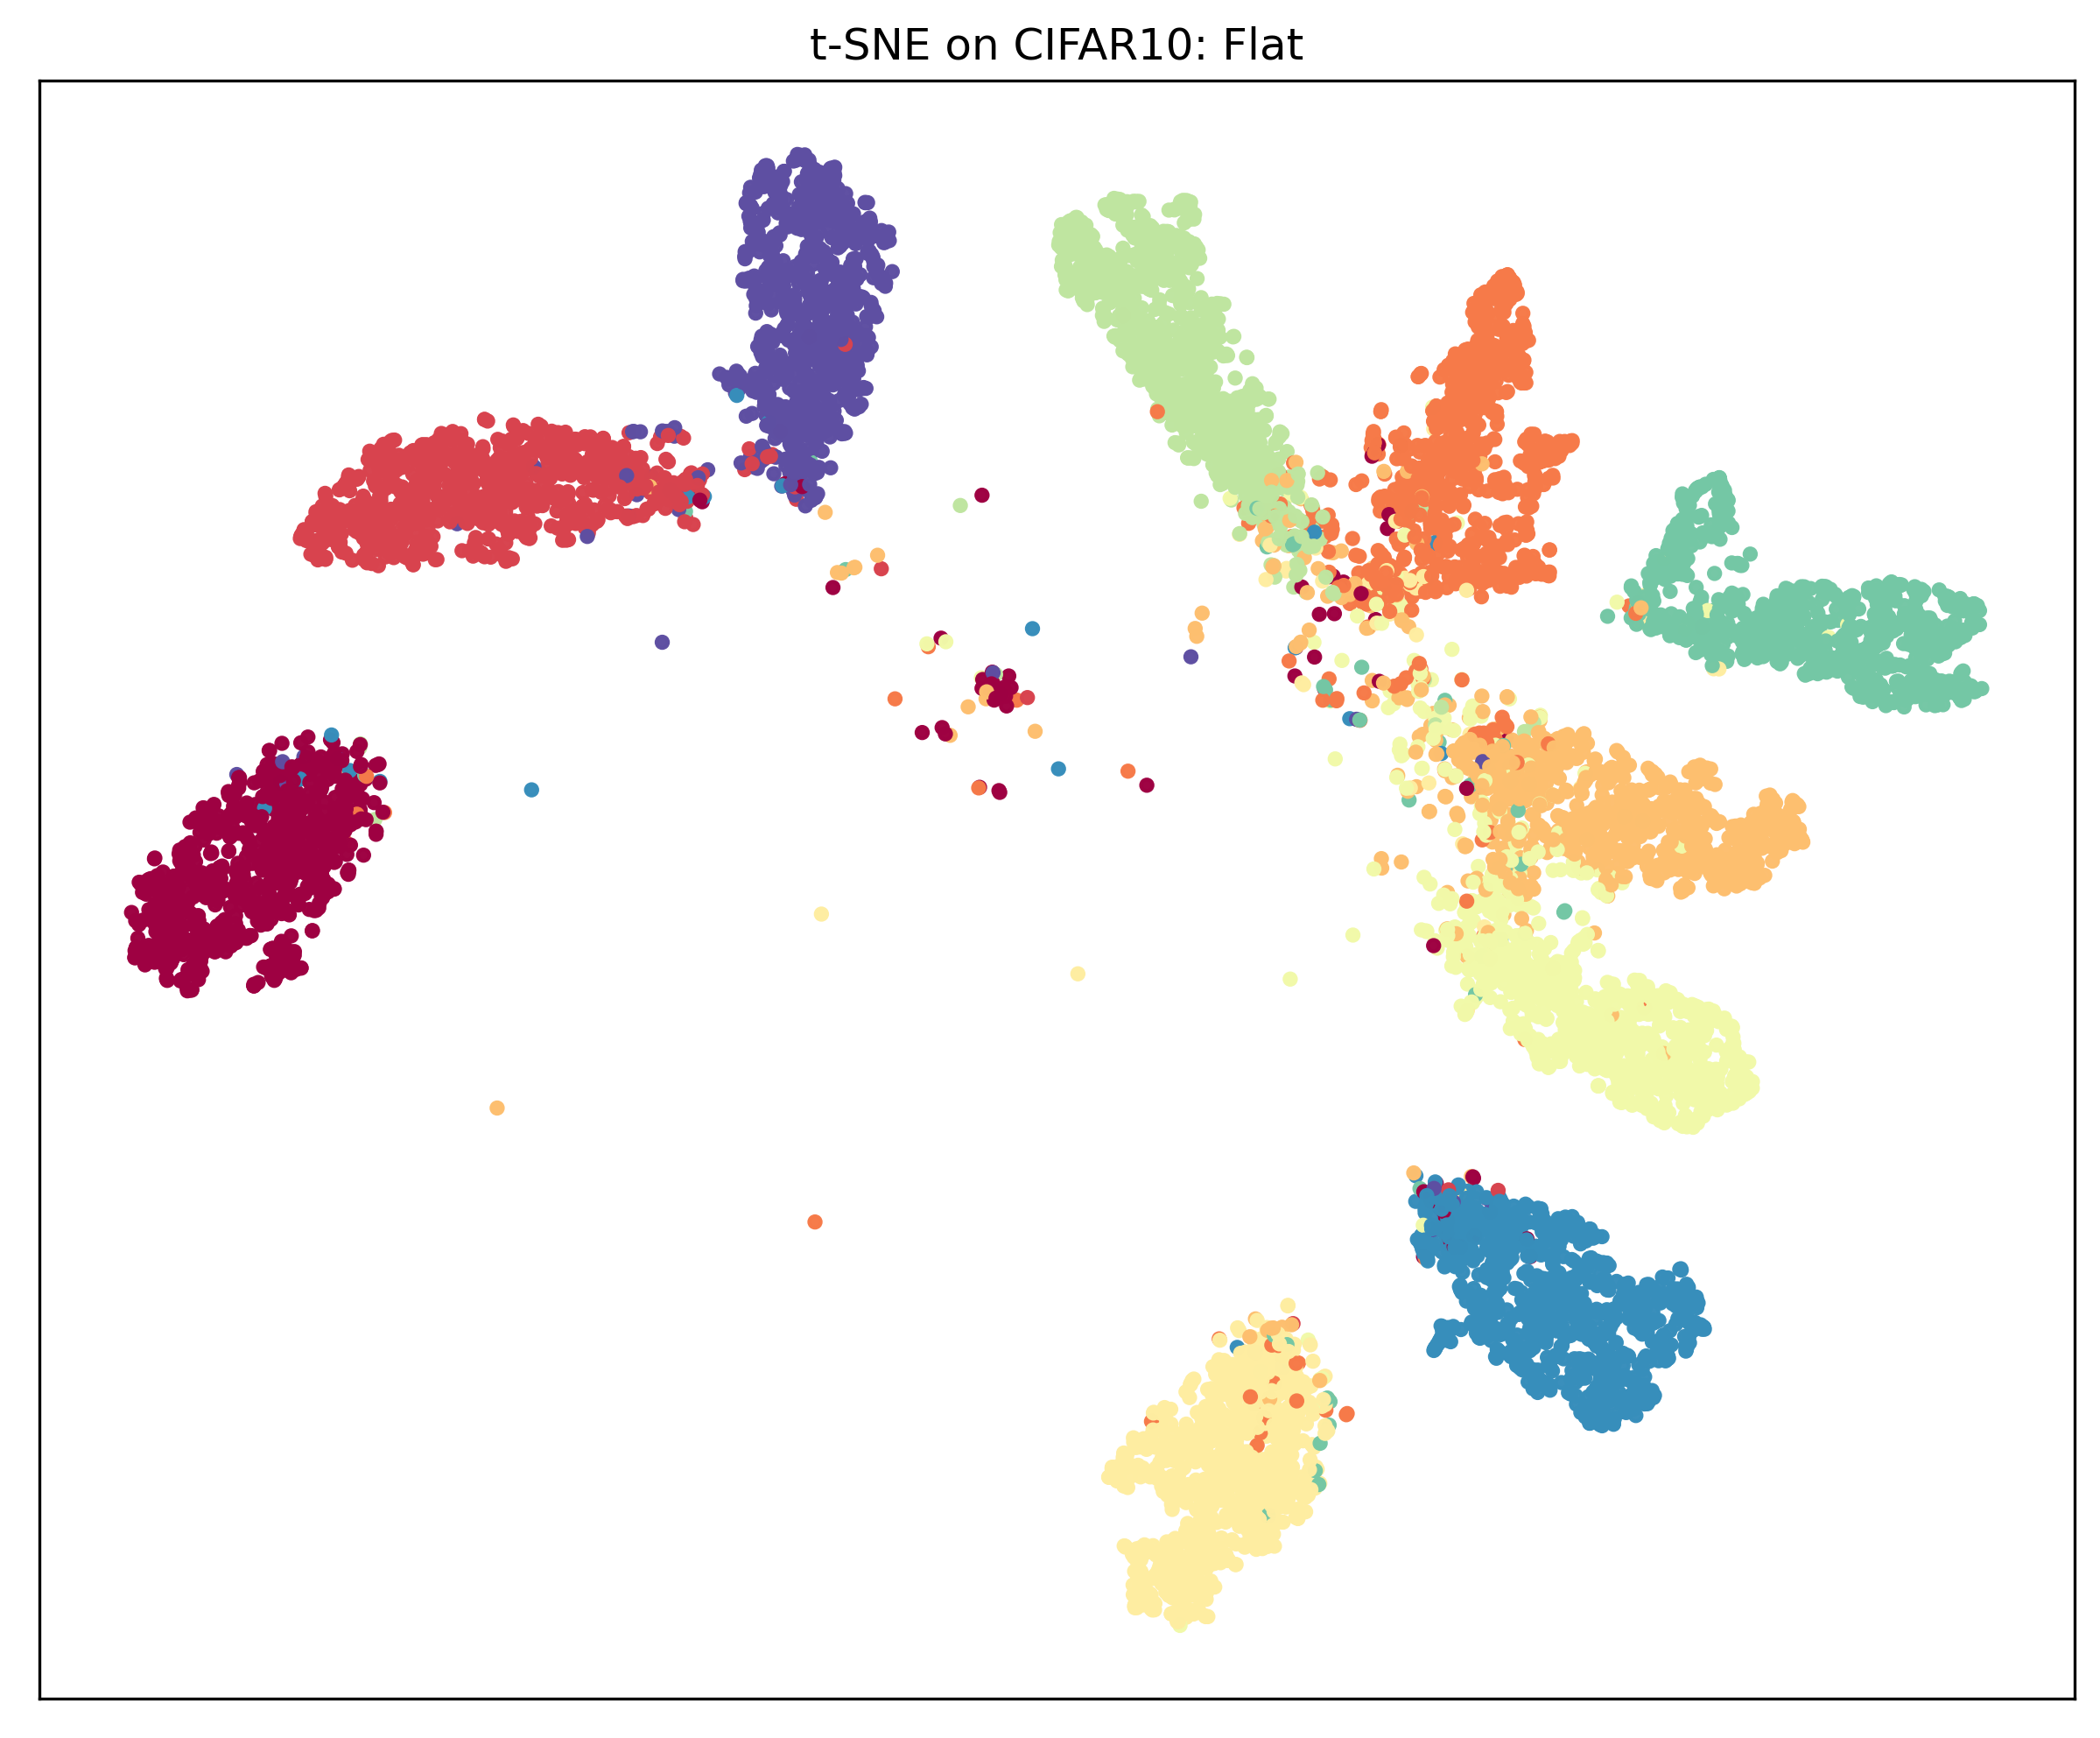
\includegraphics[width=.3\textwidth]{figures/cifar10_tsne_flat.png}&
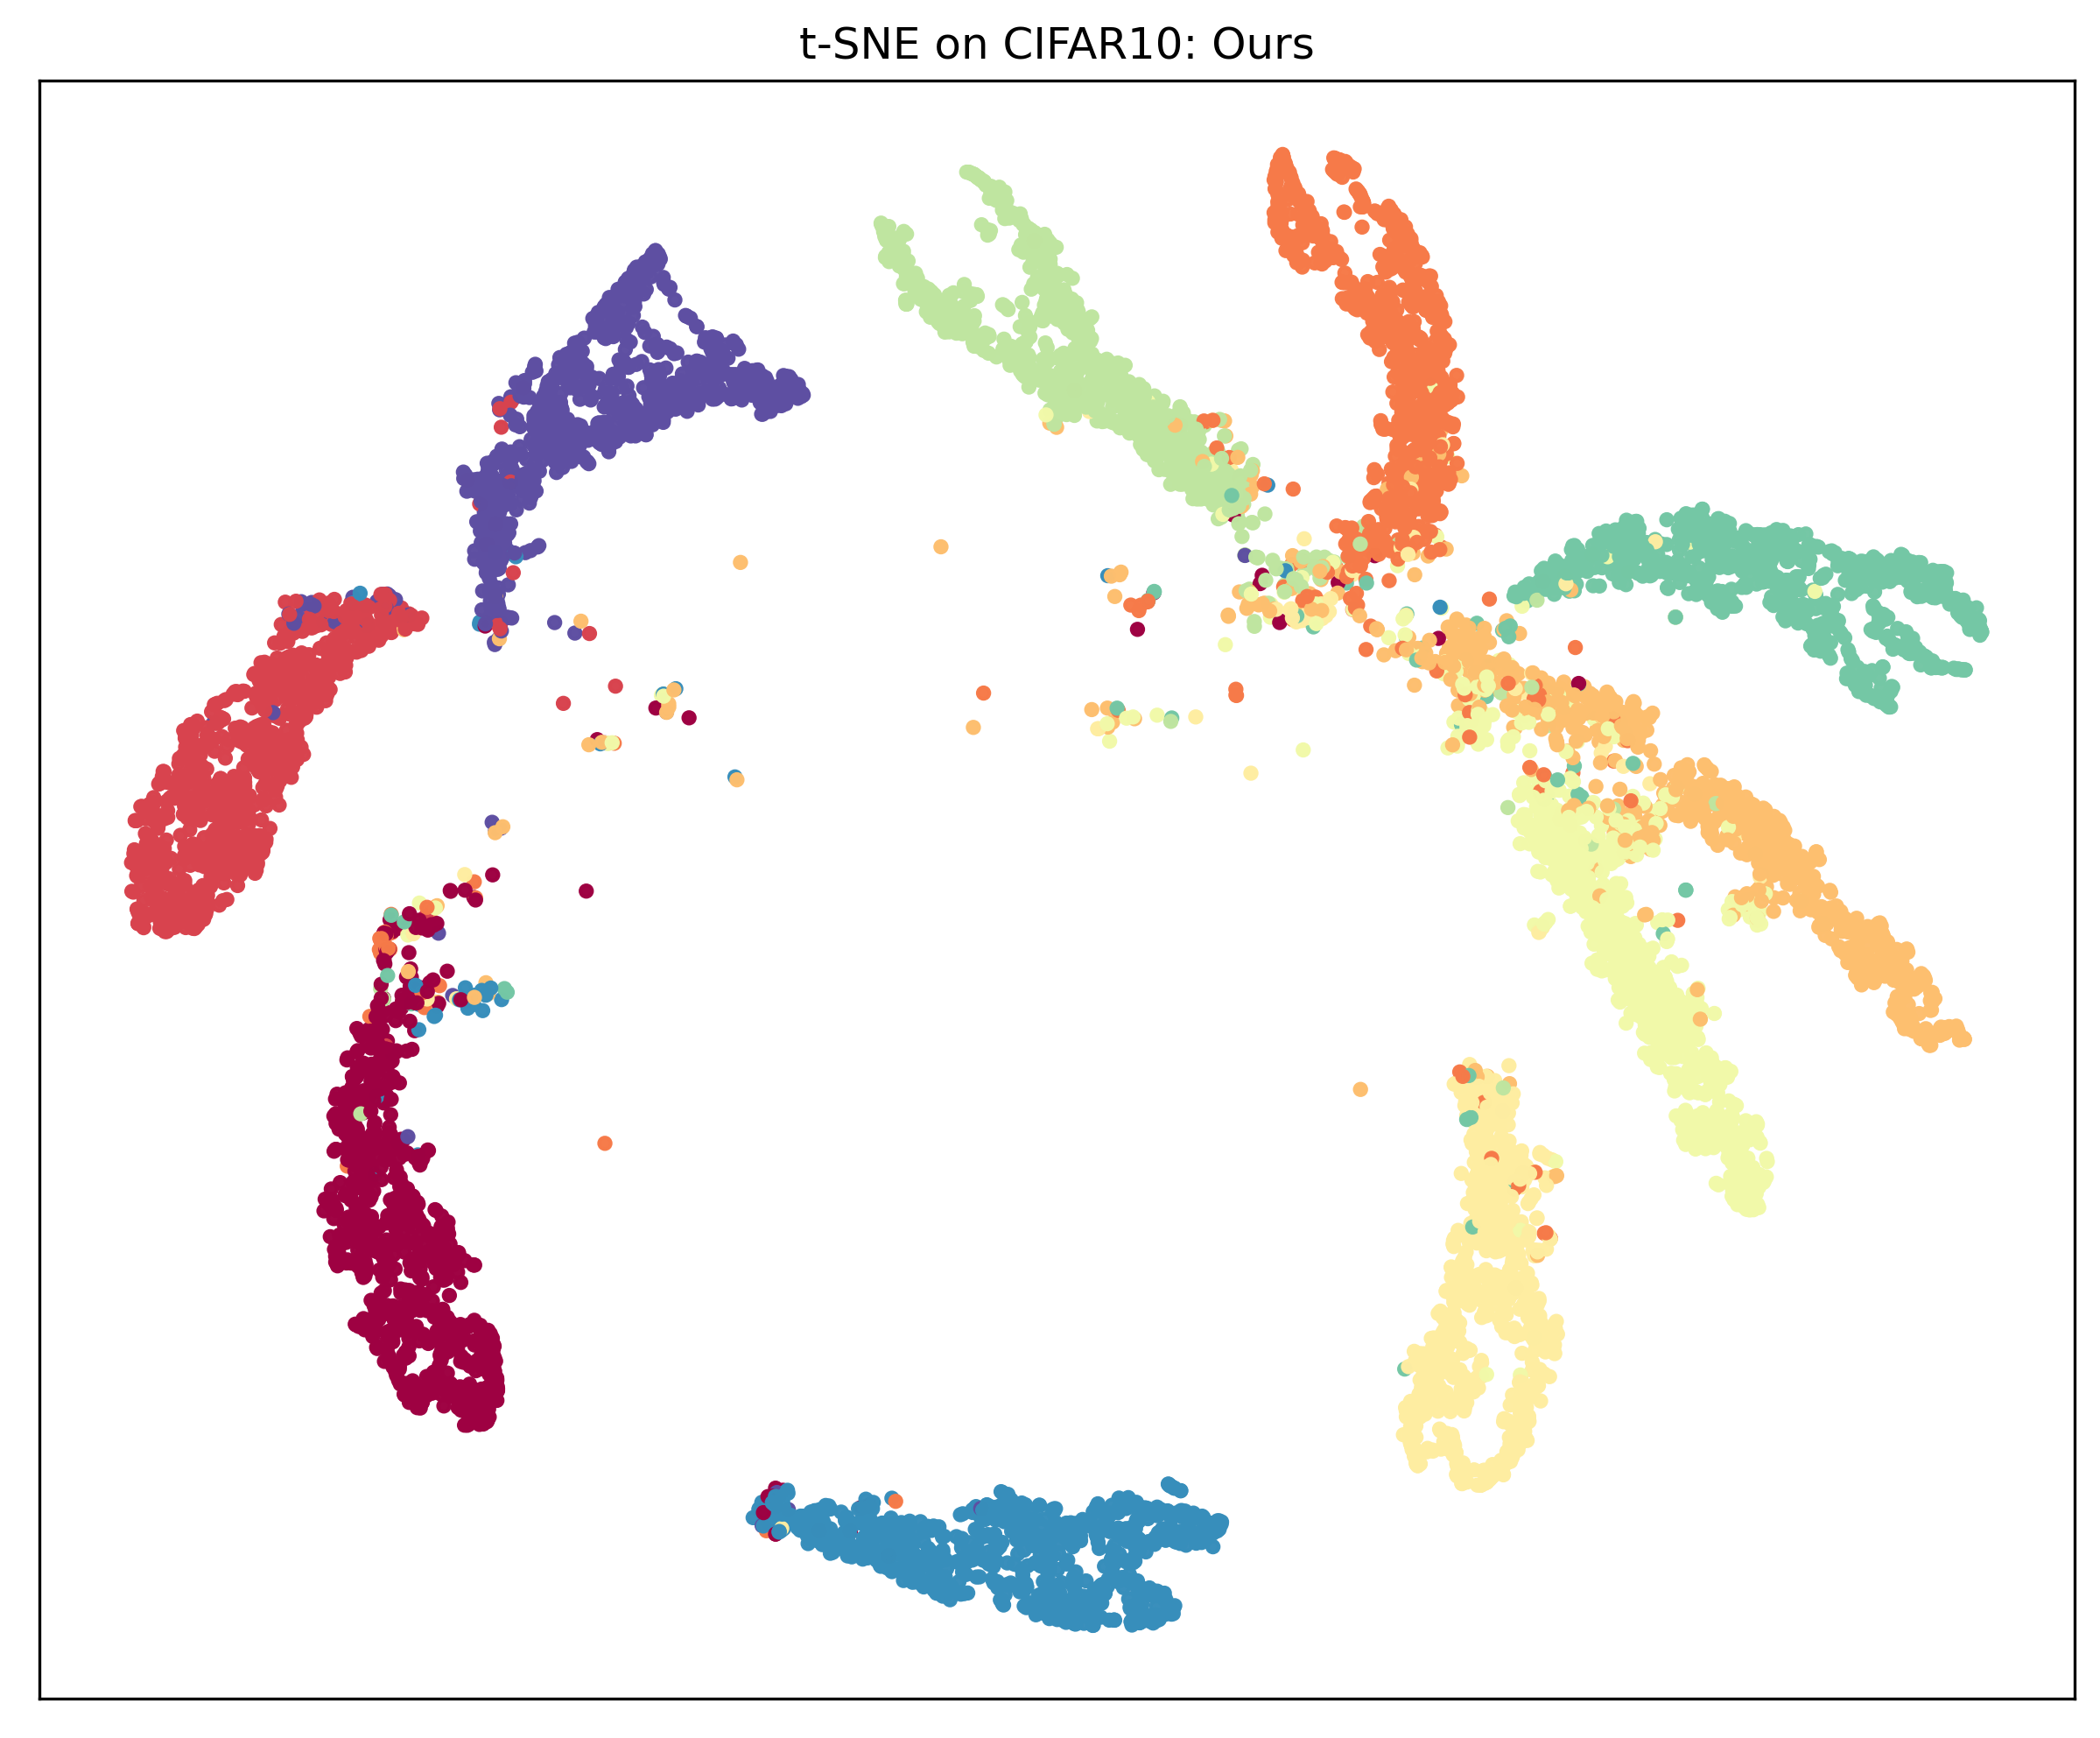
\includegraphics[width=.3\textwidth]{figures/cifar10_tsne_ours.png}\\
{ (a)}&{ (b)} 
\end{tabular}
\caption{Euclidean t-SNE Visualizations on CIFAR10.}
\label{fig:add_viz_1}
\end{figure}


\begin{figure}[ht]
\centering
\begin{tabular}{cc}
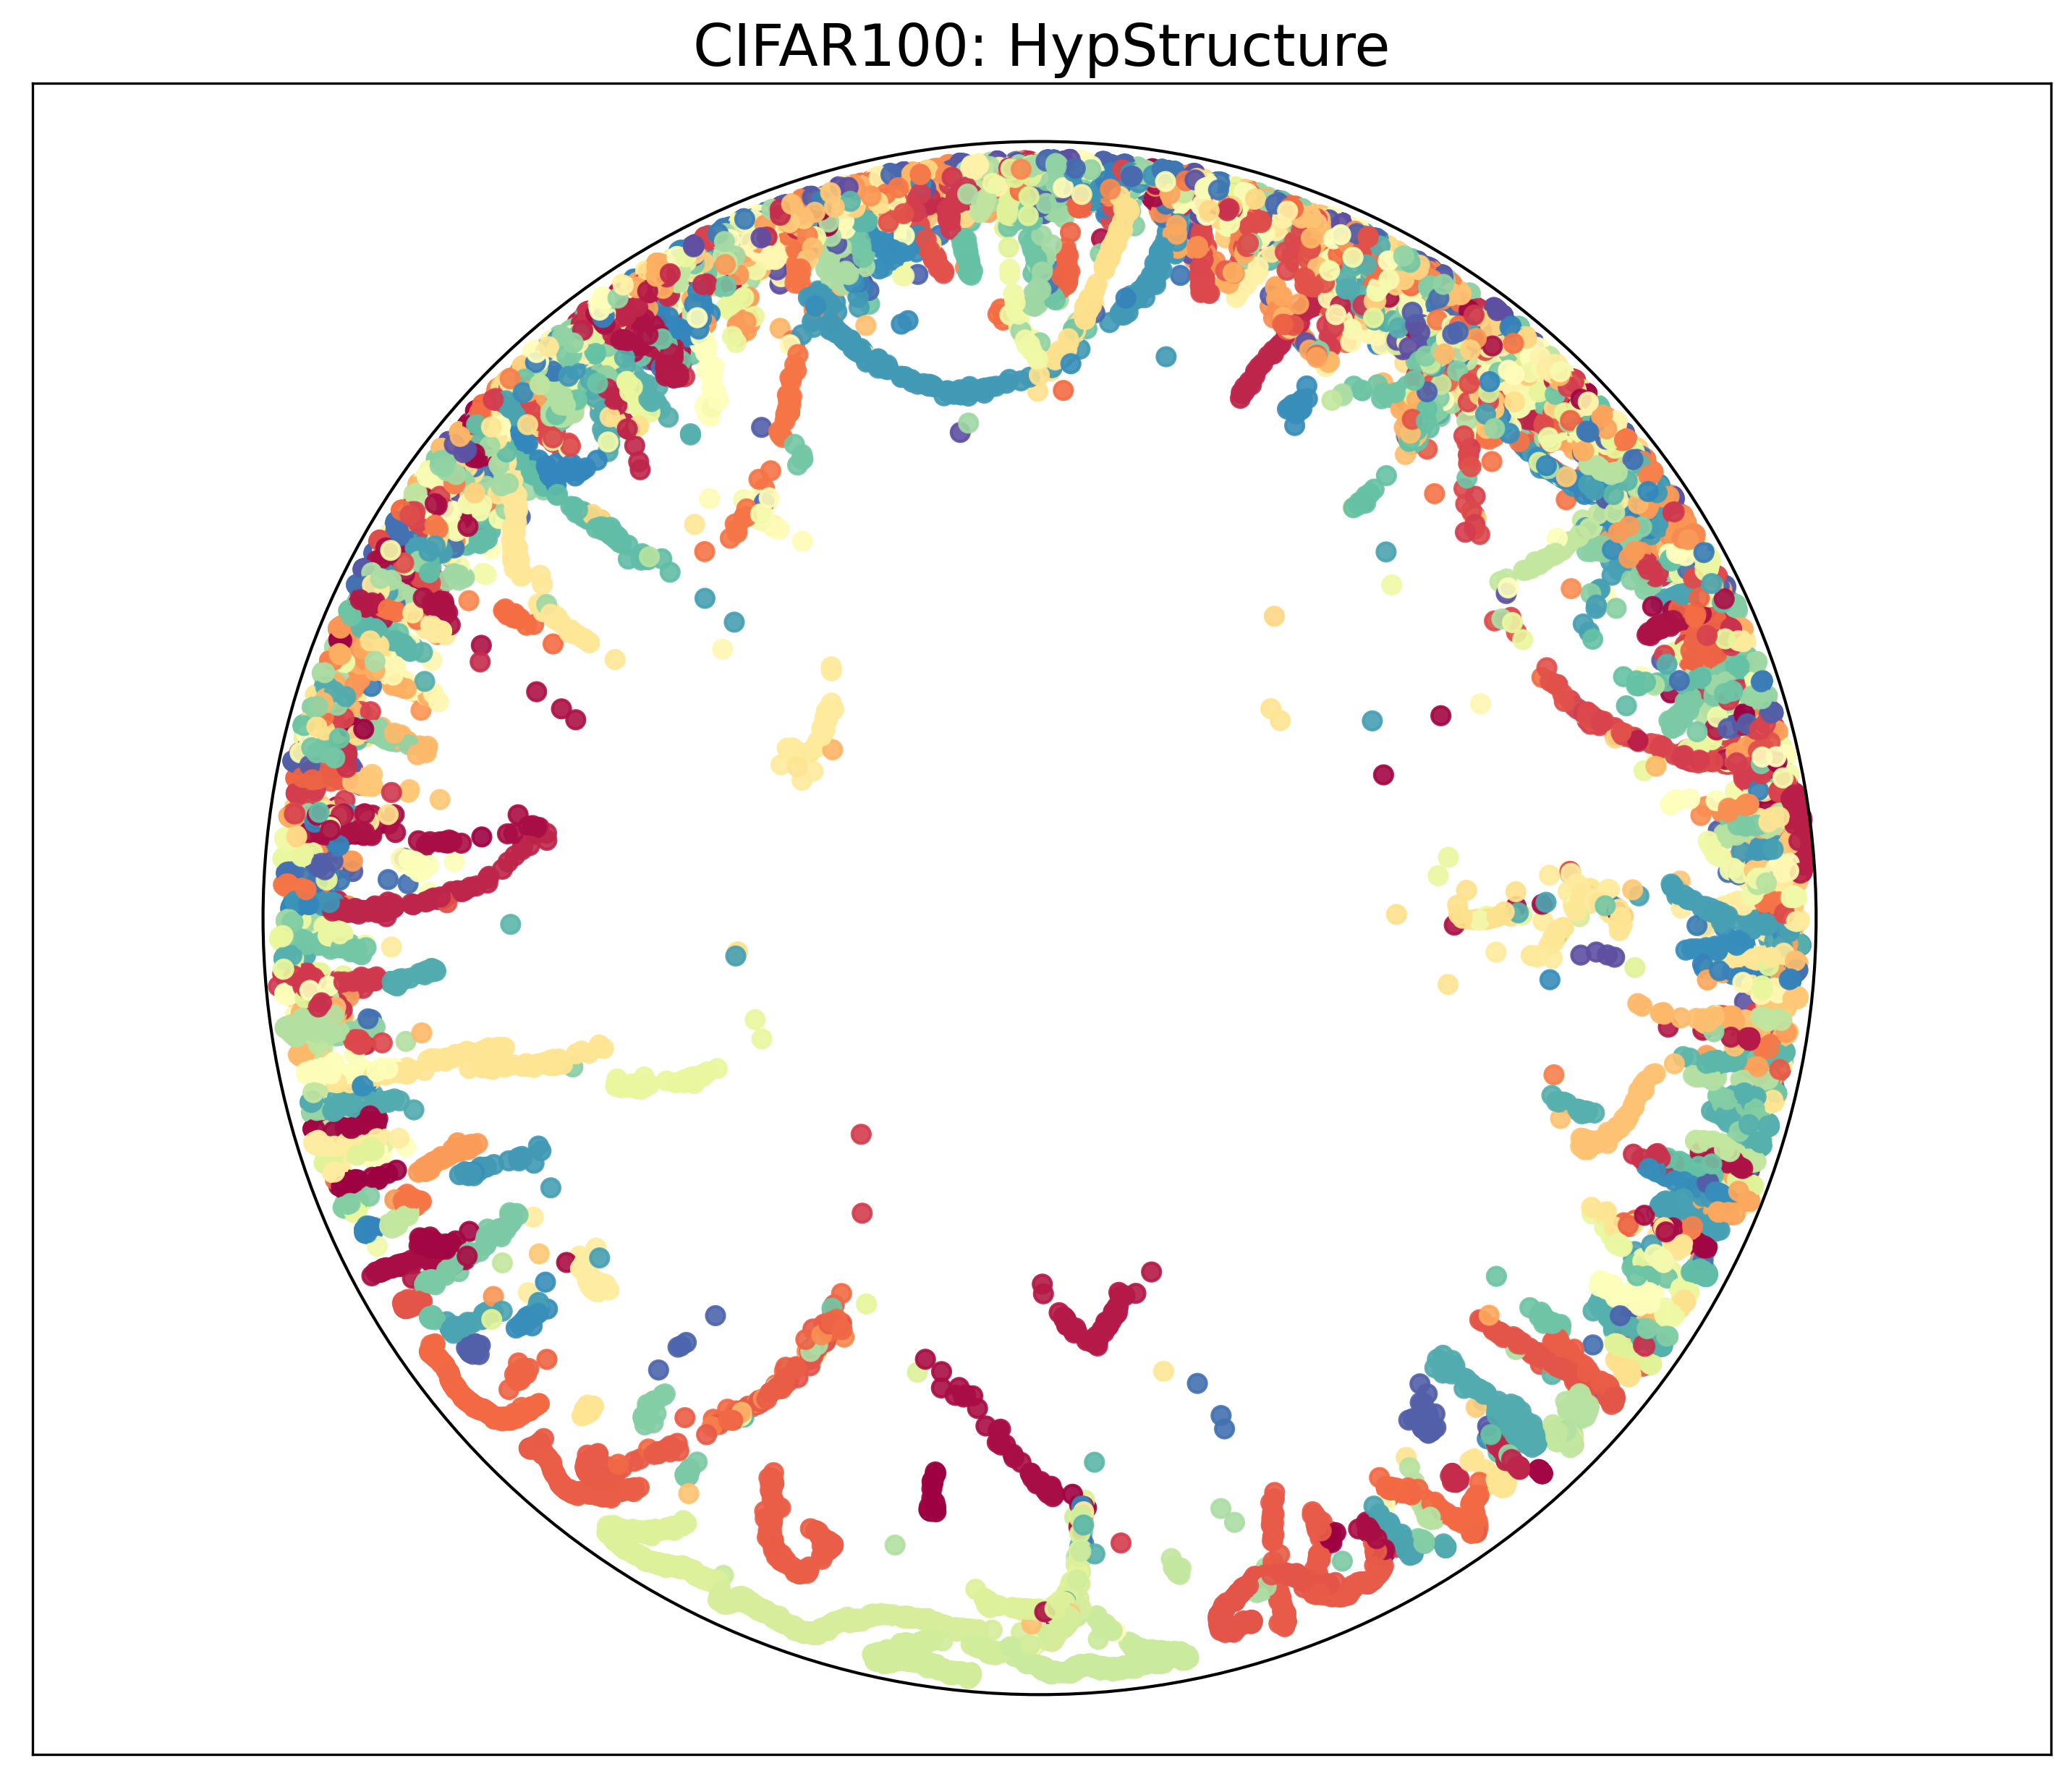
\includegraphics[width=.3\textwidth]{figures/hypstructure_poincare_disk_cifar100.png}&
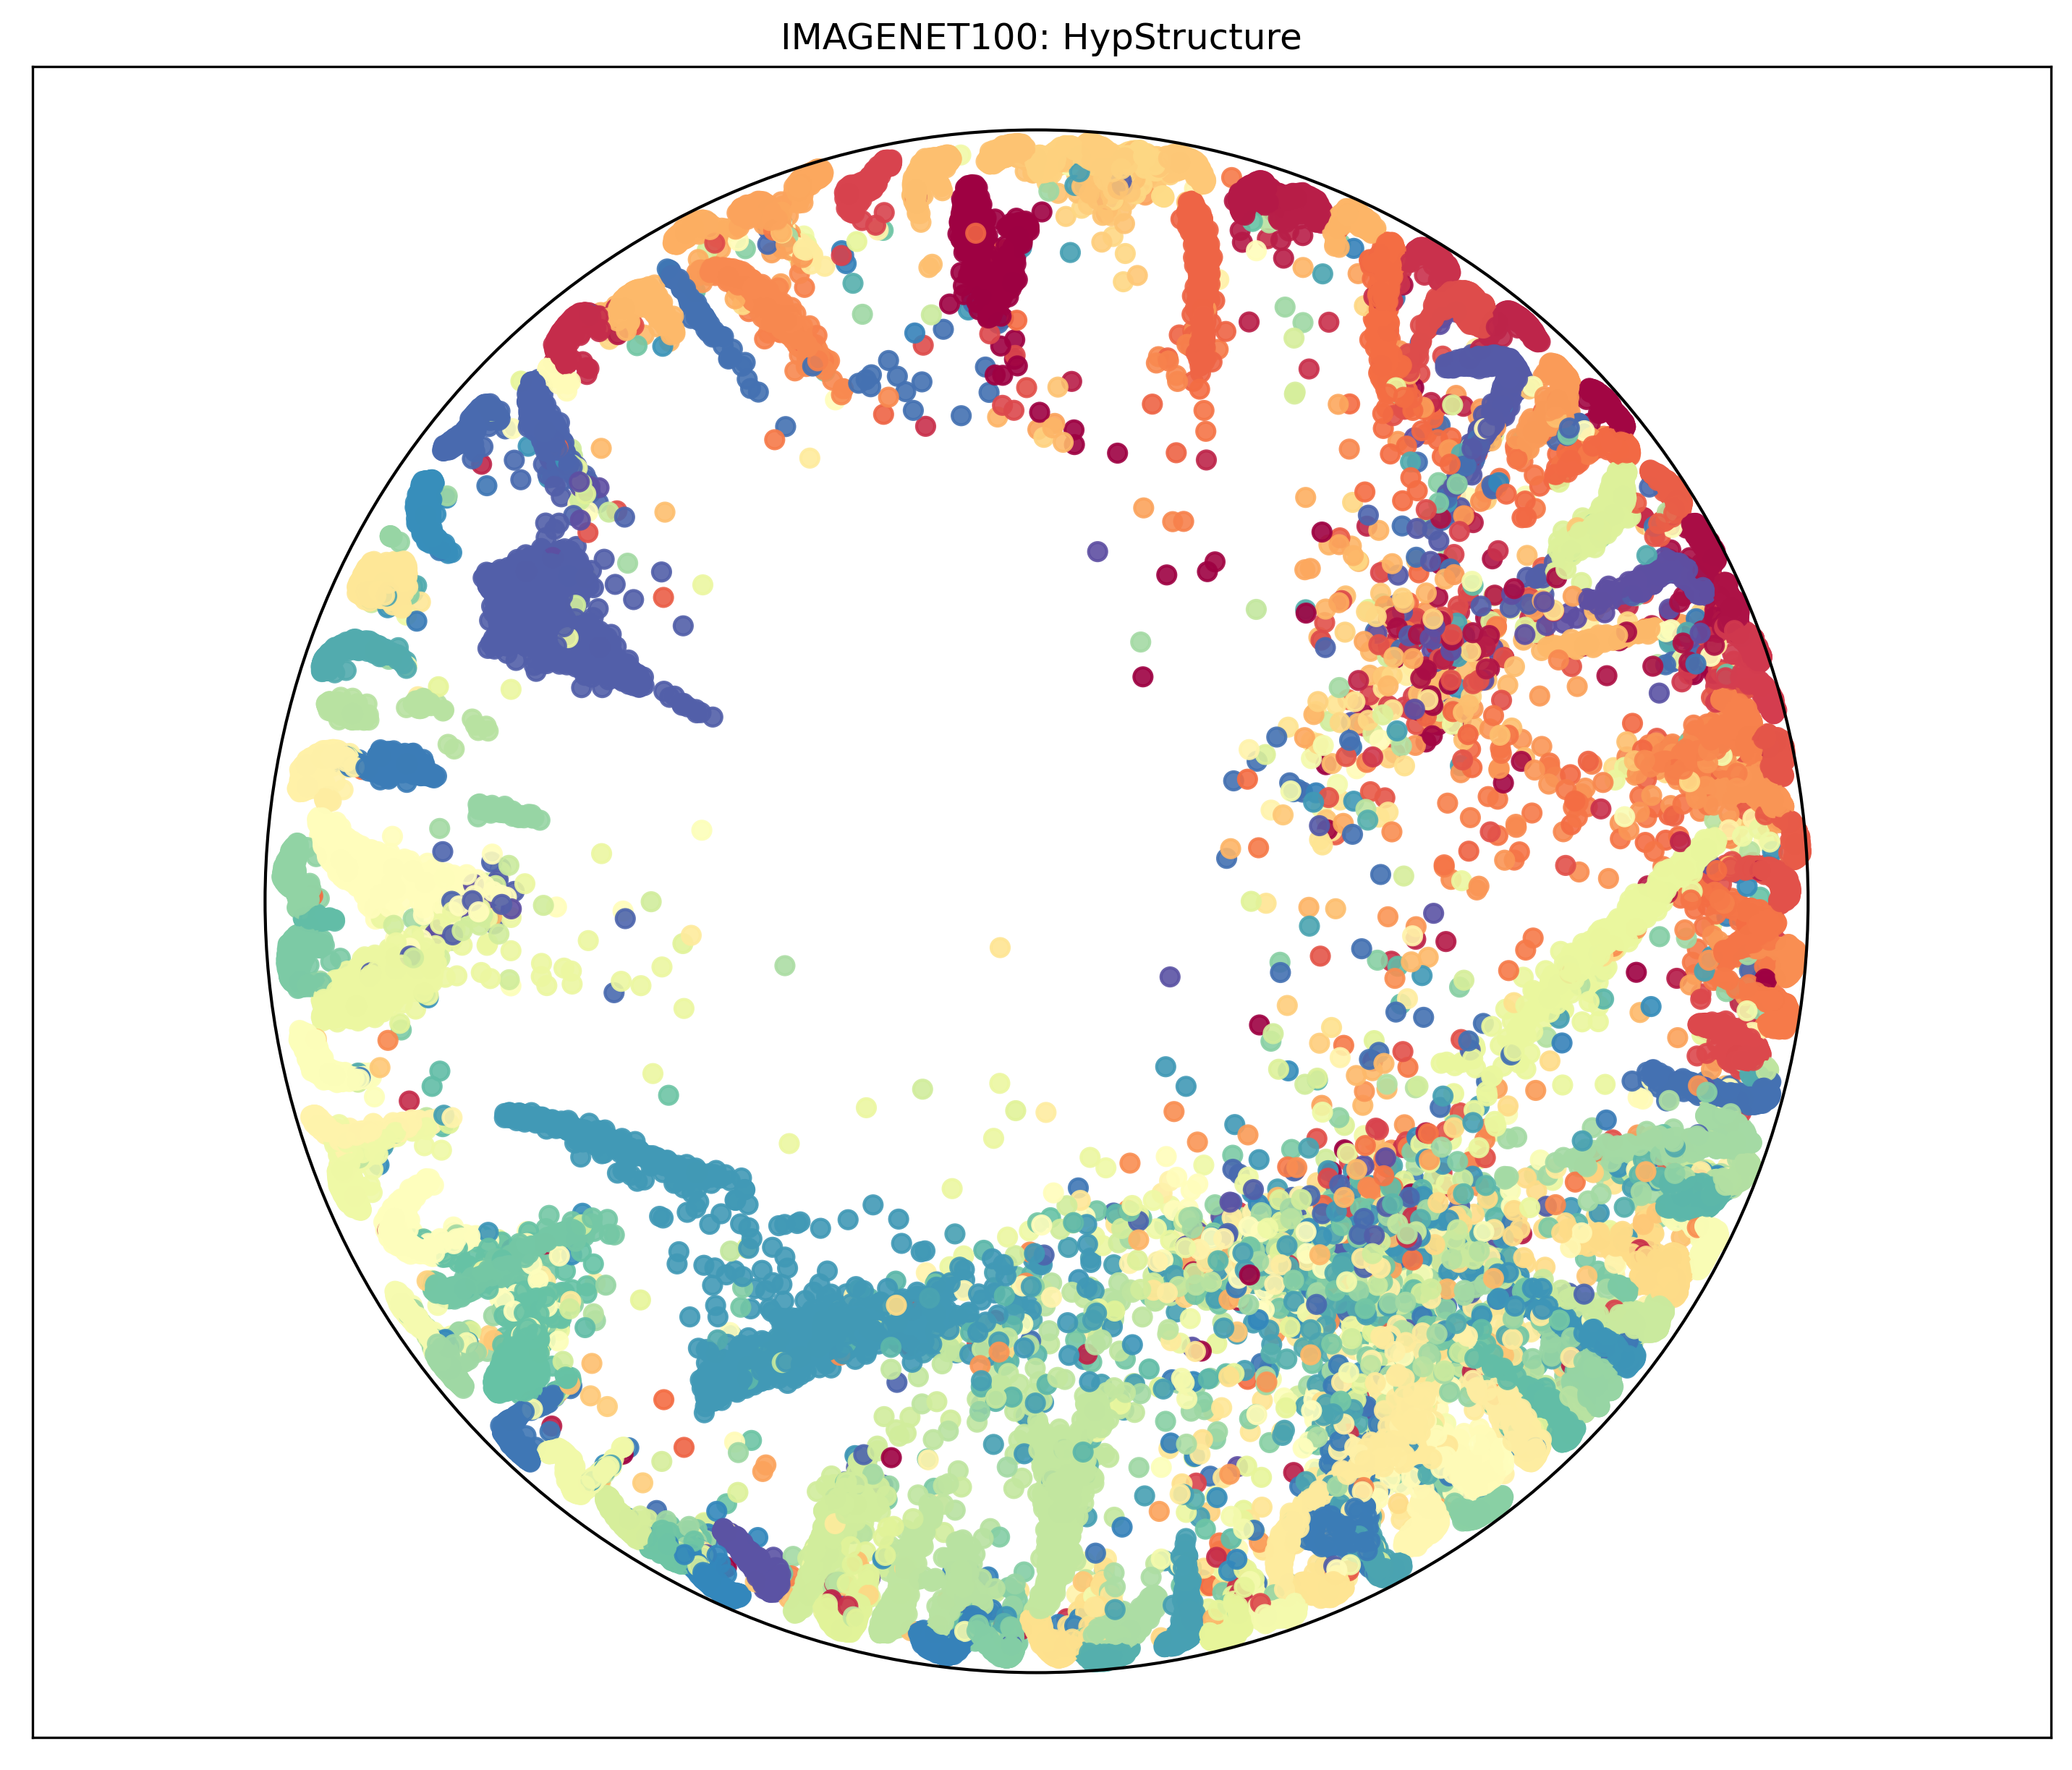
\includegraphics[width=.3\textwidth]{figures/hypstructure_poincare_disk_imagenet100.png}\\
{ (a)}&{ (b)} 
\end{tabular}
\caption{Hyperbolic UMAP Visualizations on CIFAR100 and ImageNet100.}
\label{fig:add_viz_2}
\end{figure}

\begin{figure}[ht]
\centering
\begin{tabular}{cc}
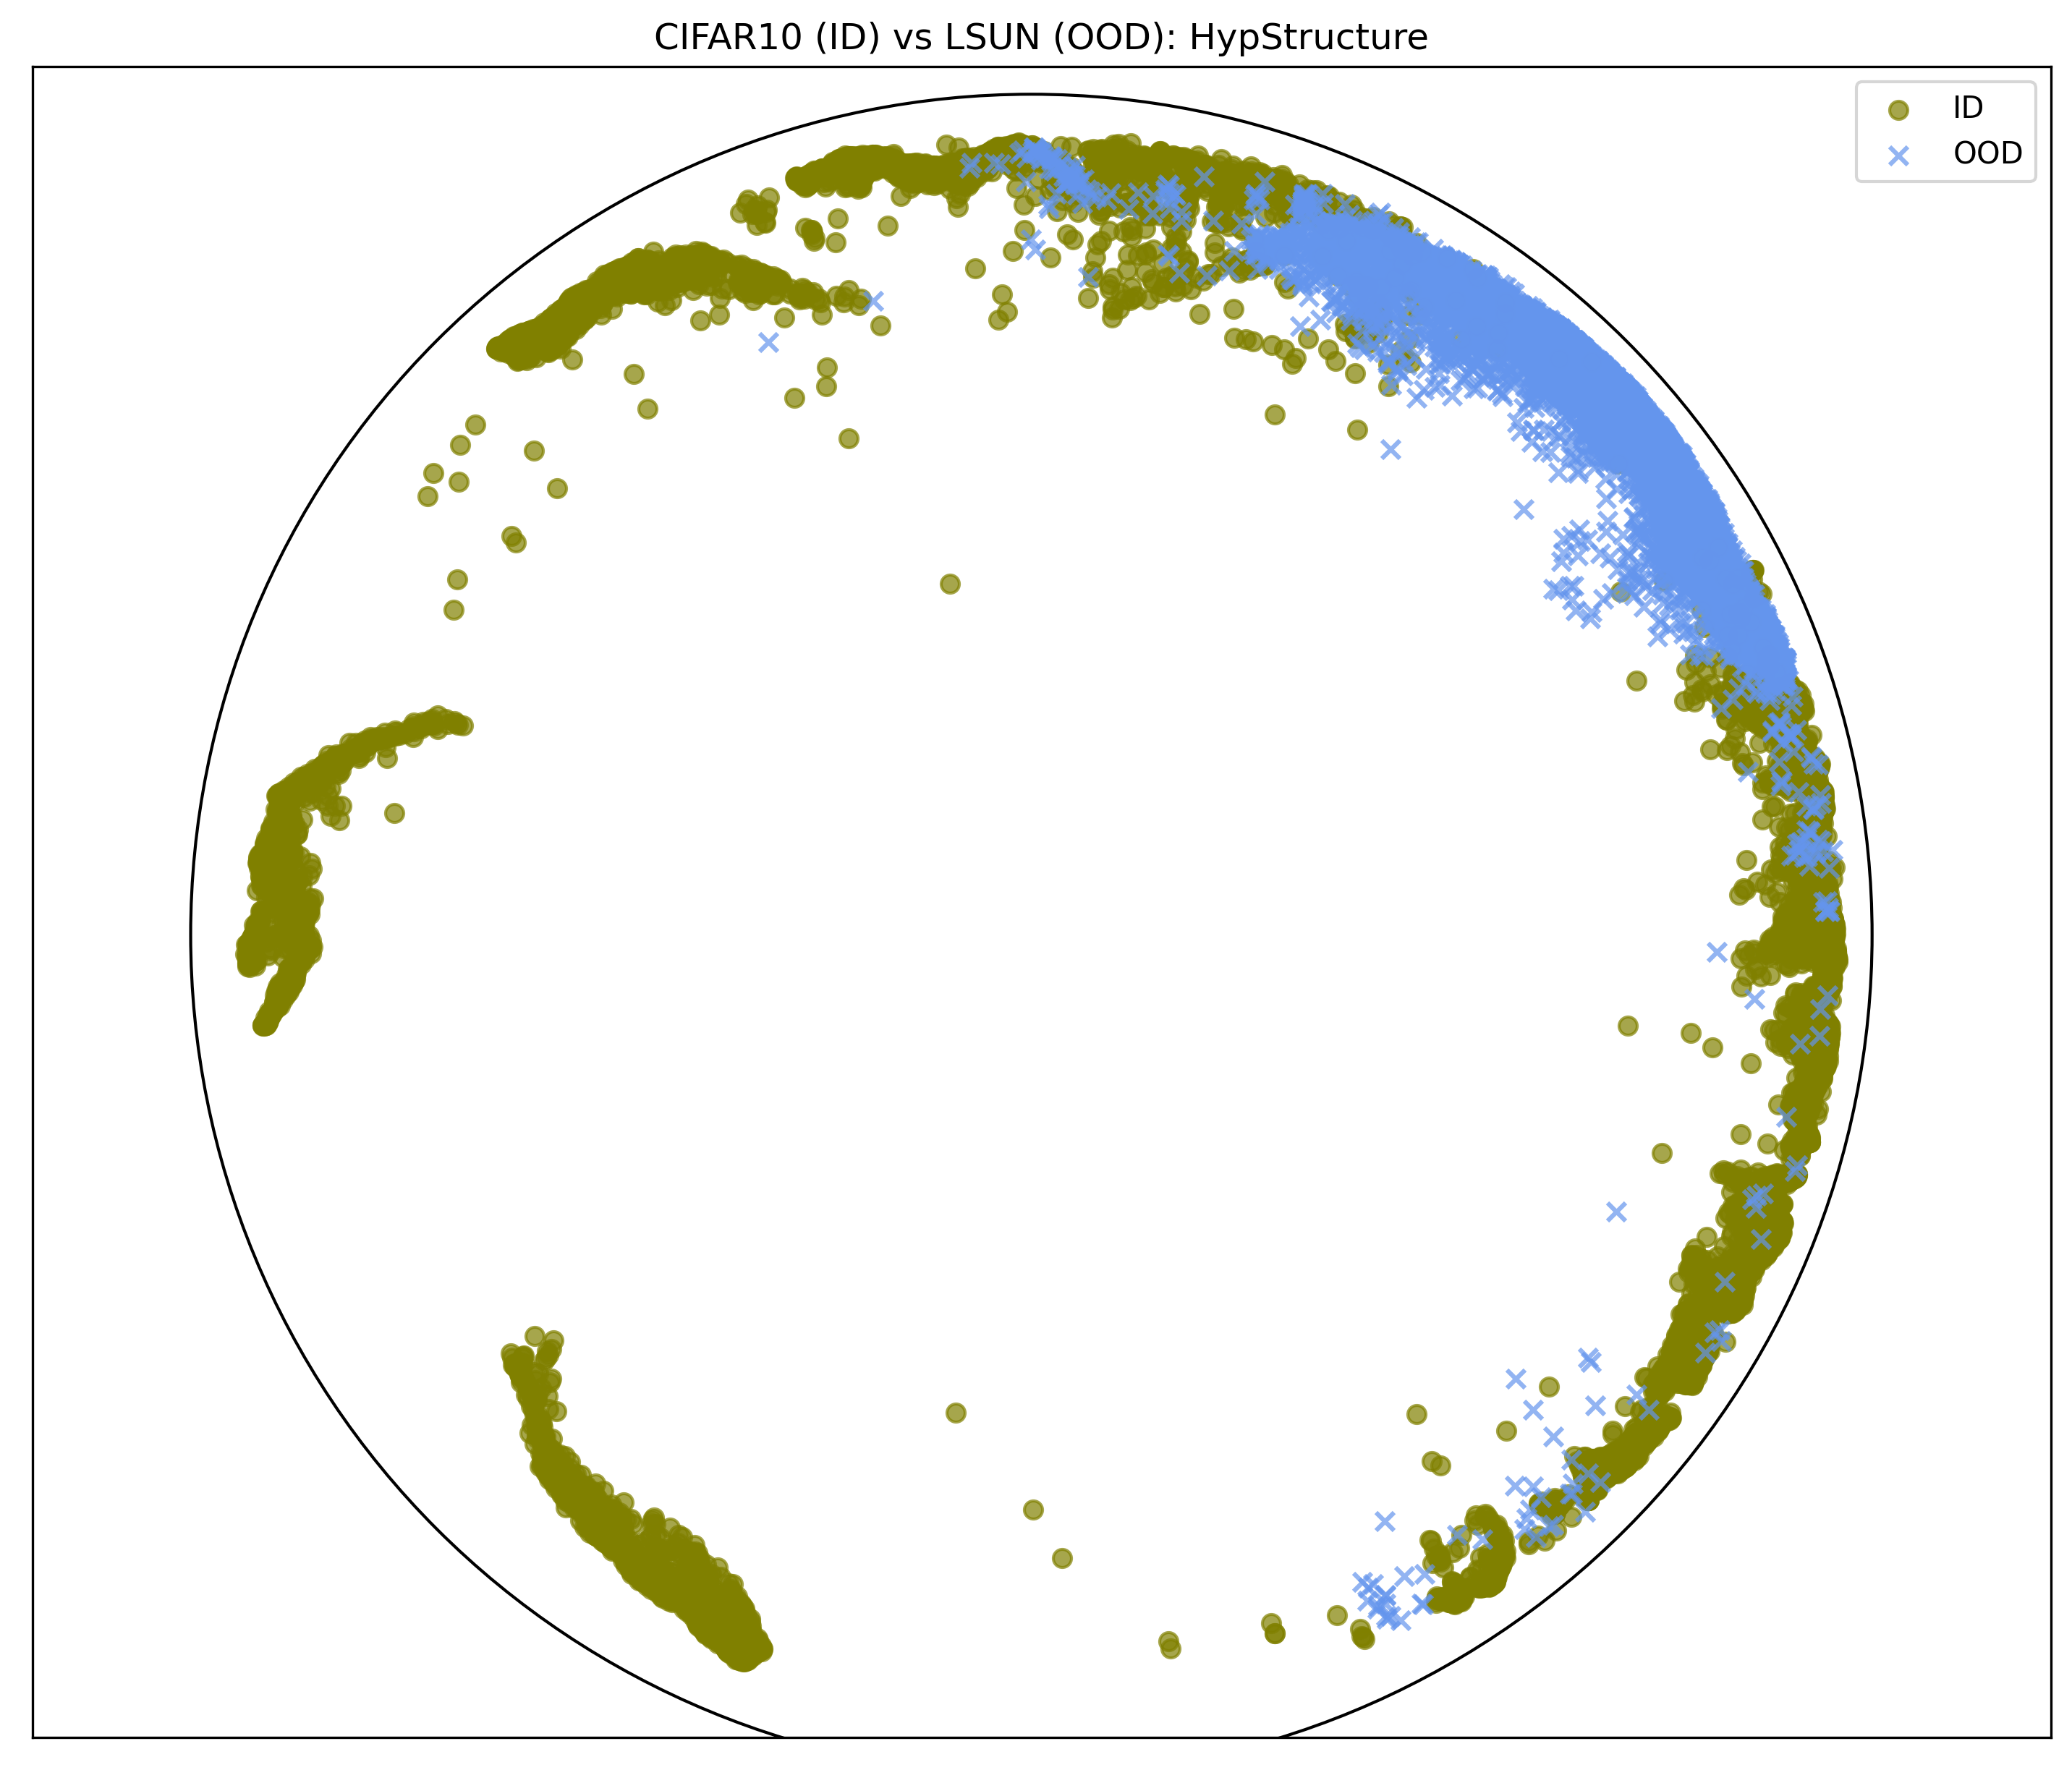
\includegraphics[width=.3\textwidth]{figures/hypstructure_cifar10_poincare_disk_ID_OOD.png}&
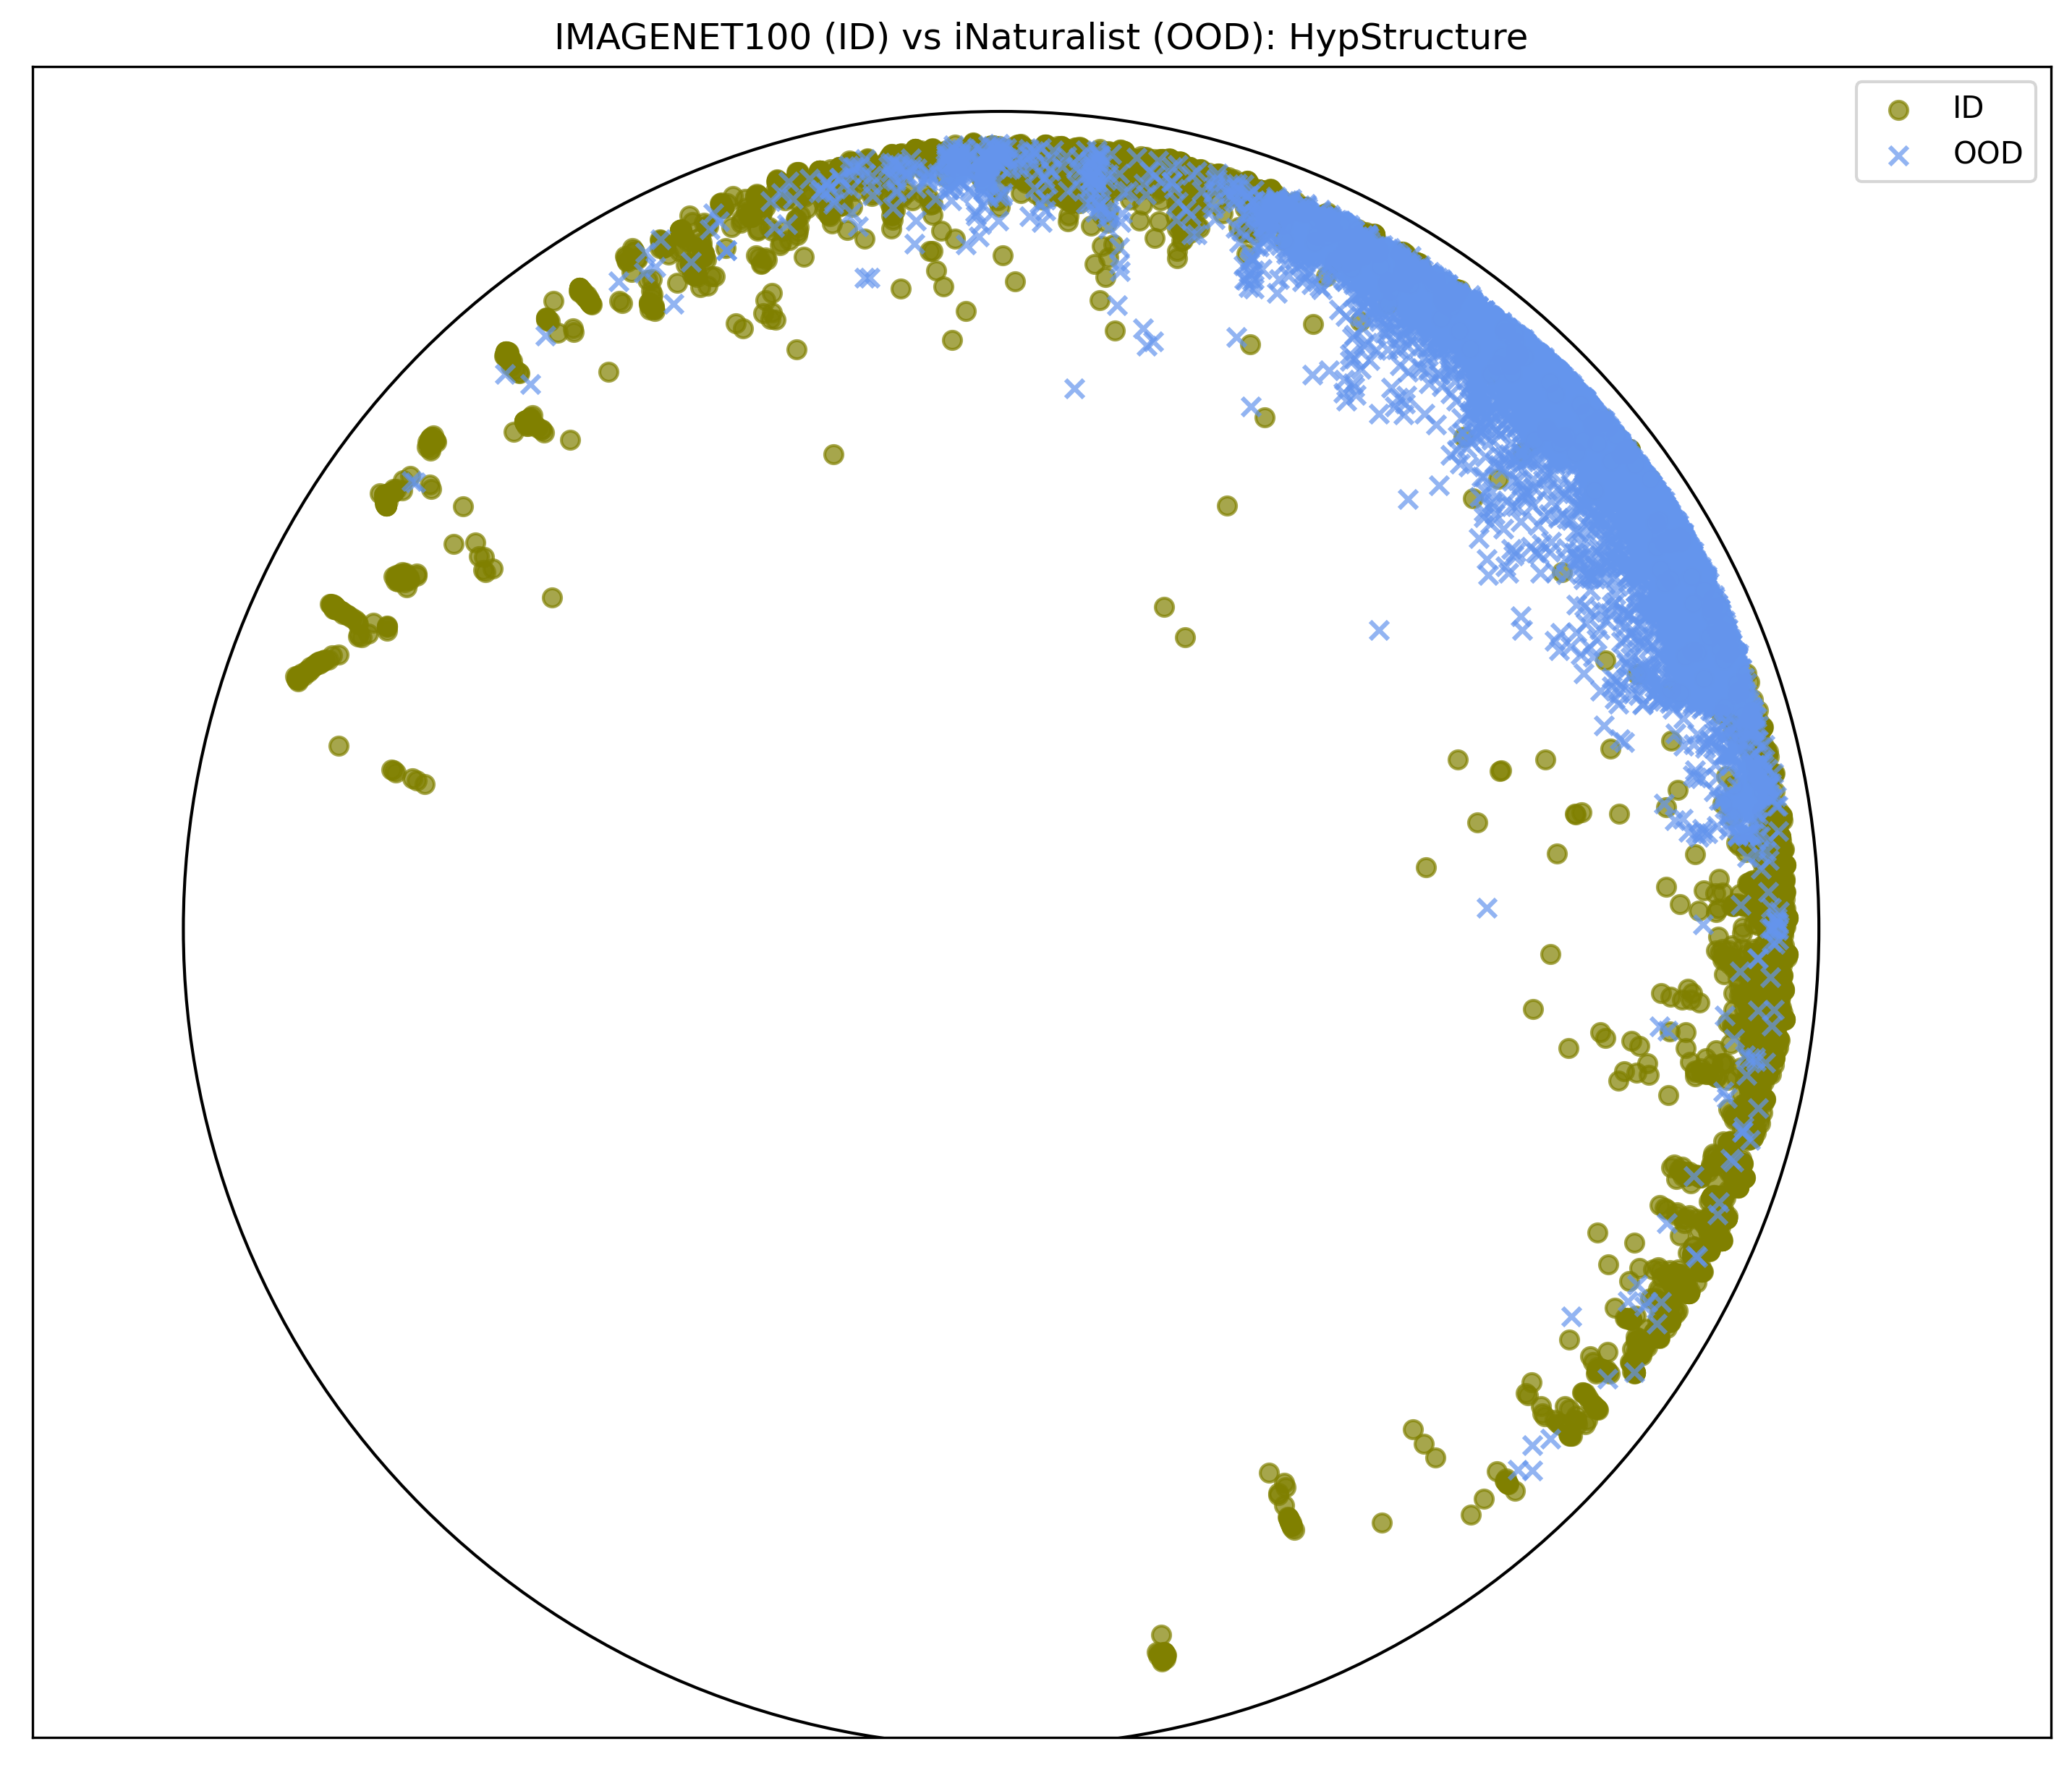
\includegraphics[width=.3\textwidth]{figures/hypstructure_im100_poincare_disk_ID_OOD.png}\\
{ (a)}&{ (b)} 
\end{tabular}
\caption{Hyperbolic UMAP Visualizations of ID-OOD separation on CIFAR10 and ImageNet100.}
\label{fig:add_viz_3}
\end{figure}

\subsection{Effect of Centering Loss and Embedding Internal Node}

Embedding the internal tree nodes in \texttt{HypStructure} $\mathcal{T}_{\text{int}}$ (as compared to only leaf nodes in prior work CPCC) and placing the root node at the center of the Poincaré disk with $\ell_{\text{center}}$ loss, helps in embedding the hierarchy more accurately. To understand the impact of these components, we first visualize the learnt representations from \texttt{HypStructure}, with and without these components - i.e. embedding internal nodes and a centering loss vs leaf only nodes, via UMAP in \Cref{fig:rebuttal_viz_3} (CIFAR100) and \Cref{fig:rebuttal_viz_2}  (ImageNet100). We also provide a performance comparison (fine accuracy) in \Cref{tab:hypstructure_comparison}.


\begin{table}[ht]
\centering
\resizebox{0.8\textwidth}{!}{
\begin{tabular}{lccc}
\toprule
\textbf{Method} & \textbf{CIFAR10} & \textbf{CIFAR100} & \textbf{ImageNet100} \\ \midrule
\texttt{HypStructure} (leaf only) & 94.54 & 76.22 & 89.85 \\
\texttt{HypStructure} (with internal nodes and centering) & \textbf{94.79} & \textbf{76.68} & \textbf{90.12} \\ \bottomrule
\end{tabular}
}
\vspace{0.4cm}
\caption{Fine accuracy comparison of \texttt{HypStructure} with vs. without internal nodes and centering on CIFAR10, CIFAR100, and ImageNet100 datasets.}
\label{tab:hypstructure_comparison}
\end{table}


First, based on Figures \Cref{fig:rebuttal_viz_3} and \Cref{fig:rebuttal_viz_2}, one can note that in the leaf-only setting without embedding internal nodes and centering loss (figures on the left), the samples belonging to the fine classes which share the same parent (same color) are in close proximity reflecting the hierarchy accurately, however the samples are not spread evenly. With the embedding of internal nodes and a centering loss (right), we note that the representations are spread between the center (root) to the boundary as well as across the Poincaré disk, which is more representative of the original hierarchy. This also leads to performance improvements as can be seen in \Cref{tab:hypstructure_comparison}. 

\begin{figure}[ht]
\centering
\begin{tabular}{cc}
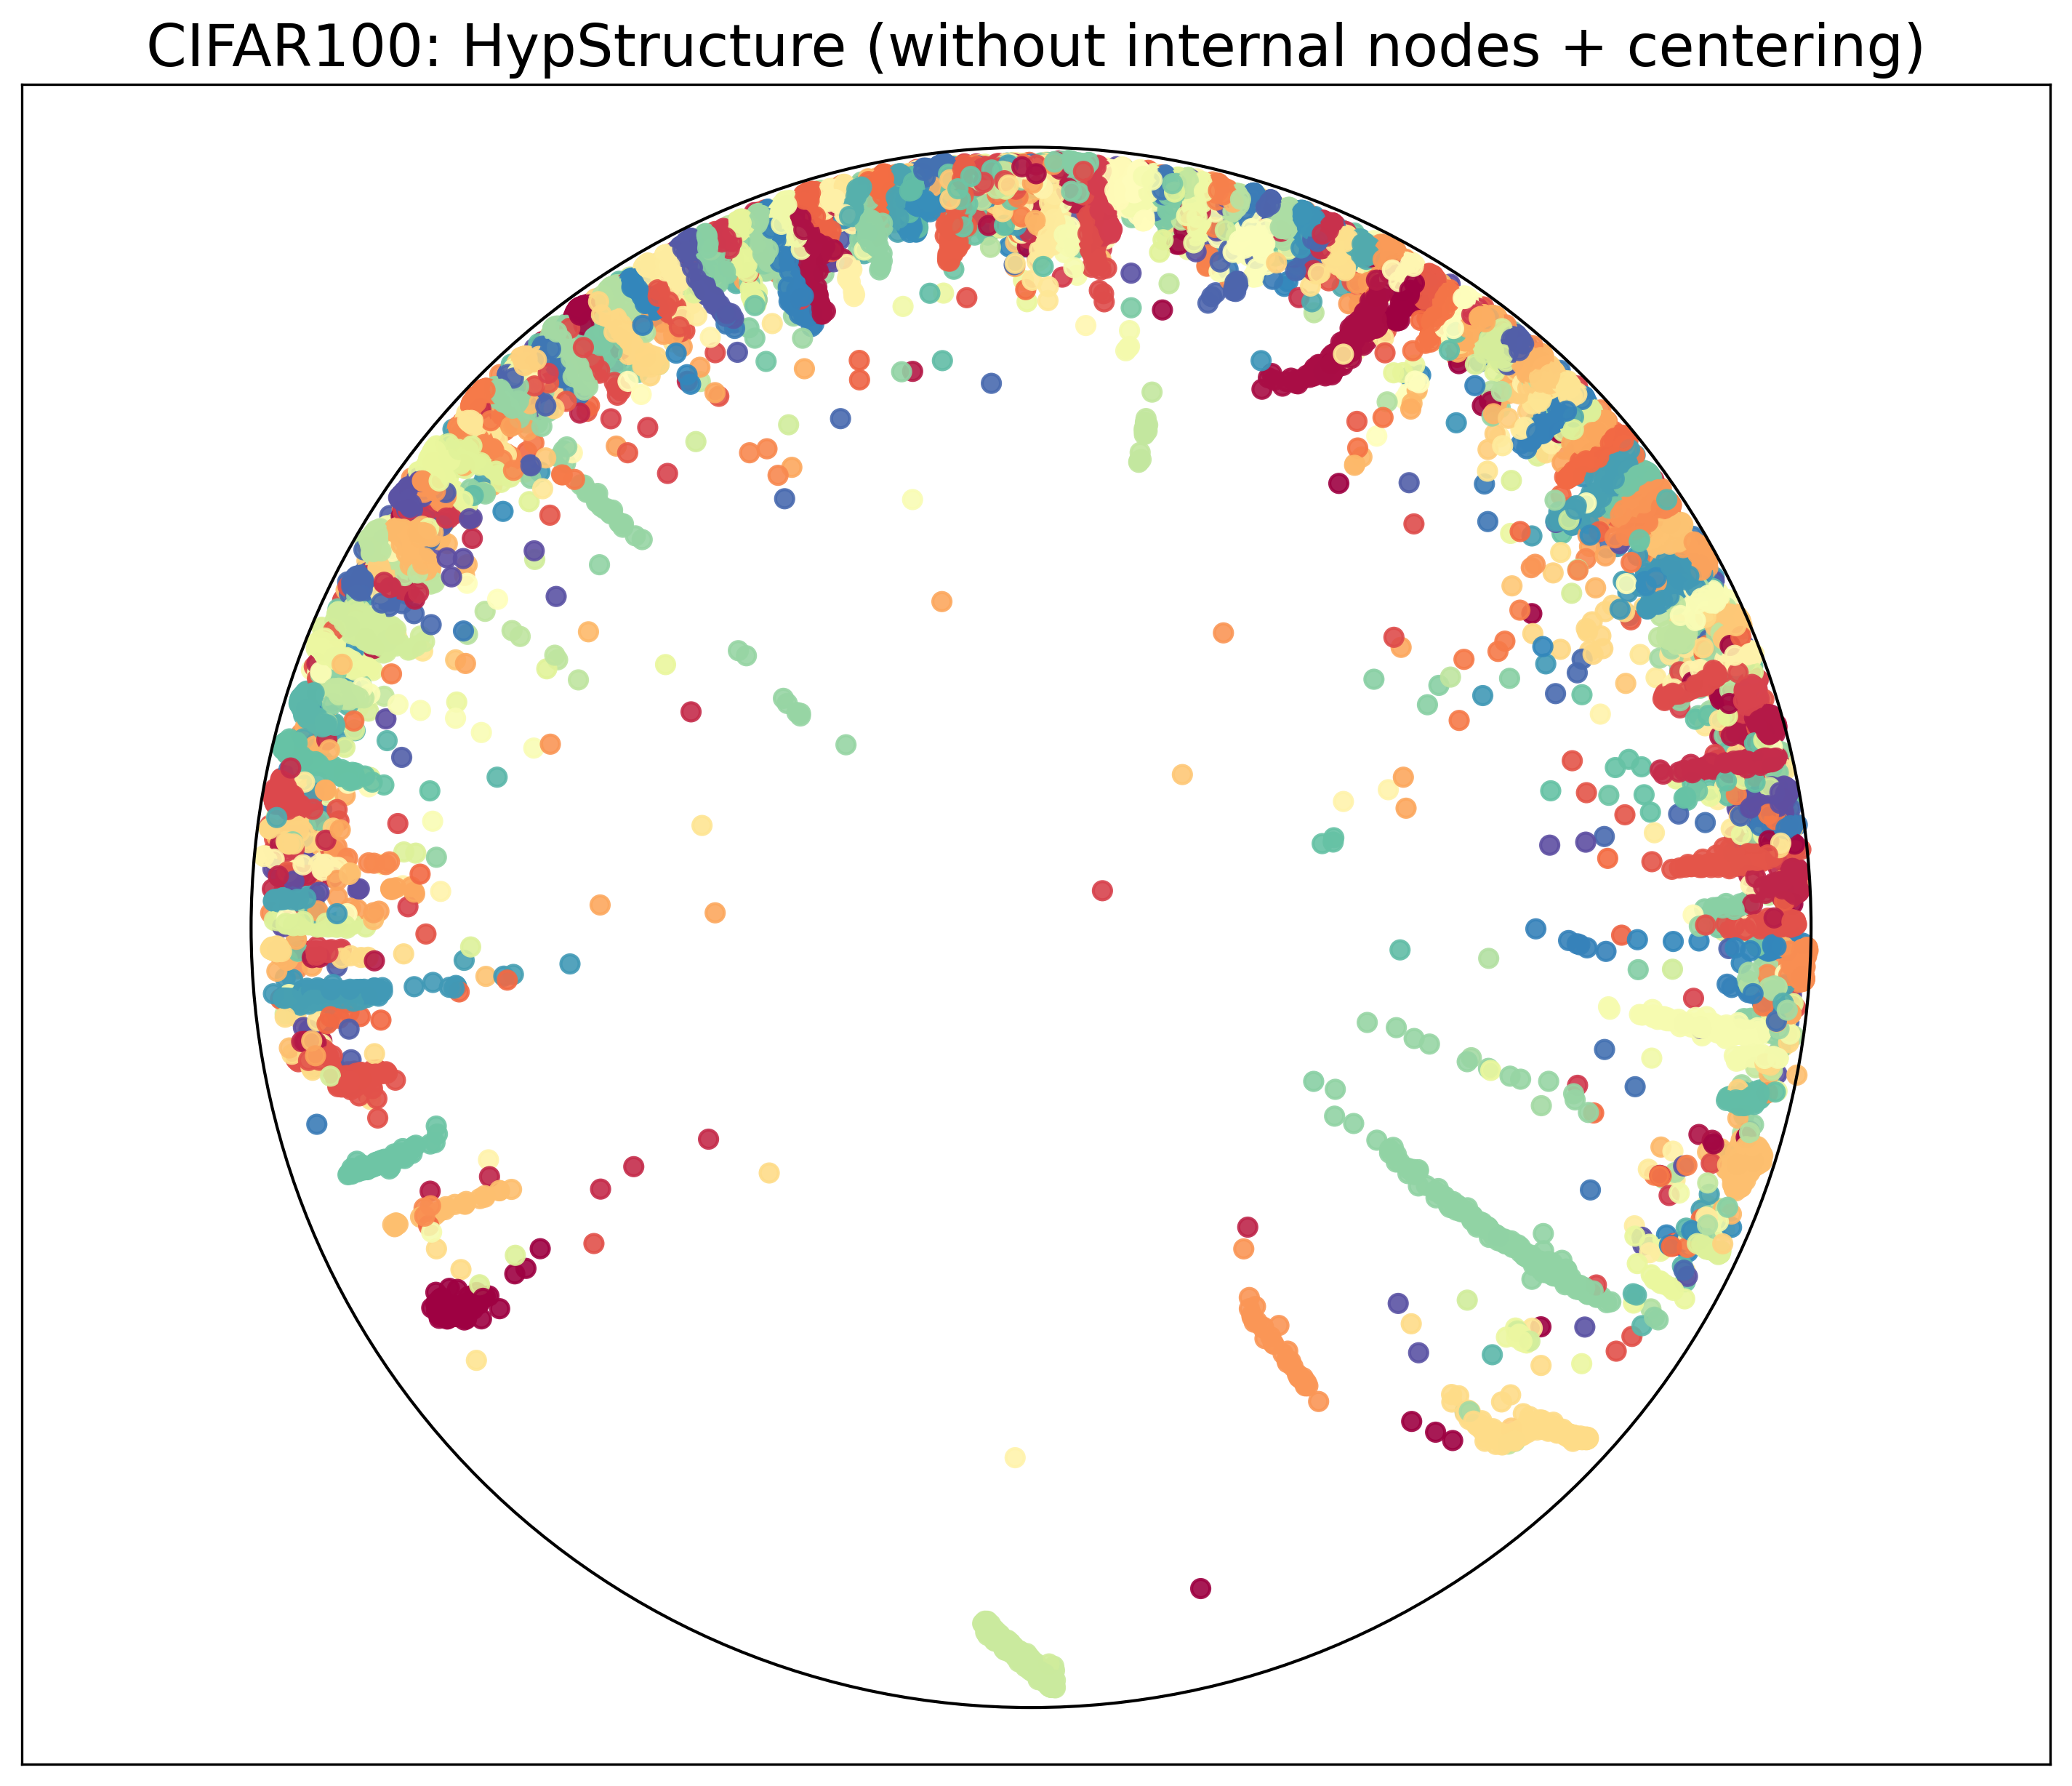
\includegraphics[width=.35\textwidth]{figures/hypstructure_poincare_disk_cifar100_without_internal_centering.png}&
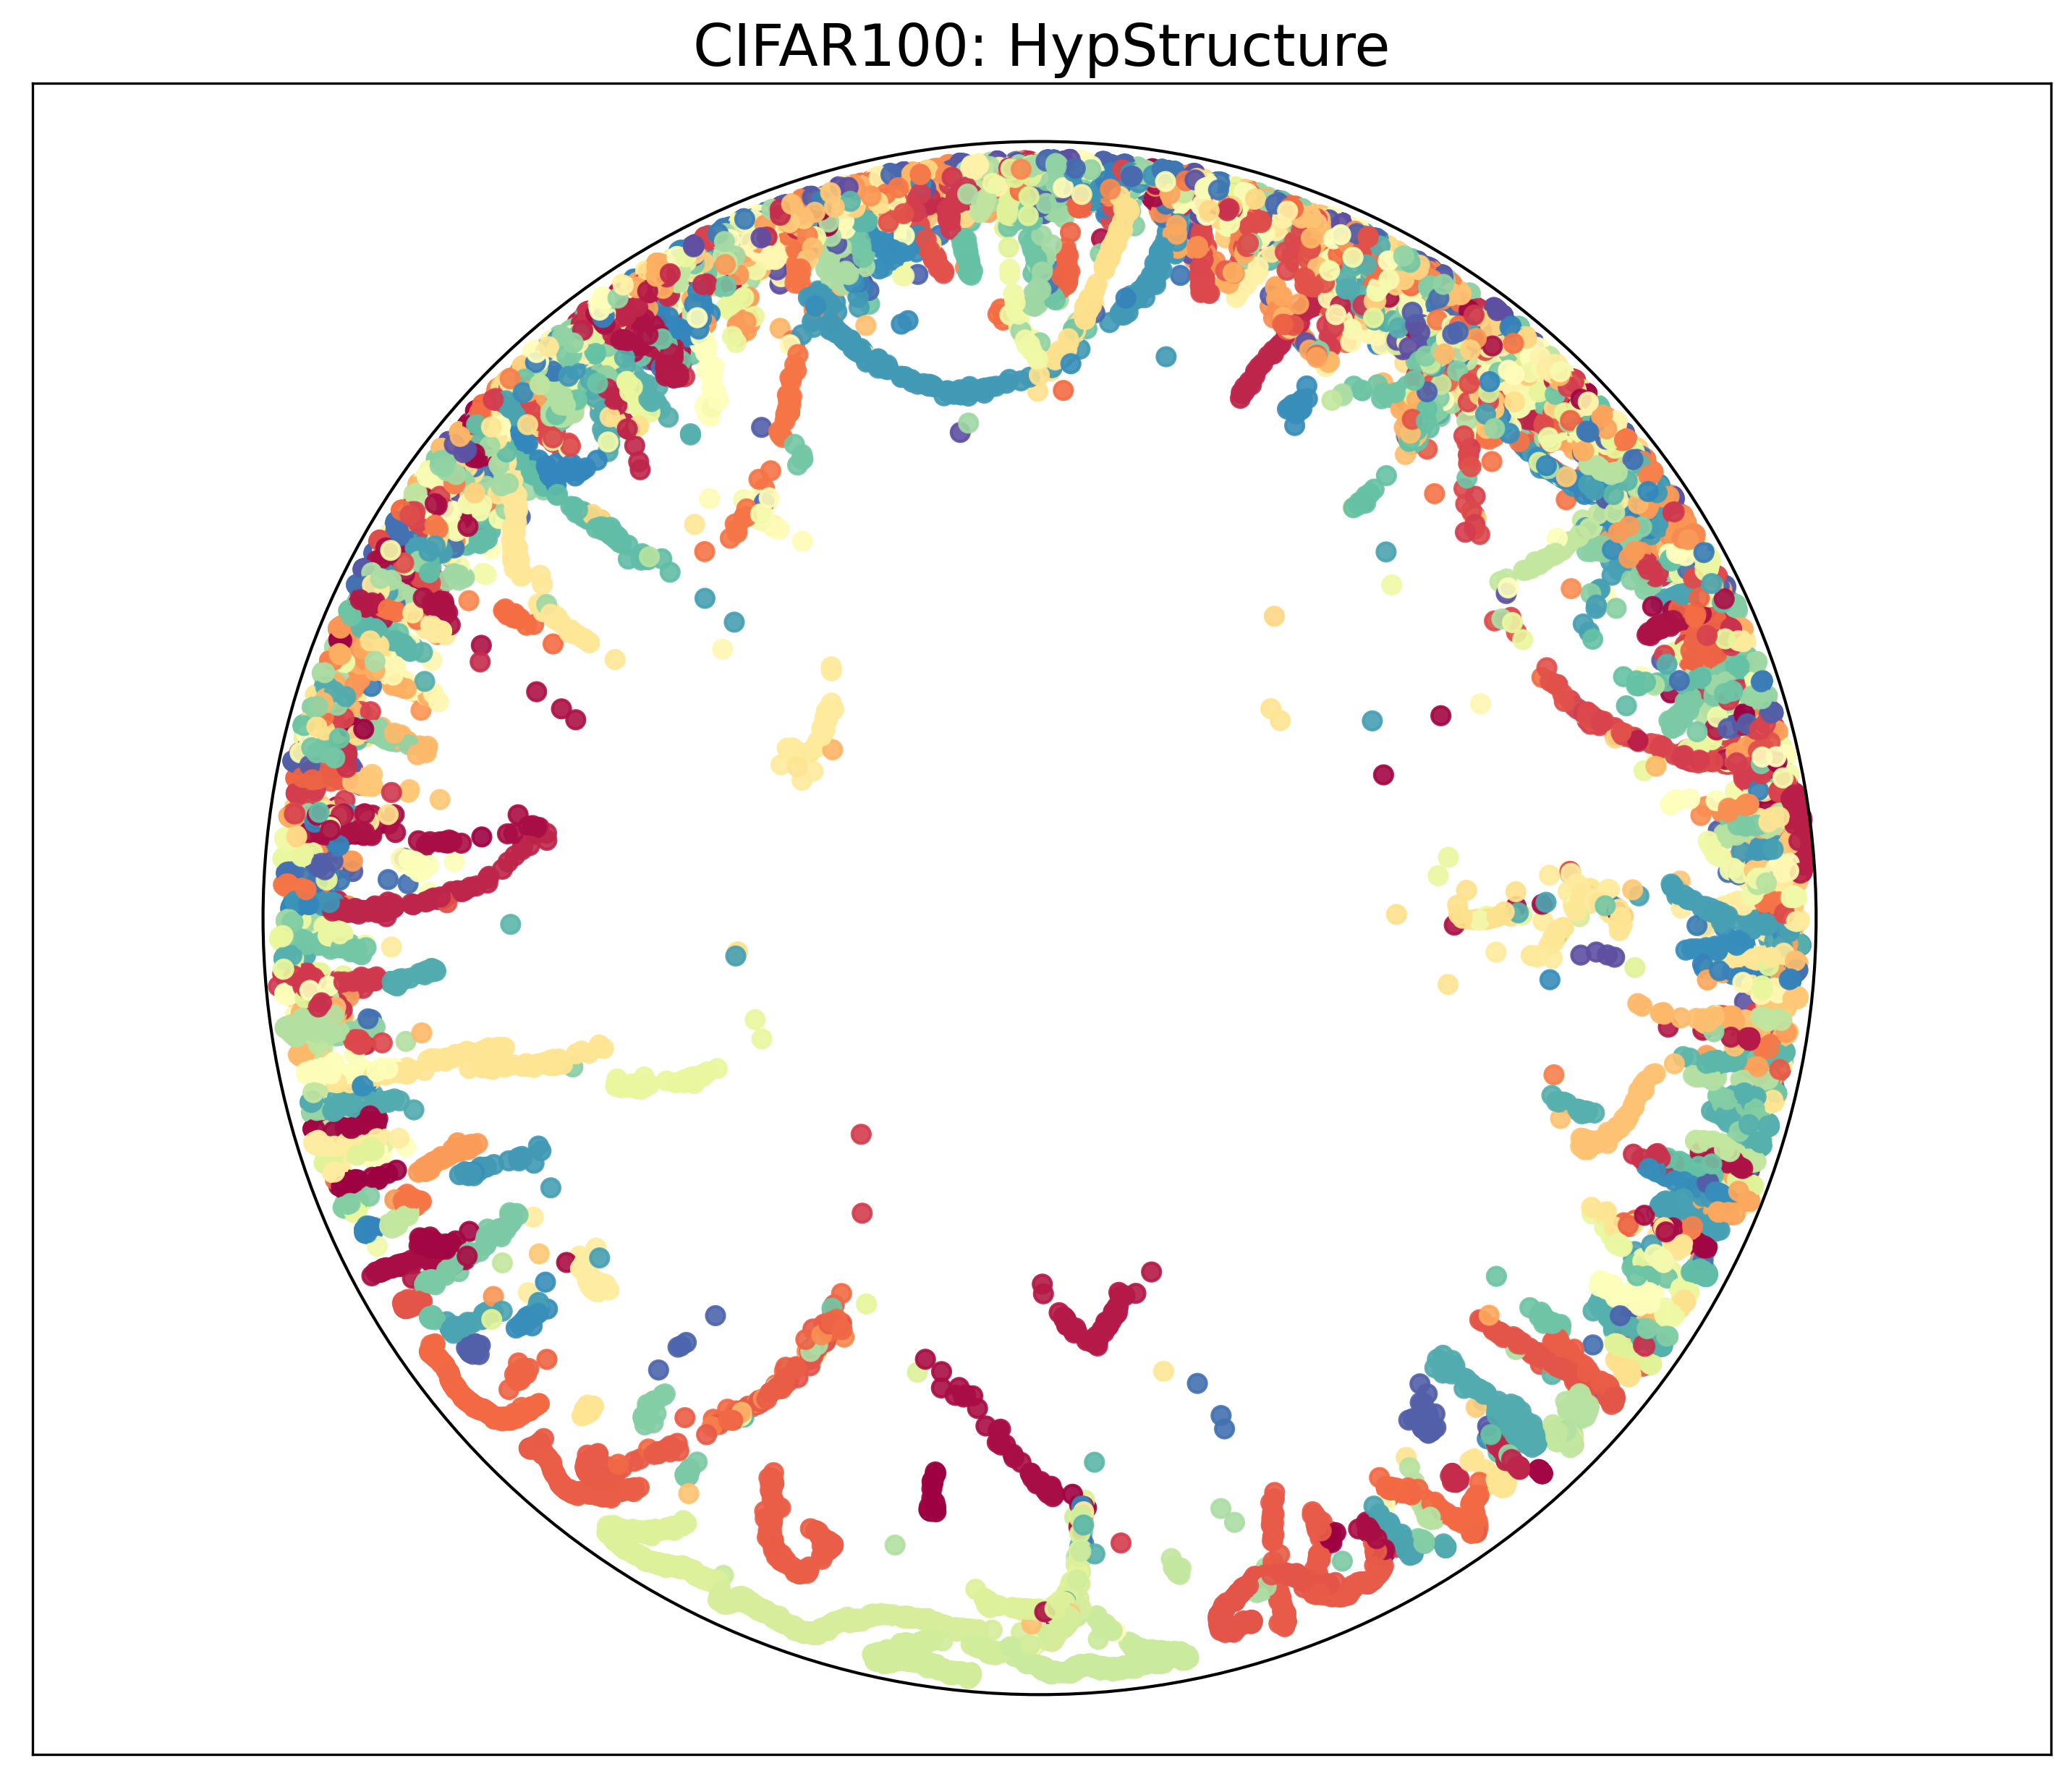
\includegraphics[width=.35\textwidth]{figures/hypstructure_poincare_disk_cifar100.png}\\
{ (a)}&{ (b)} 
\end{tabular}
\caption{Hyperbolic UMAP Visualizations on CIFAR100 using \texttt{HypStructure} without embedding the internal nodes and a hyperbolic centering loss (left), and with embedding the internal nodes along with a centering loss (right).}
\label{fig:rebuttal_viz_3}
\end{figure}


\begin{figure}[ht]
\centering
\begin{tabular}{cc}
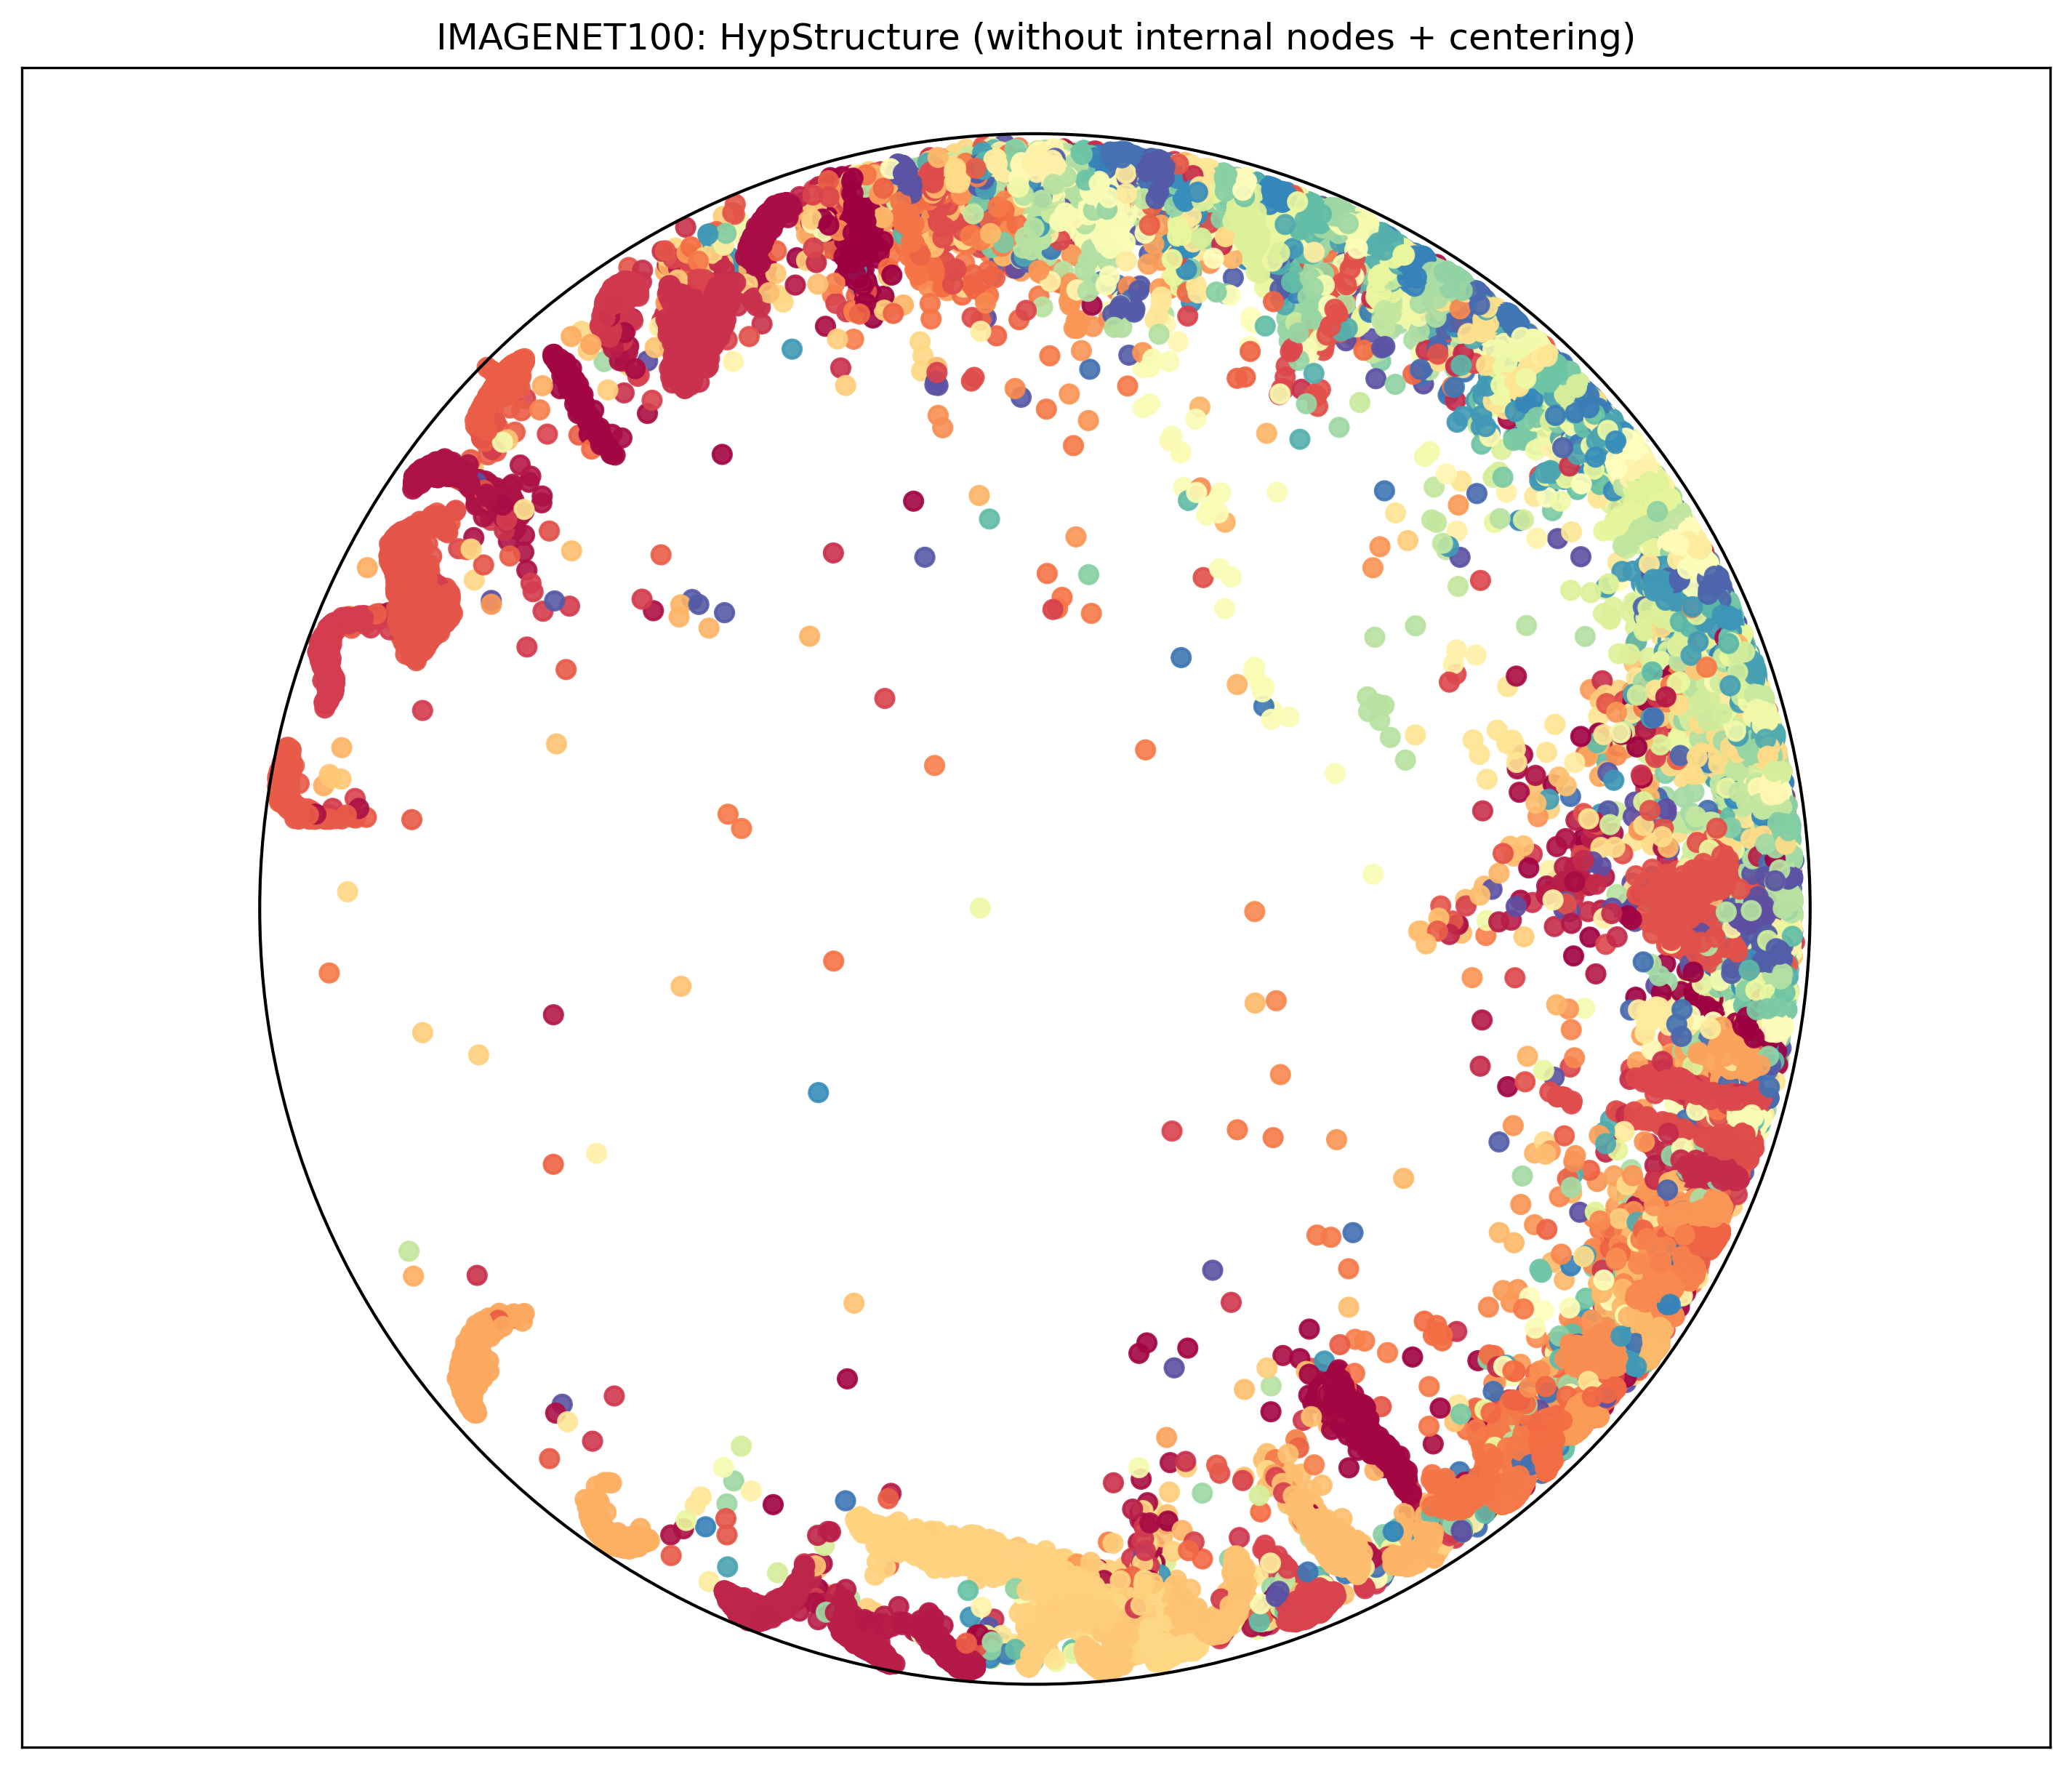
\includegraphics[width=.35\textwidth]{figures/hypstructure_poincare_disk_imagenet100_without_internal_centering.png}&
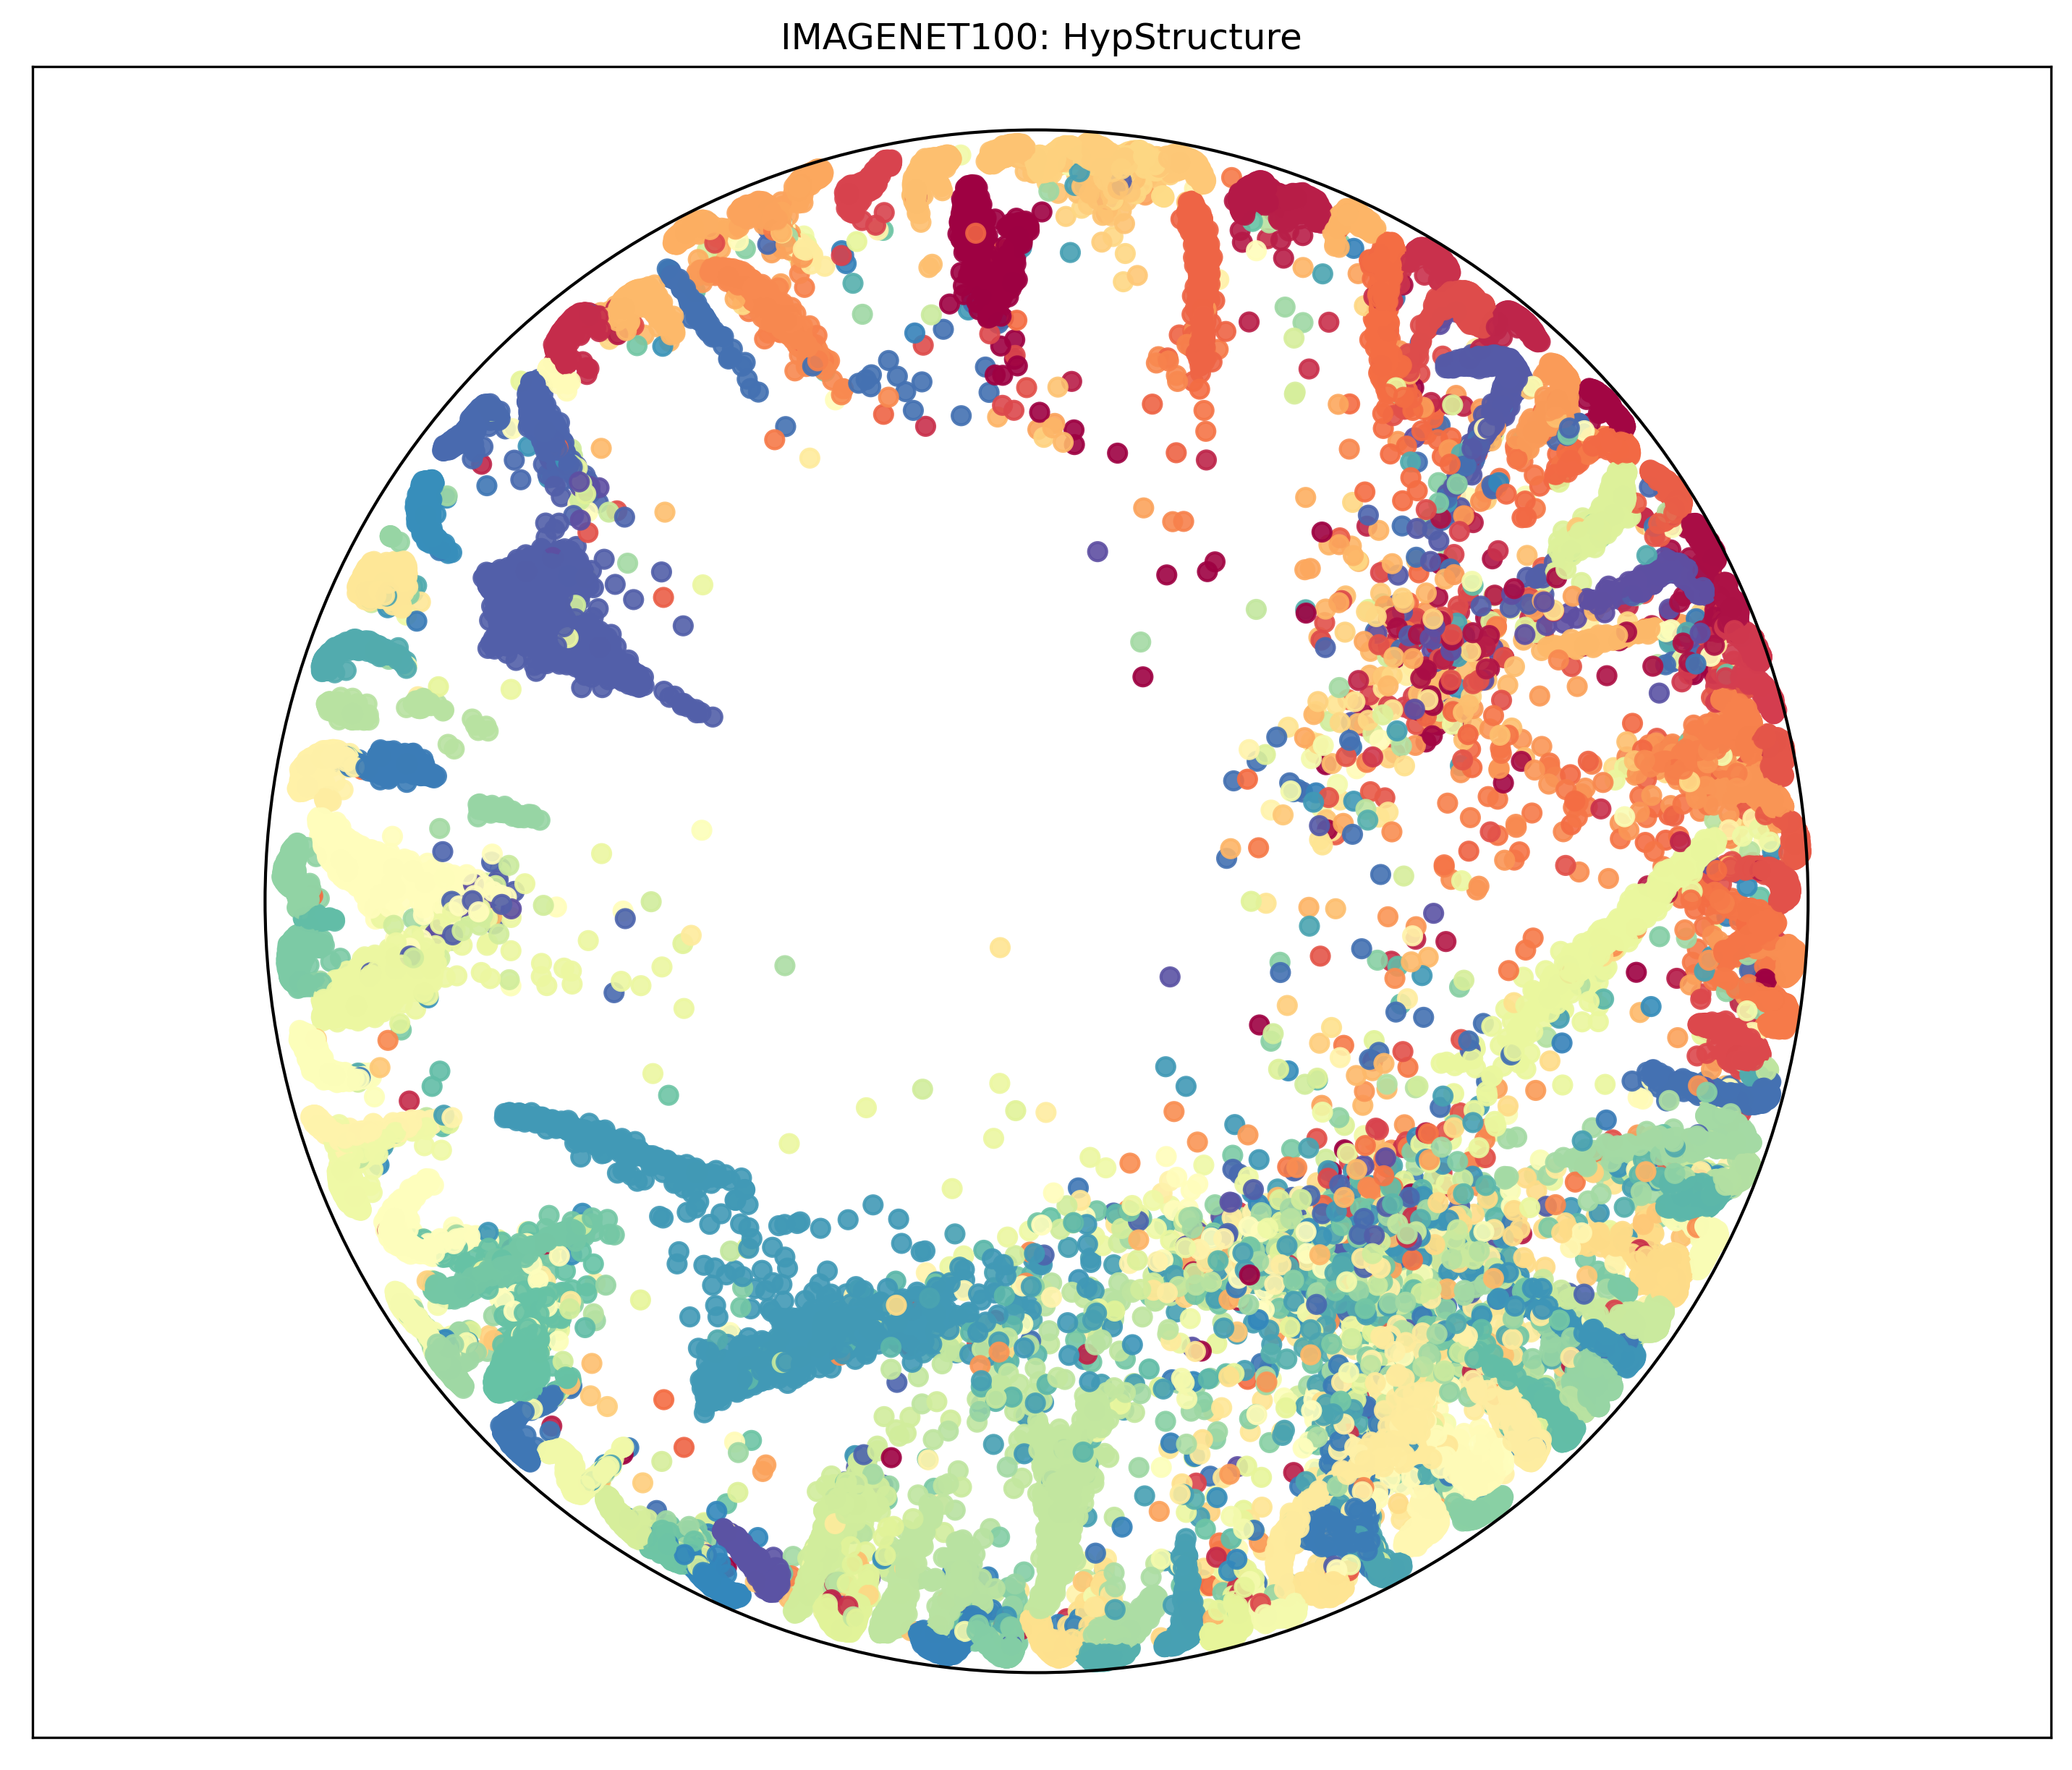
\includegraphics[width=.35\textwidth]{figures/hypstructure_poincare_disk_imagenet100.png}\\
{ (a)}&{ (b)} 
\end{tabular}
\caption{Hyperbolic UMAP Visualizations on ImageNet100 using \texttt{HypStructure} without embedding the internal nodes and a hyperbolic centering loss (left), and with embedding the internal nodes along with a centering loss (right).}
\label{fig:rebuttal_viz_2}
\end{figure}


\subsection{Effect of Label Hierarchy Weights}
Compared to ranking-based hyperbolic losses \citep{nickel2017poincare}, our HypCPCC factors in absolute values of the node-to-node distances. The learned hierarchy with HypCPCC will not only implicitly encode the correct parent-child relations, but can also learn more complex and weighted hierarchical relationships more accurately.
To demonstrate this, we modify the CIFAR10 tree hierarchy, and gradually increase the weight for the left transportation branch to 2$\times$ and 4$\times$ and use new weighted trees for the CPCC tree distance computation. We visualize the learnt representations in \Cref{fig:rebuttal_viz_4} and we can observe that in the learned representations from left to right, the distance between the transportation classes (blue) are larger as compared to other classes, as expected.

\begin{figure}[ht]
\centering
\begin{tabular}{ccc}
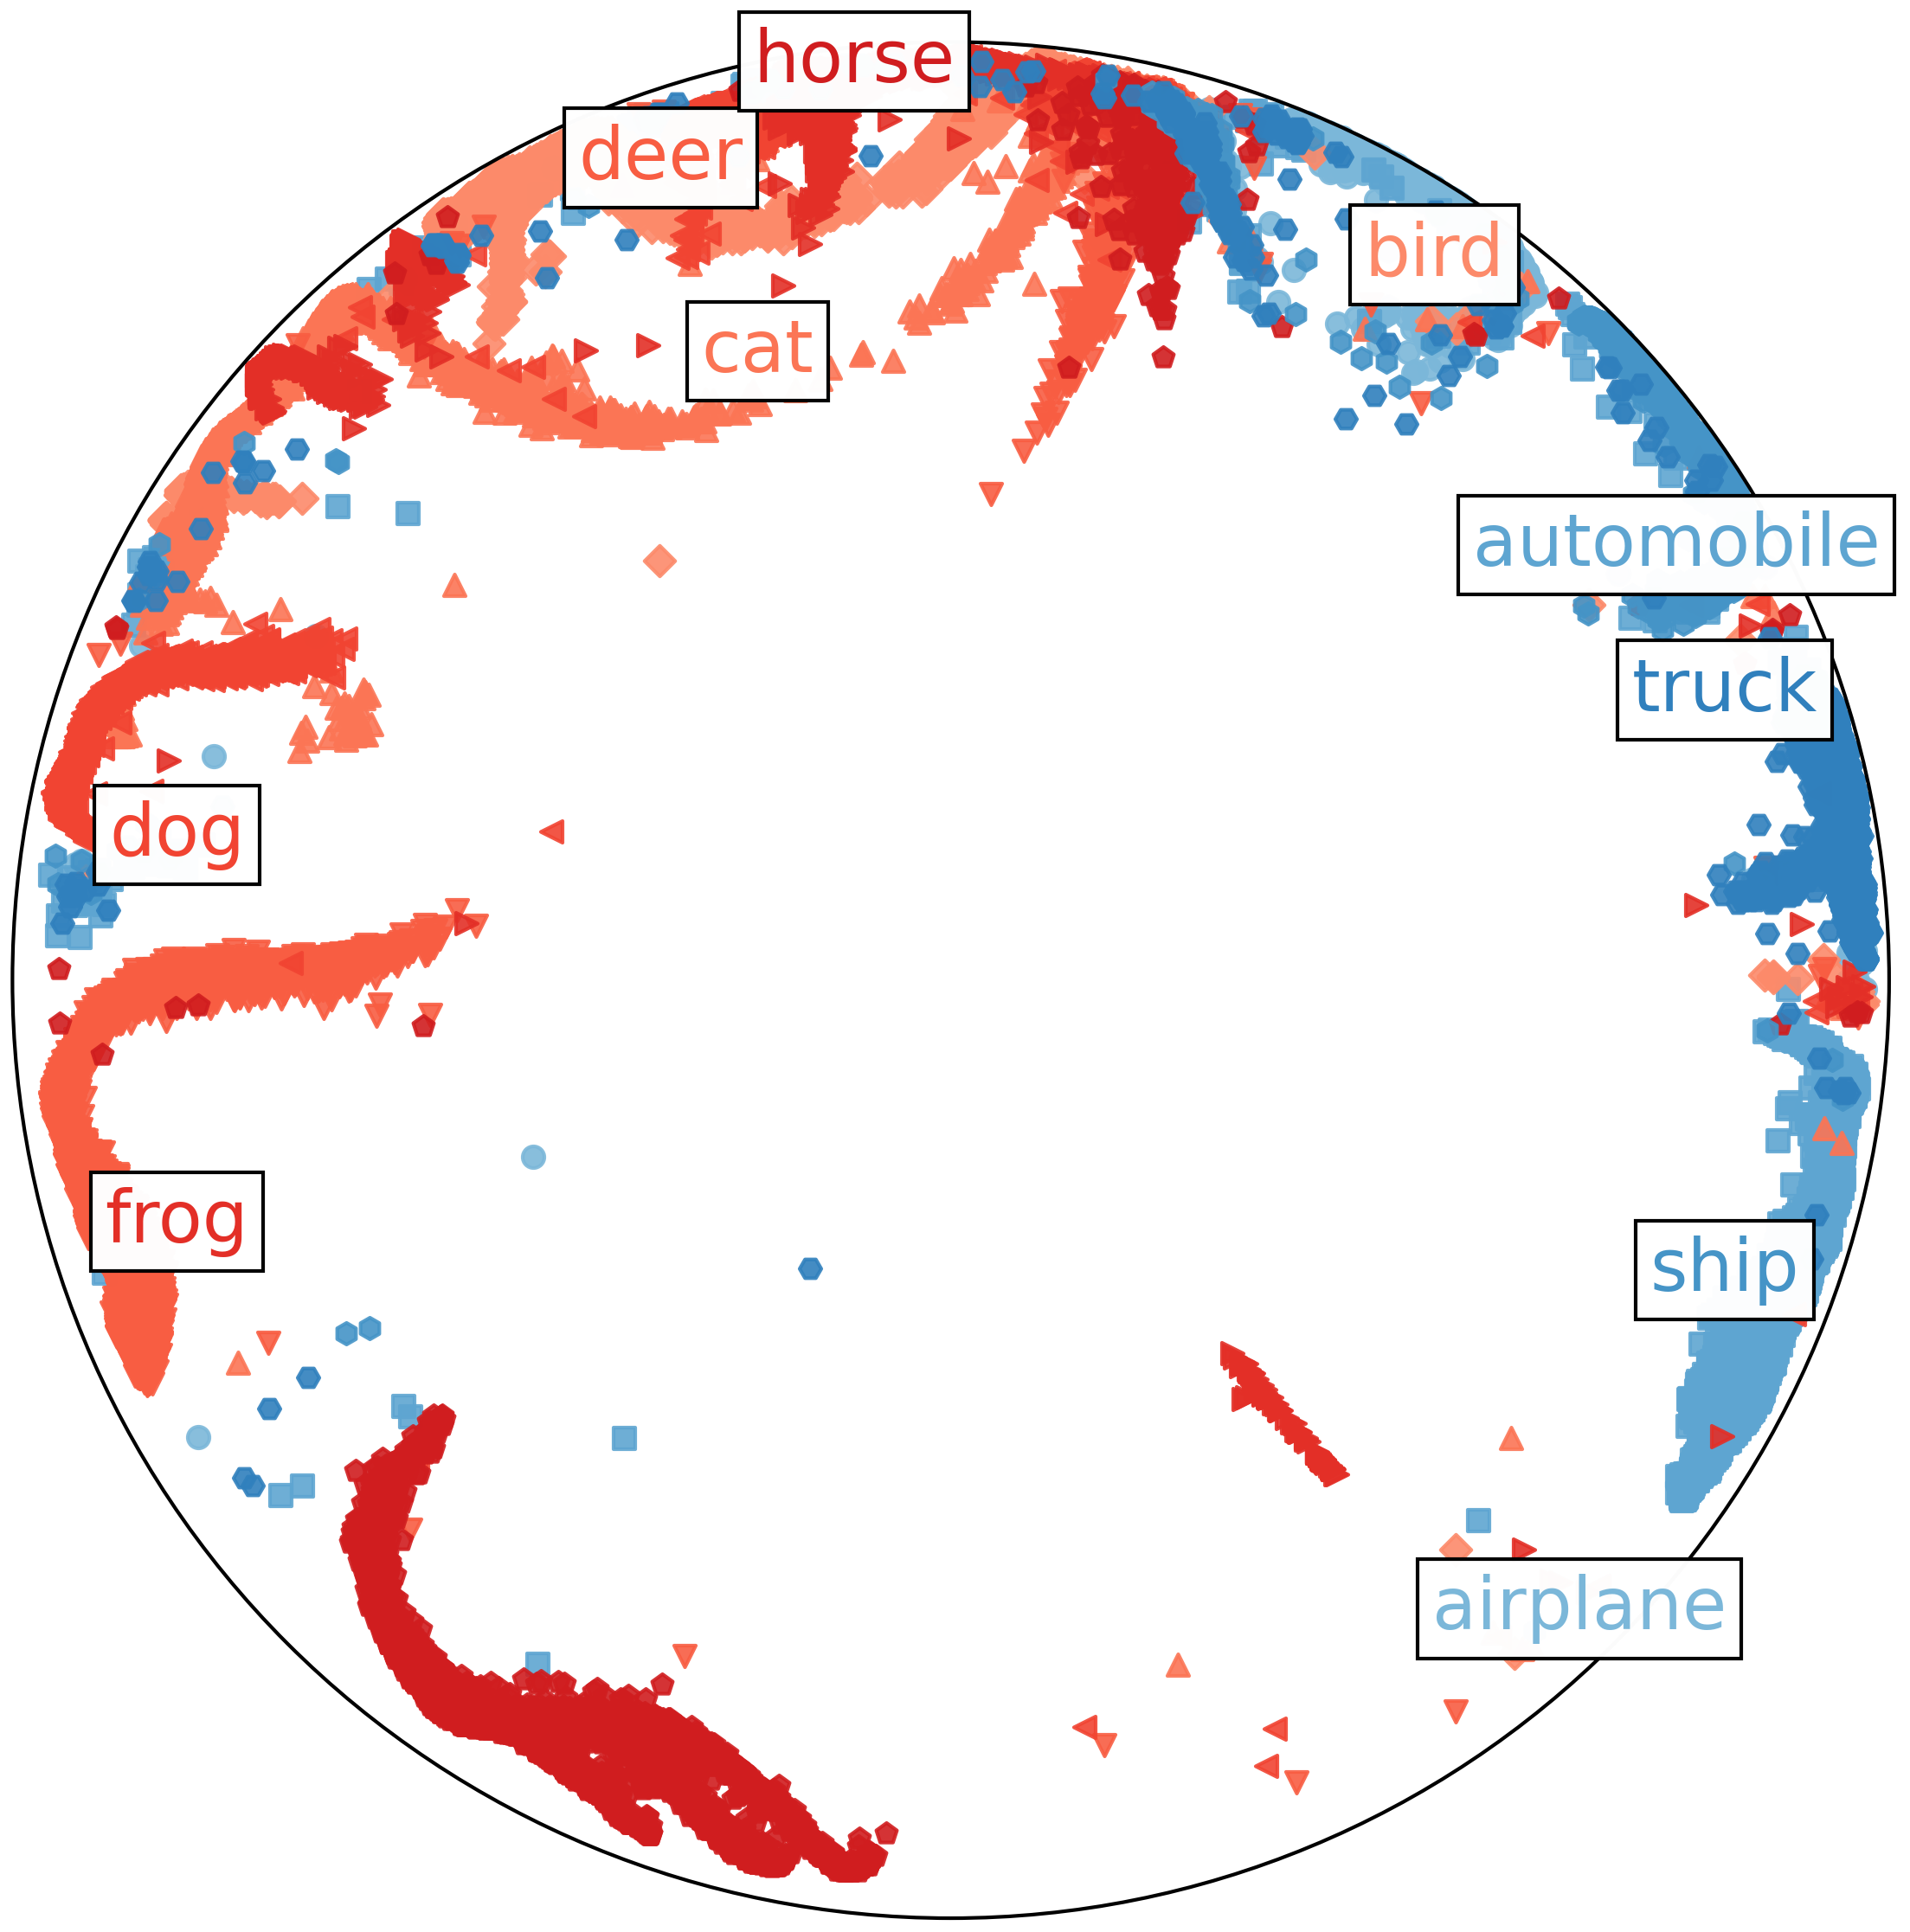
\includegraphics[width=.19\textwidth]{figures/hypstructure_cifar10_centers_main_1.png}&
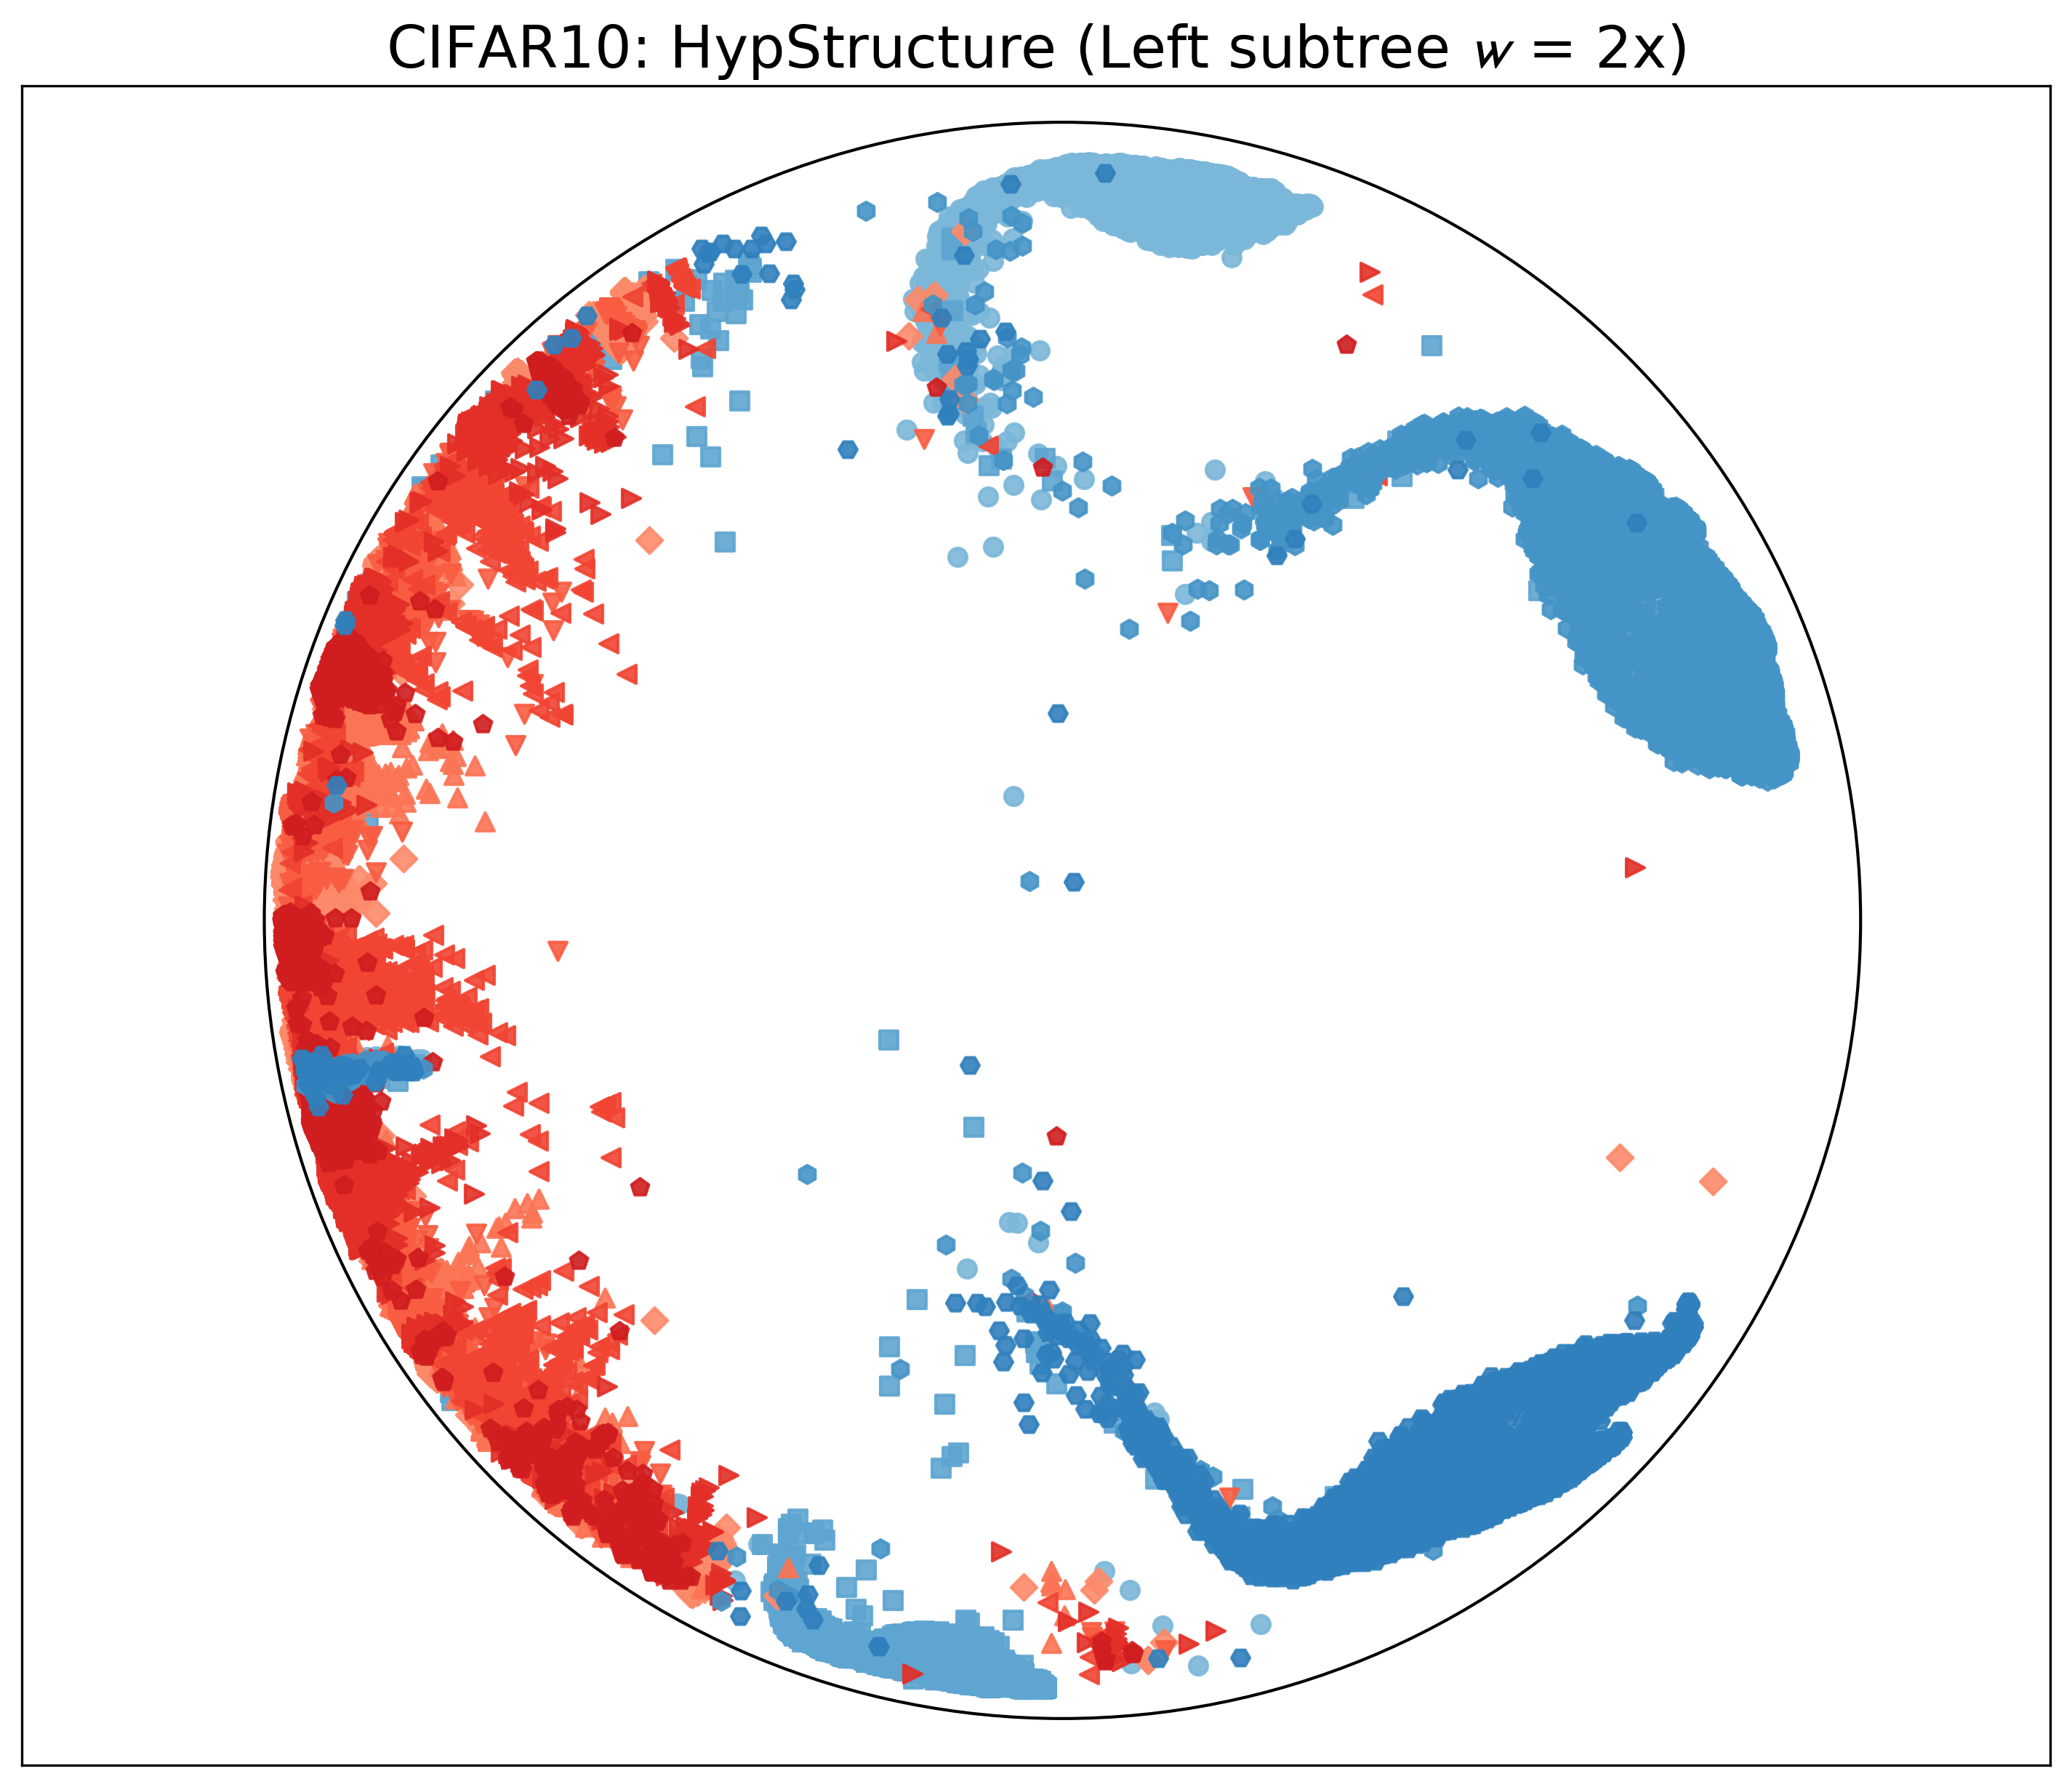
\includegraphics[width=.25\textwidth]{figures/hypstructure_poincare_disk_cifar10_weights2x.png} & 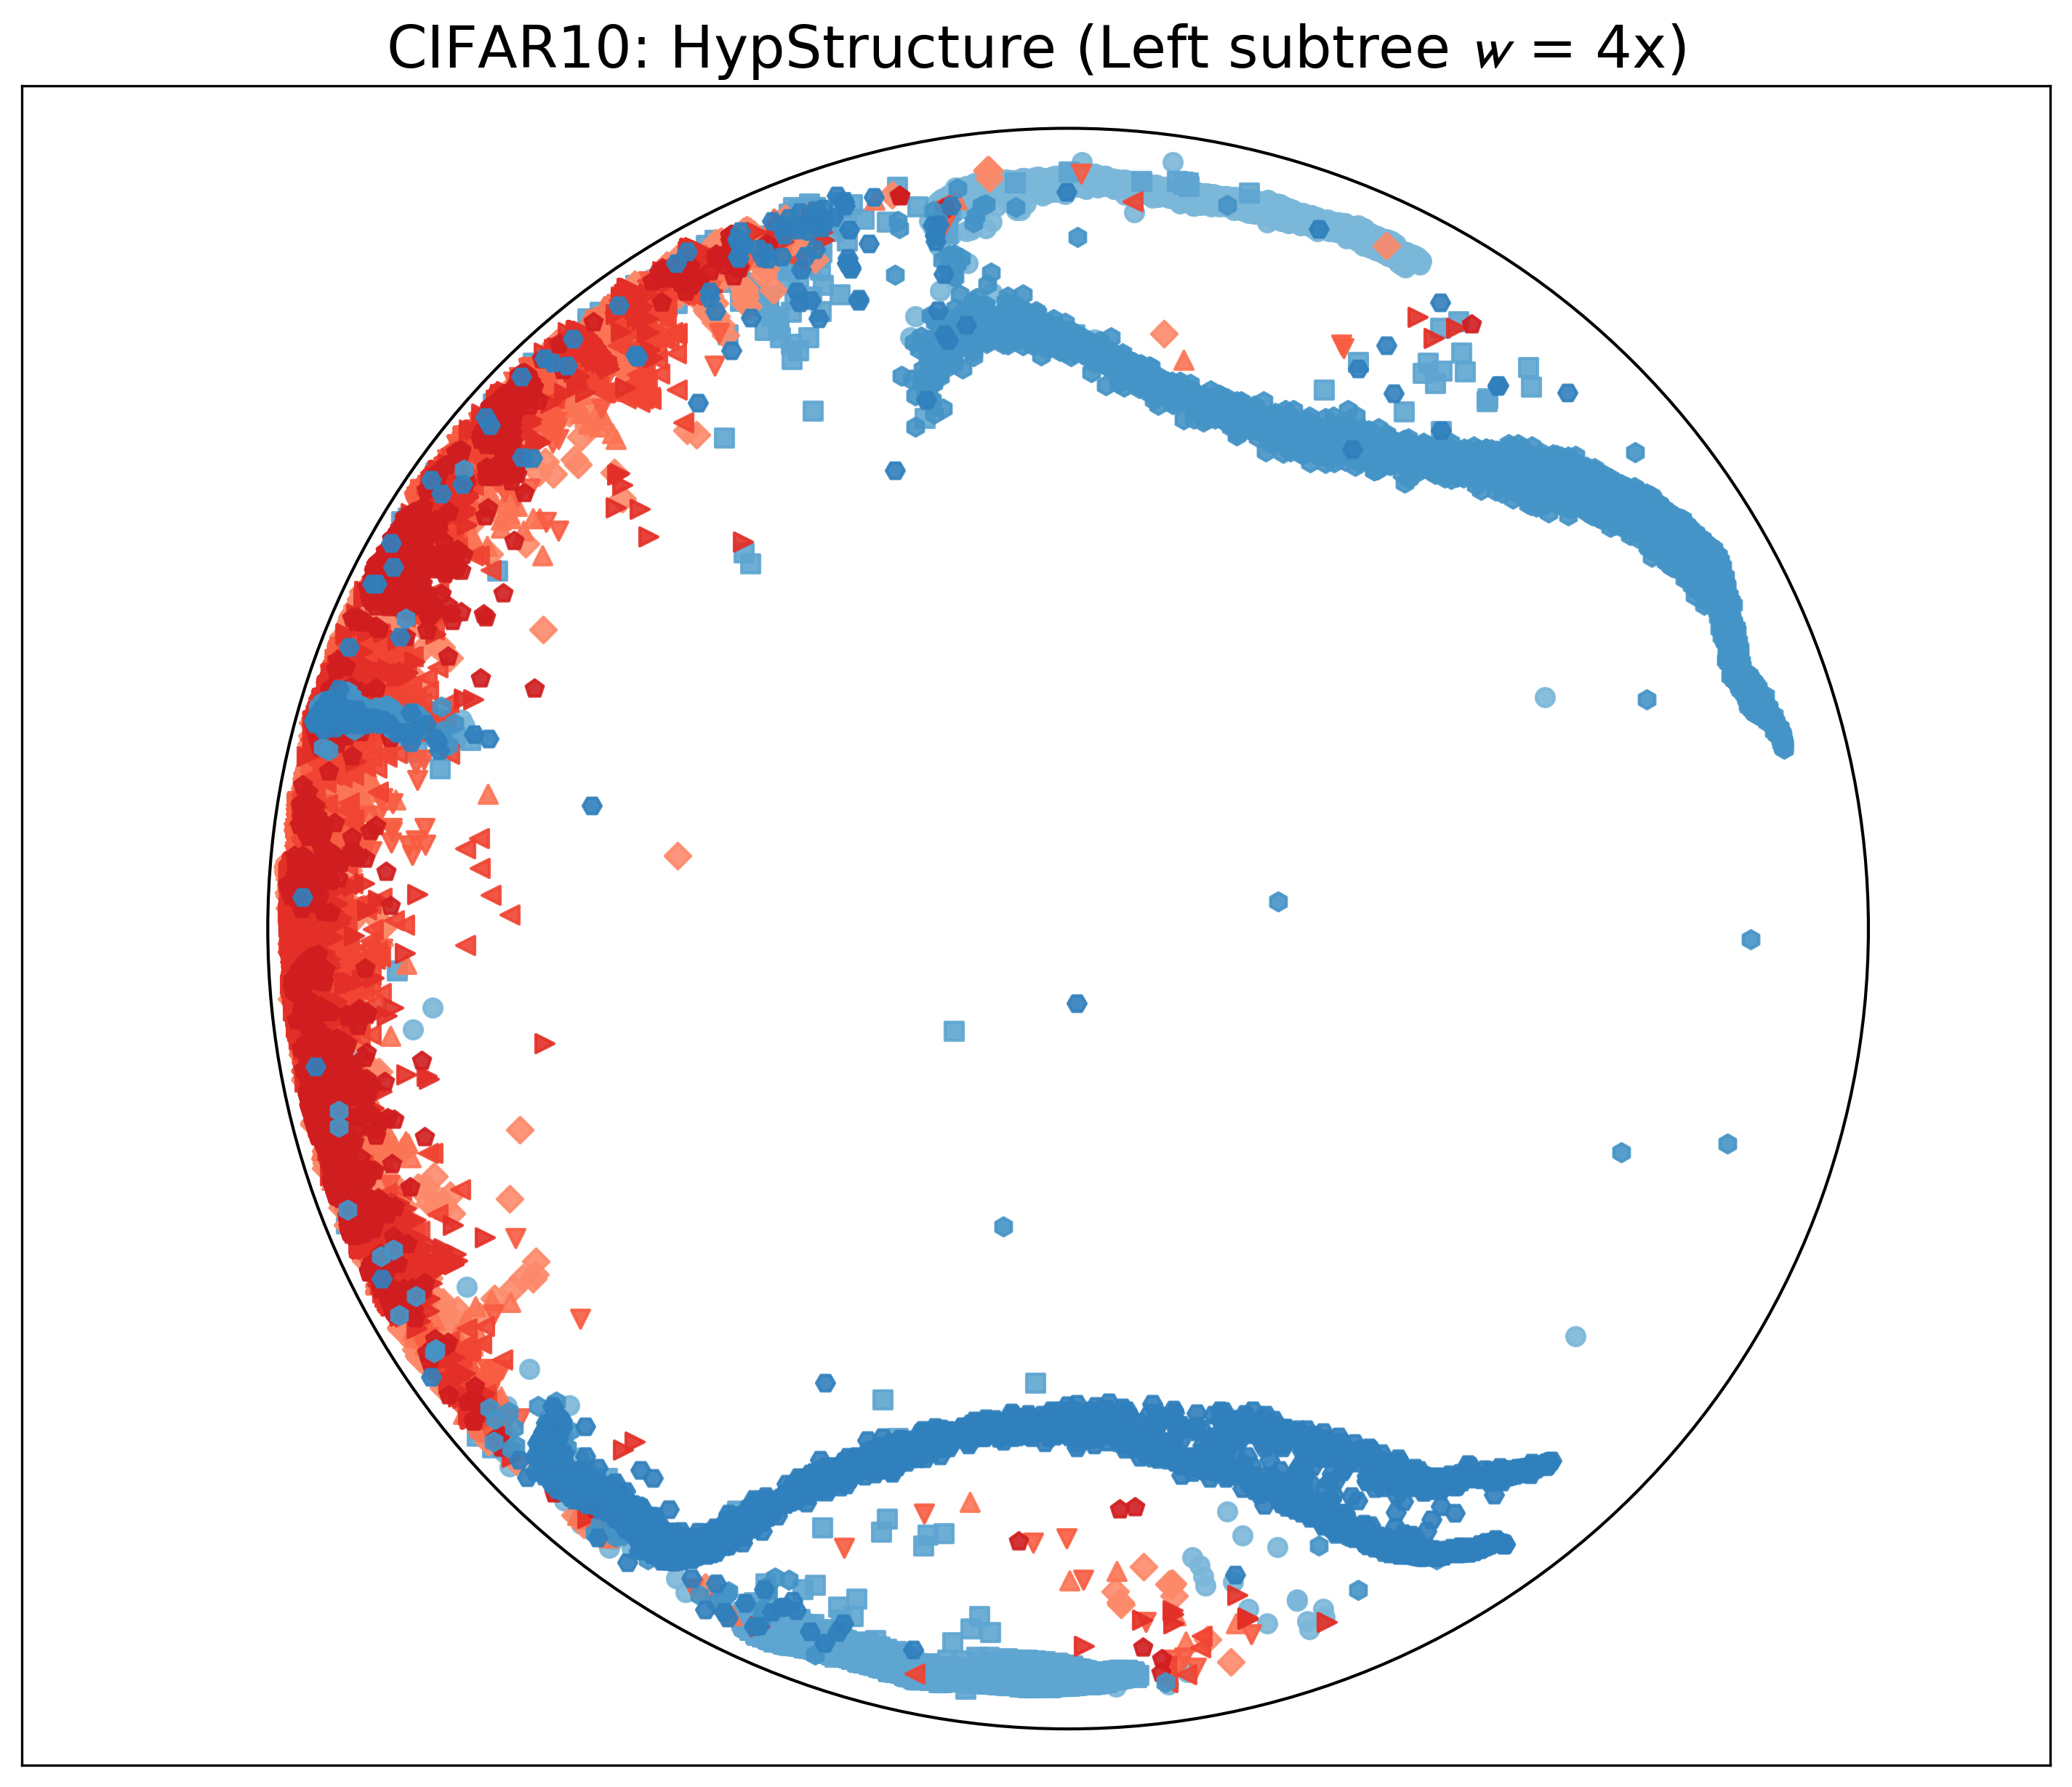
\includegraphics[width=.25\textwidth]{figures/hypstructure_poincare_disk_cifar10_weights4x.png}\\
{ (a)}&{ (b) } & {(c)} 
\end{tabular}
\caption{HypStructure can learn more nuanced representations with weighted hierarchy trees. Hyperbolic UMAP visualizations on CIFAR10 using HypStructure with differently weighted left-subtrees.}
\label{fig:rebuttal_viz_4}
\end{figure}

\subsection{Effect of Klein Averaging}
We experiment with the two HypCPCC variants, using Klein Averaging or Euclidean mean for centroid computation, as mentioned in \Cref{sec:hypstructure-method} and report the results in \Cref{tab:euc_vs_klein}. We empirically observe that using the Klein averaging leads to performance improvements across datasets. 

\begin{table}[ht]
\centering
\resizebox{0.5\textwidth}{!}{
\begin{tabular}{lccc}
\toprule
\textbf{Method} & \textbf{CIFAR10} & \textbf{CIFAR100} & \textbf{ImageNet100} \\ \midrule
Euclidean & 94.56 & 75.64 & 90.08 \\
Klein & \textbf{94.79} & \textbf{76.68} & \textbf{90.12} \\ \bottomrule
\end{tabular}
}
\vspace{0.4cm}
\caption{Fine accuracy comparison between Euclidean and Klein centroid computation methods in HypCPCC on CIFAR10, CIFAR100, and ImageNet100 datasets.}
\label{tab:euc_vs_klein}
\end{table}



\subsection{Experiments with the Hyperbolic Supervised Contrastive Loss}
\label{app:sec_hypsupcon}

We experiment with the Hyperbolic Supervised Contrastive Loss as proposed in \citep{ge2022hyperbolic} 
as the choice of the $\ell_\text{Flat}$ loss and refer to this loss as $\ell_\text{HypSupCon}$. We follow the original setup as described by the authors for the measurement of the $\ell_\text{HypSupCon}$, where the 
representations from the encoders are not normalized directly, instead an exponential map is used to project these features from the Euclidean space to the Poincaré ball first. Then, the inner product measurement in the $\ell_\text{SupCon}$ is replaced with the negative hyperbolic distances in the Poincaré ball to compute the $\ell_\text{HypSupCon}$ loss. We also experiment with our proposed methodology \texttt{HypStructure} along with the $\ell_\text{HypSupCon}$ loss and report the classification accuracies and hierarchy embedding metrics for both these settings in Table \ref{tab:hypsupcon_evals}. We further report the OOD detection performance on CIFAR10, CIFAR100 and ImageNet100 as in-distribution datasets for both of these settings in Tables \ref{tab:hypsupcon_c10_ood}, \ref{tab:hypsupcon_c100_ood} and \ref{tab:hypsupcon_im10_ood} respectively. We observe that using \texttt{HypStructure} with a hyperbolic loss such as $\ell_\text{HypSupCon}$ as the Flat loss leads to improvements in accuracy across classification and OOD detection tasks while also improving the quality of embedding the hierarchy. This demonstrates the wide applicability of our proposed method \texttt{HypStructure} which can be used in conjunction with both euclidean and non-euclidean classification losses. 


\begin{table}[ht]
\caption{Evaluation of hierarchical information distortion and classification accuracy using \texttt{HypSupCon} \citep{ge2022hyperbolic} as $\ell_\text{Flat}$. All metrics are reported as mean (standard deviation) over 3 seeds.}
  \vspace{0.2cm}
  \centering
        \resizebox{0.8\textwidth}{!}{
            \begin{tabular}{lcccccccc}
                \toprule
                \multirow{2}{*}{\textbf{\begin{tabular}[c]{@{}c@{}}Dataset\\ (Backbone)\end{tabular}}} & \multirow{2}{*}{\textbf{Method}} & \multicolumn{2}{c}{\textbf{Distortion of Hierarchy}} & \multicolumn{2}{c}{\textbf{Classification Accuracy}} \\
                \cmidrule(lr){3-4} \cmidrule(lr){5-6}
                & & \textbf{$\delta_{rel}$ ($\downarrow$)} & \textbf{CPCC ($\uparrow$)} & \textbf{Fine ($\uparrow$)} & \textbf{Coarse ($\uparrow$)} \\
                \midrule
                \multirow{2}{*}{\begin{tabular}[c]{@{}c@{}}CIFAR10\\ (ResNet-18)\end{tabular}} & Flat & 0.128 (0.007) &	0.745 (0.017) &	94.58 (0.04) &	98.96 (0.01) \\
                & \cellcolor{gray!20}\texttt{HypStructure}  & \cellcolor{gray!20}\textbf{0.017 (0.001)	} & \cellcolor{gray!20}\textbf{0.989 (0.001)} & \cellcolor{gray!20}\textbf{95.04 (0.02)} & \cellcolor{gray!20}\textbf{99.36 (0.02)} \\
                \midrule
                \multirow{2}{*}{\begin{tabular}[c]{@{}c@{}}CIFAR100\\ (ResNet-34)\end{tabular}} & Flat & 0.168 (0.002) &	0.664 (0.012) &	75.81 (0.06) &	85.26 (0.07) \\
                & \cellcolor{gray!20}\texttt{HypStructure} & \cellcolor{gray!20}\textbf{0.112 (0.005)} & \cellcolor{gray!20}\textbf{0.773 (0.008)	} & \cellcolor{gray!20}\textbf{76.22 (0.14)} & \cellcolor{gray!20}\textbf{85.83 (0.06)} \\
                \midrule
                \multirow{2}{*}{\begin{tabular}[c]{@{}c@{}}ImageNet100\\ (ResNet-34)\end{tabular}} & Flat & 0.157 (0.004) &	0.473 (0.004) &	89.87 (0.01) & 90.41 (0.01) \\
                & \cellcolor{gray!20}\texttt{HypStructure}  & \cellcolor{gray!20}\textbf{0.126 (0.002)	} & \cellcolor{gray!20}\textbf{0.714 (0.003)	} & \cellcolor{gray!20}\textbf{90.26 (0.01)} & \cellcolor{gray!20}\textbf{90.95 (0.01)} \\
                \bottomrule
            \end{tabular}
                }
    \label{tab:hypsupcon_evals}
  \end{table}


\begin{table*}[ht]
\caption{Results on CIFAR10 when using the \texttt{HypSupCon}\citep{ge2022hyperbolic} as $\ell_\text{Flat}$ using ResNet-18 as the backbone. Training with \texttt{HypStructure} achieves improvements in OOD detection performance.}
\centering
\resizebox{0.9\textwidth}{!}{
\begin{tabular}{lccccccccc}
\toprule
\multirow{2}{*}{\textbf{Method}} & \multicolumn{5}{c}{\textbf{OOD Dataset AUROC (↑)}} & \multirow{2}{*}{\textbf{Avg. (↑)}} \\
\cmidrule(lr){2-6} 
& SVHN & Textures & Places365 & LSUN & iSUN & \\
\midrule
$\ell_\text{HypSupCon}$ & 	89.45 &	93.39 & 90.18 &	98.18 &	91.31 &	92.51 \\
\midrule
\rowcolor{gray!20} $\ell_\text{HypSupCon}$ + \texttt{HypStructure} (Ours) & \textbf{91.11} & \textbf{94.45} & \textbf{93.52} & \textbf{99.05} & \textbf{95.24} & \textbf{94.68} \\
\bottomrule
\end{tabular}
}
\label{tab:hypsupcon_c10_ood}
\end{table*}


\begin{table*}[ht]
\caption{Results on CIFAR100 when using the \texttt{HypSupCon}\citep{ge2022hyperbolic} as $\ell_\text{Flat}$ using ResNet-34 as the backbone. Training with \texttt{HypStructure} achieves improvements in OOD detection performance.}
\centering
\resizebox{0.9\textwidth}{!}{
\begin{tabular}{lccccccccc}
\toprule
\multirow{2}{*}{\textbf{Method}} & \multicolumn{5}{c}{\textbf{OOD Dataset AUROC (↑)}} & \multirow{2}{*}{\textbf{Avg. (↑)}} \\
\cmidrule(lr){2-6} 
& SVHN & Textures & Places365 & LSUN & iSUN & \\
\midrule
$\ell_\text{HypSupCon}$ & 	80.16 &	79.61 &	74.02 &	70.22 &	82.35 &	77.27 \\
\midrule
\rowcolor{gray!20} $\ell_\text{HypSupCon}$ + \texttt{HypStructure} (Ours) & \textbf{82.28} & \textbf{83.51} & \textbf{77.95} & \textbf{86.64} & 69.86 & \textbf{80.05} \\
\bottomrule
\end{tabular}
}
\label{tab:hypsupcon_c100_ood}
\end{table*}


\begin{table*}[ht]
\caption{Results on ImageNet100 when using the \texttt{HypSupCon}\citep{ge2022hyperbolic} as $\ell_\text{Flat}$ using ResNet-34 as the backbone. Training with \texttt{HypStructure} achieves improvements in OOD detection performance.}
\centering
\resizebox{0.8\textwidth}{!}{
\begin{tabular}{lcccccccc}
\toprule
\multirow{2}{*}{\textbf{Method}} & \multicolumn{4}{c}{\textbf{OOD Dataset AUROC (↑)}} & \multirow{2}{*}{\textbf{Avg. (↑)}} \\
\cmidrule(lr){2-5} 
& SUN & Places365 & Textures & iNaturalist & &\\
\midrule
$\ell_\text{HypSupCon}$  & 91.96 & 90.74 & \textbf{97.42} & 94.04 & 93.54  \\
\midrule
\rowcolor{gray!20} $\ell_\text{HypSupCon}$ + \texttt{HypStructure} (Ours) & \textbf{93.87} & \textbf{91.56} & 97.04 & \textbf{95.16} & \textbf{94.41}  \\
\bottomrule
\end{tabular}
}
\label{tab:hypsupcon_im10_ood}
\end{table*}






\subsection{Experiments with a Hyperbolic Backbone}
\label{app:sec_clippedhnn}

We experiment with Clipped Hyperbolic Neural Networks (HNNs) \citep{guo2022clipped} as a hyperbolic backbone and use our proposed methodology \texttt{HypStructure} in conjunction with the hyperbolic Multinomial Logistic Regression (MLR) loss. We report the classification accuracies and hierarchy embedding metrics on the CIFAR10 and CIFAR100 datasets in Table \ref{tab:clippedhnn_evals}, and the OOD detection performances using CIFAR10 and CIFAR100 as in-distribution datasets in Tables \ref{tab:clippedhnn_c10_ood} and \ref{tab:clippedhnn_c100_ood} respectively. We observe that using \texttt{HypStructure} along with a hyperbolic backbone leads to improvements in classification accuracies, reduced distortion in embedding the hierarchy, and improved OOD detection performance overall, demonstrating the wide applicability of \texttt{HypStructure} with hyperbolic networks. 


\begin{table}[ht]
\caption{Evaluation of hierarchical information distortion and classification accuracy using Clipped Hyperbolic Neural Networks \citep{guo2022clipped} as the backbone. All metrics are reported as mean (standard deviation) over 3 seeds.}
  \vspace{0.2cm}
  \centering
        \resizebox{0.8\textwidth}{!}{
            \begin{tabular}{lcccccccc}
                \toprule
                \multirow{2}{*}{\textbf{\begin{tabular}[c]{@{}c@{}}Dataset\\ (Backbone)\end{tabular}}} & \multirow{2}{*}{\textbf{Method}} & \multicolumn{2}{c}{\textbf{Distortion of Hierarchy}} & \multicolumn{2}{c}{\textbf{Classification Accuracy}} \\
                \cmidrule(lr){3-4} \cmidrule(lr){5-6}
                & & \textbf{$\delta_{rel}$ ($\downarrow$)} & \textbf{CPCC ($\uparrow$)} & \textbf{Fine ($\uparrow$)} & \textbf{Coarse ($\uparrow$)} \\
                \midrule
                \multirow{2}{*}{\begin{tabular}[c]{@{}c@{}}CIFAR10\\ (Clipped HNN \citep{guo2022clipped})\end{tabular}} & Flat & 0.084 (0.008) &	0.604 (0.004) &	94.81 (0.23) &	89.71 (2.04) \\
                & \cellcolor{gray!20}\texttt{HypStructure}  & \cellcolor{gray!20}\textbf{0.013 (0.002)		} & \cellcolor{gray!20}\textbf{0.988 (0.001)	} & \cellcolor{gray!20}\textbf{94.97 (0.12)} & \cellcolor{gray!20}\textbf{98.35 (0.22)} \\
                \midrule
                \multirow{2}{*}{\begin{tabular}[c]{@{}c@{}}CIFAR100\\ (Clipped HNN \citep{guo2022clipped})\end{tabular}} & Flat & 0.098 (0.001) &	0.528 (0.009) &	76.46 (0.26) &	49.26 (0.73) \\
                & \cellcolor{gray!20}\texttt{HypStructure} & \cellcolor{gray!20}\textbf{0.064 (0.006)	} & \cellcolor{gray!20}\textbf{0.624 (0.005)	} & \cellcolor{gray!20}\textbf{77.96 (0.14)} & \cellcolor{gray!20}\textbf{55.46 (0.61)} \\
                \bottomrule
            \end{tabular}
                }
    \label{tab:clippedhnn_evals}
  \end{table}


\begin{table*}[ht]
\caption{Results on CIFAR10 when using the Clipped Hyperbolic Neural Networks \citep{guo2022clipped} as the backbone. Training with \texttt{HypStructure} achieves improvements in OOD detection performance.}
\centering
\resizebox{0.9\textwidth}{!}{
\begin{tabular}{lccccccccc}
\toprule
\multirow{2}{*}{\textbf{Method}} & \multicolumn{5}{c}{\textbf{OOD Dataset AUROC (↑)}} & \multirow{2}{*}{\textbf{Avg. (↑)}} \\
\cmidrule(lr){2-6} 
& SVHN & Textures & Places365 & LSUN & iSUN & \\
\midrule
Clipped HNN \citep{guo2022clipped}  & 	92.63 & 90.74 & 88.46 & 95.66 & 92.41 & 91.98 \\
\midrule
\rowcolor{gray!20} Clipped HNN \citep{guo2022clipped}  + \texttt{HypStructure} (Ours) & \textbf{95.41} & \textbf{93.91} & \textbf{92.31} & \textbf{96.87} & \textbf{94.92} & \textbf{94.68} \\
\bottomrule
\end{tabular}
}
\label{tab:clippedhnn_c10_ood}
\end{table*}



\begin{table*}[ht]
\caption{Results on CIFAR100 when using the Clipped Hyperbolic Neural Networks \citep{guo2022clipped} as the backbone. Training with \texttt{HypStructure} achieves improvements in OOD detection performance.}
\centering
\resizebox{0.9\textwidth}{!}{
\begin{tabular}{lccccccccc}
\toprule
\multirow{2}{*}{\textbf{Method}} & \multicolumn{5}{c}{\textbf{OOD Dataset AUROC (↑)}} & \multirow{2}{*}{\textbf{Avg. (↑)}} \\
\cmidrule(lr){2-6} 
& SVHN & Textures & Places365 & LSUN & iSUN & \\
\midrule
Clipped HNN \citep{guo2022clipped}  & 	89.94 &	83.77 &	77.26 &	82.87 &	82.35 &	83.23 \\
\midrule
\rowcolor{gray!20} Clipped HNN \citep{guo2022clipped}  + \texttt{HypStructure} (Ours) & \textbf{91.56} & \textbf{84.31} & \textbf{78.45} & \textbf{87.53} & \textbf{83.44} & \textbf{85.06} \\
\bottomrule
\end{tabular}
}
\label{tab:clippedhnn_c100_ood}
\end{table*}